\documentclass[output=collectionpaper]{langsci/langscibook}


\title{On the distribution and complexity of gender and numeral classifiers}

\author{%
Kaius Sinnemäki
\affiliation{%Department of Modern Languages,
University of Helsinki}
}%

% \chapterDOI{} %will be filled in at production

\abstract{%
\label{firstpage:Sinne}
This paper surveys the occurrence of gender and numeral classifiers in the languages of the world and evaluates statistically whether there is a complexity trade-off between these two linguistic patterns. Complexity is measured as overt coding of the pattern in a language, an approach that has been shown earlier to provide a reliable first estimate for possible trade-offs between typological variables. The data come from a genealogically and areally stratified sample of 360 languages. The relationship between gender and numeral classifiers in this data was researched by constructing Generalized Linear Mixed Models. According to the results a significant inverse relationship occurs between the variables independently of genealogical affiliation and geographical areas. The distributions are explained functionally by economy, that is, the tendency to avoid using multiple patterns in the same functional domain.
\medskip

\textbf{Keywords:} gender, numeral classifiers, language universals, complexity trade-off, description-based complexity, mixed effects modeling, economy, distinctness, language contact
}%

\maketitle
\begin{document}

\section{Introduction}

In the past 35 years there has been an increasing amount of cross-linguistic research on gender, and more broadly on noun classification (e.g., \citealt{Dixon1982}; \citealt{Corbett1991}; \citealt{Aikhenvald2000}; \citealt{Audring2009}; \citealt{Kilarski2013}; \citealt{DiGarbo2014}). However, much of this research has been qualitative and not many researchers have focused on noun classification from a statistical typological perspective.

Earlier work on noun classification systems suggested that languages might not have both classifiers and gender as separate categories (e.g., \citealt{Dixon1982}). Later work has revisited these claims and more languages have been found which use both gender and classifier systems (e.g., \citealt{Aikhenvald2000}). For instance, Palikur (Arawakan) has gender and additionally five different classifier systems, including numeral classifiers. The examples in (\ref{ex:Sinne:1}) illustrate the co-occurrence of gender and numeral classifiers in noun phrases.

\ea
\label{ex:Sinne:1}
\langinfo{Palikur}{Arawakan}{\citealt[411]{Aikhenvald2011}}\\
\begin{xlist}
\ex
\gll paha-p-ru tino\\
one-\textsc{num.clf:anim-f} woman\\
\glt ``one woman''
\ex
\gll paha-p-ri awayg\\
one-\textsc{num.clf:anim-m} man \\
\glt ``one man''\\
\end{xlist}
\z

However, while the co-occurrence of both gender and classifiers is possible in languages, it is relatively rare for a language to have both types of noun classification \citep{Corbett2013}. It seems therefore possible that classifiers and gender occur in roughly complementary distribution across languages. If so, such complementary distribution would amount to evidence on a possible complexity trade-off in the domain of noun classification. While complexity trade-offs have been researched and discussed recently in various grammatical domains, the results have mostly proven to be negative: trade-offs occur far less often than has been thought earlier (e.g., \citealt{Shosted2006}; \citealt{Miestamo2009}; \citealt{Nichols2009}; \citealt{Sinnemaeki2008}, \citealt*{Sinnemaeki2011}, \citealt*{Sinnemaeki2014b}, \citealt*{Sinnemaeki2014a}).

My aim in this paper is to research the relationship between gender and classifiers to find out whether they interact in particular ways across languages in terms of complexity. For the purpose of this paper I sample numeral classifiers because they are the most common type of classifier system in the languages of the world (\citealt{Aikhenvald2000}: Ch.~4). Data is drawn from a genealogically and areally stratified sample of 360 languages. The data comes partly from the databases of \citet{Gil2013}, \citet{Corbett2013}, and \citet{Nichols1992} and is supplemented by my own extensive data collection and analysis. To assess statistical tendencies in the data I use generalized mixed effects modeling (see \citealt{Jaeger2011} and \citealt{Bentz2013} for recent applications to typological data). Mixed effects modeling provides a way of modeling the effects of genealogical inheritance and areal diffusion as random factors and so doing justice to the observation (e.g.\ \citealt{Nichols2003}) that rates of language change may vary across language families and geographical areas.

The rest of the paper is organized as follows. \sectref{sec:Sinne:2} presents my approach to language complexity. \sectref{sec:Sinne:3} describes the analysis of gender and numeral classifiers (\sectref{sec:Sinne:3.1}), the statistical methods (\sectref{sec:Sinne:3.2}), and the data (\sectref{sec:Sinne:3.3}). \sectref{sec:Sinne:4} presents preliminary results (\sectref{sec:Sinne:4.1}) as well as the results of the main hypothesis testing (\sectref{sec:Sinne:4.2}). \sectref{sec:Sinne:5} discusses explanations and \sectref{sec:Sinne:6} concludes the paper. Appendix 1 and 2 at the end of the paper provide additional information about statistical modeling and about the data and sources.

\section{On language complexity}
\label{sec:Sinne:2}

A critical question in language complexity research is what approach should be taken to complexity.\footnote{This section is largely based on \citealt[Section~9.2]{Sinnemaeki2014}.} %
In recent cross-linguistic research language complexity has been approached in basically two different ways that are briefly introduced here.

First, it has been argued, most notably by \citet{Kusters2003,Kusters2008}, that the notion of complexity should be tied with language usage, hence usage complexity, or difficulty. In this approach the complexity of different structures, such as the agreement classes of gender, are based on their on-line difficulty in language use or possibly on the time it takes to acquire them in first or second language acquisition \citep{Kusters2003}.

Second, many scholars have argued instead that complexity should be kept separate from difficulty (\citealt{Dahl2004}; \citealt{Miestamo2008}; \citealt{Sinnemaeki2011}). In this approach, the formulation of complexity is based on the number and variety of the parts of the grammatical description and the interactions between these parts. The main reason for this delimitation of complexity from difficulty is that usage complexity inevitably raises the context-sensitive question ``difficult to whom'' and the different user-based criteria do not necessarily lead to the same complexity measurement. The speaker, the hearer, the first language acquirer, and the second language learner do not all find the same linguistic patterns easy or difficult (see \citealt{Miestamo2008}; \citealt{Sinnemaeki2011} for details). As in my earlier writings in this area, I maintain that a typological approach to complexity is most feasibly done from this perspective, which I call description-based complexity (\citealt{Sinnemaeki2014}). Description-based complexity should also be applied to local domains instead of attempting to measure overall complexity of language (\citealt{Sinnemaeki2011}).

There are different pros and cons in these two approaches and I refer the reader to \citet{Miestamo2008}, \citet{Kusters2008}, and \citet{Sinnemaeki2011} for earlier debate. One further issue, however, deserves mention here. It has been pointed out that these approaches have not been well-connected to complex systems theory and have rather focused on the enumeration of complexity in terms of constituents or rules \citep{Andrason2014}. What actually makes a system complex in complex systems theory is not the number of parts or rules but a number of different aspects of the system: that it is open, non-linear, emergent and adaptive, to name a few (see \citealt{Kretzschmar2015} for further details). My aim in this paper is not the enumeration of complexity as such but to use the notion of linguistic complexity to evaluate what is a central goal in language typology, namely, to find the ways in which linguistic patterns may interact with each other \citep{Bickel2007a}. This interaction may be seen as an adaptive process of different linguistic patterns (see \sectref{sec:Sinne:5}). In this sense, my approach combines aspects of the complex systems theory with description-based complexity.

Although my aim here is not the enumeration of complexity, it is necessary to say a few words about the basis of measuring complexity. I follow here Gell-Mann and Lloyd's (\citealt*[387]{Gell-Mann2004}) proposal that complexity be defined as effective complexity of an entity, that is, ``the length of a highly compressed description of its regularities'' (see also \citealt{Dahl2004} for an application of effective complexity to linguistics). Effective complexity is a way of focusing on the set of regularities of a system, that is, on the minimal description of its structure. In other words, complexity may be measured as the compressibility of the system's regularities. When applied to grammatical systems this means that the more patterns a linguistic entity contains, the longer (or the less compressible) description is required to capture these regularities, and hence, the greater is the complexity of that system.

As an example, compare the numeral classifier system in Pnar (Khasian; Austro-Asiatic) with that of Thai (Kam-Tai; Tai-Kadai). Pnar has three general classifiers used when enumerating count nouns: \textit{ŋut} for classifying people (\ref{ex:Sinne:2}a), \textit{tl̩li} for classifying non-humans (\ref{ex:Sinne:2}b), and \textit{ta} for classifying weeks (\ref{ex:Sinne:2}c) (\citealt[124--125, 361--362]{Ring2015}).%
\footnote{Note that Pnar has gender as well, while Thai does not (see Appendix 2).
} %

\ea
\label{ex:Sinne:2}
\langinfo{Pnar}{Khasian; Austro-Asiatic}{\citealt[362]{Ring2015}}\\
\begin{xlist}
\ex
\gll ki=ni  tɔʔ ki san ŋut ki=k\textsuperscript{h}ɔn jɔŋ ka\\
\textsc{pl=prox} be \textsc{3pl} five \textsc{clf.hum} \textsc{pl}=child \textsc{gen} \textsc{3sg.f}\\
\glt ``these were her five children''
\ex
\gll ɛm n̩ɲiaw tl̩li ki=k\textsuperscript{h}lo kn̩taŋ ha ʤwaj\\
have seven \textsc{clf.nhum} \textsc{pl}=forest special/holy \textsc{loc} Jowai\\
\glt ``there are seven sacred groves here in Jowai''\\
\ex
\gll ar ta jaw ha-den ka t\textsuperscript{h}ɔʔ ja tɛ ka\\
two \textsc{clf.wk} week \textsc{loc}{}-back \textsc{3sg.f} write \textsc{ben} \textsc{nvis} \textsc{3sg.f}\\
\glt  ``after two weeks (we) sign it (the agreement)''\\
\end{xlist}
\z

A grammatical description of Pnar numeral classifiers and their usage takes no more than a couple of pages including examples. In Thai, however, there are about 80--90 numeral classifiers (although some of them are archaic) (\citealt[74]{Iwasaki2005}) and much research has been done on their semantics, structure, and acquisition  (e.g., \citealt{Hundius1983}; \citealt{Gandour1984}; \citealt{Inglis2003}). In addition, numeral classifiers in Thai express a range of functions, namely, individuation, singulative, definiteness, and contrast \citep{Bisang2009}. This kind of interaction between different linguistic systems certainly increases description length, and thus also complexity (\citealt{Sinnemaeki2014}). In Pnar, no evidence has yet been presented of this type of complexity in the system of numeral classifiers \citep[360--368]{Ring2015}.

From the viewpoint of complexity, it is thus clear that the system of numeral classifiers requires greater length \textendash{} and is consequently more complex \textendash{} in Thai as compared to Pnar. Effective complexity can thus be applied to estimating grammatical complexity yet without using compression algorithms but instead linguists' descriptive tools, as in the discussion of numeral classifiers in Pnar and Thai above (see also \citealt{Miestamo2008}; \citealt{Sinnemaeki2014}).

In \citet{Sinnemaeki2011} I argued that the notion of complexity can be broken down into various types (see also \citealt{Good2012}). In \citet{Sinnemaeki2014} I further suggested that focusing on the number of parts, or even the sheer presence vs.\ absence of a linguistic pattern in a language, is a feasible starting point for studying whether particular typological variables may interact with one another in terms of complexity. In that paper I showed that there is an inverse statistical relationship between rigid word order and case marking in core argument marking. In this paper I apply the same approach to the domain of noun classification. My hypothesis is that to determine whether there is a complexity trade-off between gender and numeral classifiers, the most productive place to start from is to analyze the presence vs.\ absence of these variables in a language.%
\footnote{Note that when focusing on overt coding the differences between usage complexity and the description-based complexity practically disappear: compared to the presence of a distinction the absence of a distinction is both simpler from the perspective of grammar description and easier from the perspective of the user as well (\citealt[127--128]{Sinnemaeki2009}).} %
I call this approach ``complexity as overt coding'' (\citealt{Sinnemaeki2014}). I assume that overt coding is more complex than its absence, since overt coding requires a longer minimal description than its absence. To count the number of genders or numeral classifiers would demand more effort and data, but the result might not add much new information concerning their interaction compared to binomial coding of the variables.


\section{Method and data}
\label{sec:Sinne:3}

\subsection{ Definitions}
\label{sec:Sinne:3.1}

Gender and classifiers are generally considered different types of noun classification. A typical way has been to treat them as opposite ideal types on a continuum, gender being the more grammaticalized, more rule-governed and less semantic in nature, while classifiers have been considered as less grammaticalized, less governed by grammatical rules, and more semantic in nature (\citealt{Dixon1982}; \citealt{Serzisko1982}; \citealt{Corbett1991}; \citealt{Aikhenvald2000}; \citealt{Passer2016b}). However, intermediate cases have always existed which are difficult to classify as either classifier or gender systems. Languages such as Miraña (Boran) are particularly striking examples, their noun classification system showing properties of both gender and classifier systems \citep{Seifart2005}. For these reasons the dichotomy between gender and classifiers has been rejected especially in the canonical typology approach (e.g., \citealt{Corbett2016}), which rather uses a variety of factors for defining one canonical type and then determines the ways in which for instance gender and classifiers may conform to or deviate from this canonical type according to various factors. However, rejecting the typological distinction between gender and classifiers is unnecessary, since intermediate cases can be analyzed as deviations from prototypical ideals for gender and classifiers, the prototypes being different endpoints of the same continuum of grammaticalization \citep{Passer2016b}. In this view, languages like Miraña can be analyzed as similar to the noun class systems in Niger-Congo languages albeit at an earlier or intermediate stage of grammaticalization (\citealt{Grinevald2004}).

For the current purpose I treat gender and numeral classifiers as two separate linguistic patterns and analyze the borderline instances on a case by case basis. As for gender I follow the general tendency in the literature to define it as an agreement class, that is, a language has a gender system only if agreement on other syntactic constituents reflects nouns of different types (e.g., \citealt[4--5]{Corbett1991}; \citealt[124--125]{Nichols1992}). This formulation subsumes under gender two broad types of phenomena. First, it includes the Romance-type gender, as in (\ref{ex:Sinne:3}), that has only a handful of distinctions in the gender system, most commonly masculine (\ref{ex:Sinne:3}a) and feminine (\ref{ex:Sinne:3}b).

\ea
\label{ex:Sinne:3}
\langinfo{French}{Romance; Indo-European}{author}\\
\begin{xlist}
\ex
\gll un garçon\\
\textsc{indf.m} boy\\
\glt ``a boy''\\
\ex
\gll une fille\\
\textsc{indf.f} girl \\
\glt ``a girl''
\end{xlist}
\z

Second, gender here also includes systems of noun classification found in many African and some Papuan languages, often called noun classes. Noun class systems are here defined as a subtype of gender systems that have four or more agreement classes instead of the common two or three based on sex or and/or animacy. These systems may have more than a dozen agreement classes, not always clearly motivated semantically. In Mufian (Torricelli), for instance, different suffixes on the noun and adjective as well as prefixes on the verb reflect the noun class of different types, as in \tabref{tab:Sinne:1} (\citealt{Alungum1978}). Different sets of affixes exist for singular and plural.

\begin{table}[htb]
\begin{tabularx}{\textwidth}{lXXXXX}
\lsptoprule
Class & Example (sg) & Gloss & noun suffix & adjective suffix & verb prefix\\
\midrule
1 & \textit{bol} & `pig' & \textit{{}-l} & \textit{{}-si} & \textit{l-}\\
2 & \textit{éngél} & `name' & \textit{{}-ngél} & \textit{{}-ngili} & \textit{g-}\\
3 & \textit{nalof} & `tooth' & \textit{{}-f} & \textit{{}-fi} & \textit{f-}\\
5 & \textit{batéwin} & `child' & \textit{{}-n} & \textit{{}-ni} & \textit{n-}\\
… &  &  &  &  & \\
17 & \textit{kos} & `course' & \textit{{}-s} & \textit{{}-si} & \textit{s-}\\
\lspbottomrule
\end{tabularx}
\caption{
A set of noun classes in Mufian (\citealt[93]{Alungum1978})}
\label{tab:Sinne:1}
\end{table}

A language may also express gender-like distinctions on just the noun but not on any other constituent. For instance, in Petalcingo Tzeltal (Mayan) some nouns may be marked with different noun prefixes, \textit{x}{}- and \textit{j}{}- which appear in complementary distribution and if used for person's names, \textit{x}{}- is used for women's names (\ref{ex:Sinne:4}a) and \textit{j}{}- for men's names (\ref{ex:Sinne:4}b) \citep[20]{Shklovsky2005}.%
\footnote{The marker \textit{{}-e} at the end of many noun phrases in Petalcingo Tzeltal is a determiner enclitic \citep[127]{Shklovsky2012} that apparently participates in marking the definiteness of the noun phrase. Glossing (e.g., of the \textit{x}{}- and \textit{j}{}- prefixes) follows the sources. Note that in the source the hat (\^{}) symbol marks the preceding consonant as an ejective.} %
Because there is no agreement marking on syntactic constituents reflecting the different noun types, this pattern in Petalcingo Tzeltal and similar instances in other languages (whether the markers are affixes, clitics, or isolating formatives) were not counted as examples of grammatical gender and were left outside of this research.

\ea
\label{ex:Sinne:4}
\langinfo{Petalcingo Tzeltal}{Mayan}{\citealt[20]{Shklovsky2005}}\\
\begin{xlist}
\ex
\gll me x-Martaj-e ch\^{}a way nax x-k\^{}ot\\
\textsc{det} x{}-Marta-\textsc{clt} two sleep only \textsc{icmp}{}-arrive\\
\glt ``Marta only stayed two nights.''
\ex
\gll ta s-pat s-nah te j-Laloj-e\\
\textsc{prep} \textsc{poss}:3-back \textsc{poss}:3-house \textsc{det} j{}-Lalo-\textsc{clt}\\
\glt ``At the back of Lalo's house.''\\
\end{xlist}
\z

As for numeral classifiers, I define them following \citet{Gil2013}, which is my main data source on numeral classifiers. Almost all languages use additional linguistic items to assist enumerating nouns of low countability, as in English \textit{two} \textbf{\textit{pints}} \textit{of beer}, \textit{three} \textbf{\textit{glasses}} \textit{of water}, or \textit{five} \textbf{\textit{pounds}} \textit{of sand}. These additional items are often called mensural classifiers or measure words (e.g., \citealt[260--261]{Grinevald2002}; \citealt{Her2012}). Many languages, however, use such additional linguistic items even when enumerating nouns of high countability, such as books, fingers, bananas or the like. Such items are classified as numeral classifiers if they occur with countable nouns when enumerated using numerals. The function of the classifier is then to ``divide the inventory of count nouns into semantic classes, each of which is associated with a different classifier'' \citep{Gil2013}. An example is given below from Mandarin Chinese (Sinitic; Sino-Tibetan). The enumeration of the noun \textit{rén} `person' in (\ref{ex:Sinne:5}a) is obligatorily accompanied by an additional item \textit{ge}, while the enumeration of the noun \textit{f\=eij\=\i} `airplane' is accompanied by another additional item, namely \textit{jià} (\ref{ex:Sinne:5}b) (\citealt[104]{Li1981}). These items are here called numeral classifiers.%
\footnote{\citet{Her2012} proposes a mathematical criterion to distinguish numeral classifiers from measure words. A numeral classifier necessarily has value 1, while a measure word does not.} %
Quite typically these items can also occur in constructions with demonstratives, as in (\ref{ex:Sinne:5}c), but it seems to be somewhat rarer for them to occur with other constituents (see \citealt[206--220]{Aikhenvald2000}).

\ea
\label{ex:Sinne:5}
\langinfo{Mandarin Chinese}{Sinitic; Sino-Tibetan}{\citealt[104--105]{Li1981}}\\
\begin{xlist}
\ex
\gll s\=an ge rén\\
three \textsc{clf} person\\
\glt ``three people''\\
\ex
\gll w\v{u} jià f\=eij\=\i\\
five \textsc{clf} airplane\\
\glt ``five airplanes''
\ex
\gll nèi tiáo niú\\
that \textsc{clf} cow\\
\glt ``that cow''
\end{xlist}
\z

Two further issues need to be mentioned in analyzing numeral classifier languages (see \citealt{Gil2013}). First, not all languages with numeral classifiers use them with all numerals. For instance, the numeral classifiers in Pnar are used only for numerals above one, as can be seen by comparing the examples in (\ref{ex:Sinne:2}) above and (\ref{ex:Sinne:6}) below \citep[108]{Ring2015}.

\ea\label{ex:Sinne:6}
\langinfo{Pnar}{Khasian; Austro-Asiatic}{\citealt[108]{Ring2015}}\\
\gll ɛm jap ka=wi ka=kn̩t\textsuperscript{h}aj tm̩mɛn\\
have die \textsc{f=}one \textsc{f}=female old\\
\glt ``there is one old woman (who) died''
\z

In Abau (Upper Sepik; Sepik) numeral classifiers are used only for a small set of lower numerals from one to three \citep[56--57]{Lock2011}.%
\footnote{Note that higher numerals do not exist in Abau at all.} %
These kinds of limitations do not make a difference to the analysis here: all languages in which numeral classifiers are limited to low numerals or do not occur with low numerals are analyzed as having a numeral classifier system.

Second, in some languages the set of classifiers is very limited. Marathi (Indo-European), for instance, has one numeral classifier \textit{jaṇ}, which is used with nouns denoting persons. A similar system occurs in some Hindi dialects and in Nepali (Indic; Indo-European; \citealt[11--12]{Emeneau1956}). Since these languages have only one numeral classifier, they were not analyzed as having a numeral classifier system. In this I follow, for instance, \citet{Nichols1992} and the \textit{Autotyp} database \citep{Bickel2017} for not analyzing languages with one numeral classifier as having a numeral classifier system.

Following \citet[129, 132]{Nichols1992} and \citet[4--5]{Corbett1991} my main criterion for distinguishing numeral classifiers and gender from one another was agreement. The defining criterion for gender is that gender classes are marked by agreement on other syntactic constituents \textendash{} and importantly that gender marking is not limited to numeral constructions, whereas classifiers are not marked by agreement and numeral classifiers in particular may exist only in conjunction with numerals. However, there are some borderline instances that may be in transition or there may be multiple systems of noun classification in a language. Three such borderline examples are discussed briefly.

The noun classification system in Luganda (Bantoid; Niger-Congo) has more than 12 classes and some are based on shape, much like in typical numeral classifier systems. The classes are further marked on numerals, as in numeral classifier systems. However, ``there is agreement, multiple marking in the sentence, marking elsewhere than on or with numerals, and sufficient lexical fixation to justify regarding these systems as noun classes'' \citep[136]{Nichols1992}. This system therefore has many properties of gender but also some properties of typical numeral classifier systems. Following \citet{Nichols1992} and \citet{Corbett2013}, I analyze such systems as gender.

Some languages use a single set of class markers for multiple purposes and these systems have been accordingly analyzed in different ways. For instance, according to \citet[261]{Derbyshire1990} Mundurukú (Tupian) has verb\hyp{}incorporated classifiers, as in (\ref{ex:Sinne:7}a). However, in their definition of verb-incorporated classifiers they specifically state that such classifiers ``do not occur in noun phrases and do not express concord in the generally accepted sense'' (\citealt[245]{Derbyshire1990}). These classifiers in Mundurukú occur, nevertheless, also on numerals (\ref{ex:Sinne:7}b) and demonstratives (\ref{ex:Sinne:7}c), wherefore Mundurukú has been classified as a multiple classifier system (\citealt{Aikhenvald2000}; \citealt{Passer2016a}). \citet{Derbyshire1990} consider this system as verb-incorporated because of its historical origins, but because these classifiers in Mundurukú are used in environments outside the predicate as well, it is less desirable to analyze this system primarily as a verb-incorporated classifier system. \citet{Passer2016a} analyzes these classifiers originally as nominal classifiers that have spread to an additional host, namely to predicates. Since it is not uncommon for numeral classifiers to attach to demonstratives as well, as in Mandarin Chinese (see example \ref{ex:Sinne:5}c), it seems justified to analyze Mundurukú as a numeral classifier language.%
\footnote{\citet{Gil2013} analyzes Mundurukú as not having numeral classifiers based on data from \citet{Derbyshire1990}. Here I follow the more recent data and analyses of \citet{Passer2016a}.}

\ea
\label{ex:Sinne:7}
\langinfo{Mundurukú}{Tupian}{\citealt[261]{Derbyshire1990}}
\begin{xlist}
\ex
\gll bekitkit ako-ba o'-su-ba-dobuxik\\
child banana-\textsc{clf} \textsc{3-ref-clf}{}-find \\
\glt ``The child found the banana.''\\
\ex
\gll xepxep-`a wexik-`a\\
two-\textsc{clf} potato-\textsc{clf} \\
\glt ``two potatoes''
\ex
\gll ija-ba ako-ba.\\
this-\textsc{clf} banana-\textsc{clf}\\
\glt ``this banana.''\\
\end{xlist}
\z

Yagua (Pega-Yaguan) is similar to Mundurukú in that it has a single set of classifiers that can be used in multiple environments, namely, with predicates, demonstratives and numerals \citep{Payne2007}. However, these classifiers also attach to nominal modifiers, such as adjectives and have sometimes been thought of as marking agreement \citep[217]{Aikhenvald2000}. In line with these analyses, Yagua has sometimes been analyzed as having both numeral classifiers and gender \citep[136--137]{Nichols1992}. However, according to \citet{Payne2007} these constructions do not exhibit syntactic agreement, at best semantic agreement ``between nouns that are in apposition'' as in example (8a). Example (8b) illustrates a construction with a numeral and the same classifier -\textit{nu̢} as in (8a). For this reason, I analyzed Yagua as having numeral classifiers (following \citealt{Gil2013}) but no gender (following \citealt{Payne2007}).

\ea
\label{ex:Sinne:8}
\langinfo{Yagua}{Peba-Yaguan}{\citealt[461]{Payne2007}}\\
\begin{xlist}
\ex
\gll wánu̢ wásíya̢̢a-nu̢ há̢ámu-kii-nu̢\\
man fat-\textsc{clf.anim.sg} big-long\textsc{{}-clf.anim.sg}\\
\glt ``big fat man' (or `man, a fat animate one, a big long animate one')''
\ex
\gll Hásiy sa=wichá̢-á̢siy ádna̢̢-nu̢-hu̢y kiiwá̢.\\
there 3\textsc{sg.anim}=be-\textsc{prox1} two-\textsc{clf.anim.sg}{}-two fish\\
\glt ``There were two fish.''\\
\end{xlist}
\z

The noun classification systems in the sample languages were analyzed following the above criteria. My main hypothesis, based on earlier literature, is that there is an inverse relationship between gender and numeral classifiers. Some preliminary indication for this relationship was provided by \citet[188--189]{Sinnemaeki2014a} on the basis of the data in the \textit{World atlas of language structures} (hence, \textit{WALS}, \citealt{Dryer2013}), but here this hypothesis is approached with a much larger sample and with more rigorous methods (using generalized mixed effects modeling instead of ordinal correlation). The null hypothesis is that there is no relationship between gender and numeral classifiers. In the next section I describe the statistical methods used in this research.


\subsection{On statistical methods}
\label{sec:Sinne:3.2}

One of the central interests in language typology is the interactions among linguistic patterns across languages \citep{Bickel2007a}. However, the distribution of linguistic patterns, such as gender or numeral classifiers, can be affected by a number of factors that may be difficult to delineate from one another. It has been customary in language typology to treat such factors, especially inheritance and borrowing, as nuisance factors. Their confounding effects on the typological distributions have been tried to eliminate primarily through (stratified) sampling to draw conclusions on the actual relationship between the structural factors, usually with association or correlation tests. In recent years more advanced multifactorial methods have been applied to typological data as well which allow genealogical and areal factors to be built as factors into the models themselves so that their effects can be tested rather than simply controlled away. Genealogical and areal factors have been modeled as fixed effects using generalized linear modeling (e.g., \citealt{Cysouw2010}; \citealt{Sinnemaeki2010}) or as random factors using mixed effects modeling (e.g., \citealt{Bentz2013}).

Yet it has proven difficult to model particularly the effect of genealogical inheritance on typological distributions because of the large number of small families and language isolates. Isolates are not genealogically related to any known languages. In effect they are language families with just one member; yet such families may constitute roughly one third of the world's language families \citep{Campbell2016}. This high proportion of isolates means that if language family is built into the research design, the number of parameters in the model increases so much that reliable estimates are no longer possible (cf.\ \citealt[877--880]{Sinnemaeki2010}). Four approaches have been used in recent research to address this issue.

In one of the earlier approaches genealogical inheritance is controlled by restricting the way datapoints are counted. One such way is to group languages into genera \textendash{} genealogical groups of languages that have approximately the same time-depth to the branches of Indo-European \textendash{} and then count as datapoints not languages but different values in genera (\citealt{Dryer1992}, \citealt*{Dryer2000}). If three languages are sampled from the same genus, all without gender, then this genus contributes one datapoint to the calculations. If four languages are sampled from another genus in which all but one have gender, then this genus contributes two datapoints (= one with gender and one without gender). While this method is rather crude, it enables the controlling of genealogical inheritance to some degree but it may also leave out important variation at some other level of taxonomic classification than the one chosen (see \citealt{Bickel2008}).

Another, more recent approach evaluates whether a particular linguistic pattern is statistically preferred in languages within families \citep{Bickel2013b}. In case of a binomial variable (e.g., presence vs.\ absence of gender) a family is either biased towards presence of gender, towards absence of gender, or they are indifferent: in any event a family always contributes just one datapoint to the calculations. This method is related to the controlled genealogical sampling of Dryer (\citealt*{Dryer1992}, \citealt*{Dryer2000}) but it tests biases within families statistically. However, biases can only be estimated when the families are large enough, usually requiring at least five sampled languages from a family. The preferences in large families can then be extrapolated to smaller families and isolates (see \citealt{Bickel2013b} for details). While this method enables a dynamic approach to language universals, it requires very large samples \textendash{} the typical samples have contained roughly 400 languages (e.g., \citealt{Bickel2013b}; \citealt{Bickel2014}).

Linguists have also adapted methods from biology to model correlated changes in genealogical lineages. In this approach lexical data is first used to build a family tree and to estimate branch lengths within the tree. Then typological feature-values are mapped on the trees and finally it is estimated whether a change in one typological feature is correlated with a change in another feature in a particular lineage (e.g., \citealt{Dunn2011}; \citealt{Levinson2011}). While this phylogenetic approach is promising, it has been criticized especially for lack of statistical power (e.g., \citealt{Cysouw2011}).

Researchers have also applied (Generalized) Linear Mixed Models (or GLMM) to typological data (e.g., \citealt{Cysouw2010}; \citealt{Jaeger2011}; \citealt{Bentz2013}).%
\footnote{\citet{Winter2013} provides a tutorial on mixed effects modeling that was helpful in learning more about mixed effects modeling also in typology. See \citet{Breslow1993} and \citet{Gelman2007} for general introductions to GLMM.} %
The idea in mixed effects modeling is that the value of the dependent variable is predicted based on the independent variables and using a particular grouping structure (that is, random structure) in the modeling to adjust the variables of interest. The distributions are therefore affected by both the independent variables (the fixed factors) and random factors. In typological research fixed effects are typically the structural factors, such as numeral classifiers, while language families and geographical areas can be modeled as random factors. Once the effect of the random factors is accounted for, the impact of the fixed factors can be established. Mixed models offer efficient and flexible ways of modeling group level structure both within groups and across groups and they are also suitable for small samples which are typical in typological data (\citealt[289--290]{Jaeger2011}). For these reasons I use here Generalized Mixed Effects Modeling to construct a model that statistically evaluates the relationship between gender and numeral classifiers across the languages of the world.%
\footnote{All statistical computing and graphs were done in the R programming environment (\citealt{RCT2017}) using the packages \texttt{lme4} \citep{Bates2015}, \texttt{ggplot2} \citep{Wickham2009}, \texttt{vcd} (\citealt{Meyer2006}, \citealt*{Meyer2015}; \citealt{Zeileis2007}), and \texttt{pbkrtest} (\citealt{Halekoh2014}). The maps were generated with a mapping tool developed by Hans-Jörg Bibiko for the \textit{WALS}.}

The first step in using GLMMs is to plan the model design and to decide which variable is the response or the dependent variable and which variable is the predictor. The dependent is the variable whose distributions are modeled with the predictor variable(s) and the random structure. When choosing the dependent variable it is not theoretically completely clear whether gender or numeral classifiers should be chosen as the dependent. One argument for choosing gender as the dependent is the fact that classifiers are often thought as the most common source of gender in languages (see \citealt[136]{Corbett1991}; \citealt[727--728]{Seifart2010}; \citealt[450--452]{Luraghi2011} and references). \citet[78--79]{Greenberg1978} suggests that gender develops from classifying demonstratives which in turn often develop from numeral classifiers (\citealt[341--342]{Harris1995} for further evidence for the development of gender from demonstratives). Although he does not present any actual reconstructions, \citet[35--36]{Greenberg1972} suggests that there seems to be a synchronic universal that if a numeral classifier system spreads within a language, it will spread to demonstratives (and often only to them), as seems to have happened in Mandarin Chinese (see example \ref{ex:Sinne:5}).

\citet[451]{Luraghi2011} presents the general stages in the development of gender as in (9). While some gender systems develop from classifiers others may some develop from case and number agreement \citep[452]{Luraghi2011}. In addition, it may be more likely that gender develops not from numeral classifiers but from an earlier noun classifier system, as has happened in some Australian languages (\citealt{Plaster2007}).

\ea
\label{ex:Sinne:9}
Generic nouns > classifiers > pronominal demonstratives > attributive demonstratives > determiners > agreement markers
\z

There is thus clear theoretical reason to choose gender as the dependent variable. Diachronically the opposite grammaticalization path, that is, numeral classifiers developing directly from gender has not been attested. However, there are examples such as Bengali which lost its gender and number marking but developed numeral classifiers partly recycling the same morphological material that was used for gender and number earlier (see \citealt[379]{Aikhenvald2000} and references). This data suggests that it is possible but rare for a numeral classifier system to arise from an earlier gender system. For these reasons, I model gender as the dependent and numeral classifiers as the independent factor in my main model, but I also used a competing model in which I modeled numeral classifiers as the dependent and gender as the independent variable.

The equation showing the structure of mixed logistic regression is presented in (\ref{ex:Sinne:10}) (cf.\ \citealt[279]{Gelman2007}; \citealt[8]{Bentz2013}).

\ea
\label{ex:Sinne:10}
$P(y_{i}=1)={\mathit{logit}}^{-1}({\alpha} _{j,k[i]}+{\beta} _{j,k[i]}{x}_{i})$
\z

The term $\alpha$ is the intercept for each $i$\textsuperscript{th} datapoint (= language) and the $\beta$ is the regression coefficient (the slope) for the predictor ($x$). In (mixed) logistic regression the intercept is the logarithm of the odds for the dependent variable given the default level of the predictor(s), which in R are chosen alphabetically \citep[128]{Arppe2008}. In my models gender is the dependent variable with two values ``absence'' and ``presence'' and its default level is ``absence''. The predictor in my model is numeral classifiers which has two values ``absence'' and ``presence'' and with a default value ``absence''. The intercept in my model, therefore, is the log odds of gender for languages that have no numeral classifiers. In (mixed) logistic regression the slope for a binary variable is the difference in the log odds of the dependent variable between the different levels of the predictor variable. Here this means that the slope is the difference in log odds for having gender in a language that has numeral classifiers compared to a language that has no numeral classifiers.

In (mixed) logistic regression the dependent variable is categorical and its expected response, the odds $1/(1-p)$, is transformed via natural logarithm to yield logarithm of the odds. In my model design this means $log(1/(1-p))$ for observing gender vs.\ not observing gender. Alternatively, to obtain predicted \textit{probabilities} for observing gender vs.\ observing no gender in a language the predictor is transformed via inverse logit function, as in (\ref{ex:Sinne:10}). In this equation, $P(y\textsubscript{i} = 1)$ is the predicted probability that we observe gender (presence of gender = 1) for each item $i$ and the subindices $j$ and $k$ represent the adjustments of the intercept and slope for each grouping factor (here area and family, see below).

This possibility to adjust the intercept and the slope through each grouping factor is probably the most powerful property of mixed effects modeling. I use geographical area and language family as grouping factors and I let both the intercept and the slope vary between the levels of these grouping factors. A random intercept for family means that each family is allowed to have different intercepts to account for the family-related variability in the distribution of gender. A random slope for the family, on the other hand, means that numeral classifiers are allowed to have a different effect on gender in each family to account for the family-related variability in how numeral classifiers affect gender. The random effects for area work analogously. In addition, the models include a correlation term between the intercepts and slopes of a particular random effect. This correlation term accounts for the variation that may arise from families (or areas) with large adjustment for the intercept (= gender) having also a large coefficient for the slope (= numeral classifiers).

The grouping factors language family and area were coded as follows. For language families I used the highest level of classification in the genealogical taxonomy of the \textit{WALS}. For geographical area I used the ten continents of the \textit{Autotyp} \citep{Bickel2017}, illustrated in \figref{fig:Sinne:1} with the 2949 languages of the \textit{Autotyp} database.%
\footnote{The ten continents are: Africa, West and Southwest Eurasia, North-Central Asia, South/Southeast Asia, New Guinea and Oceania, Australia, West North America, East North America, Central America, and South America. The database has information on 2950 languages, but there are no latitudes or longitudes provided for International Sign Language.}

\begin{figure}
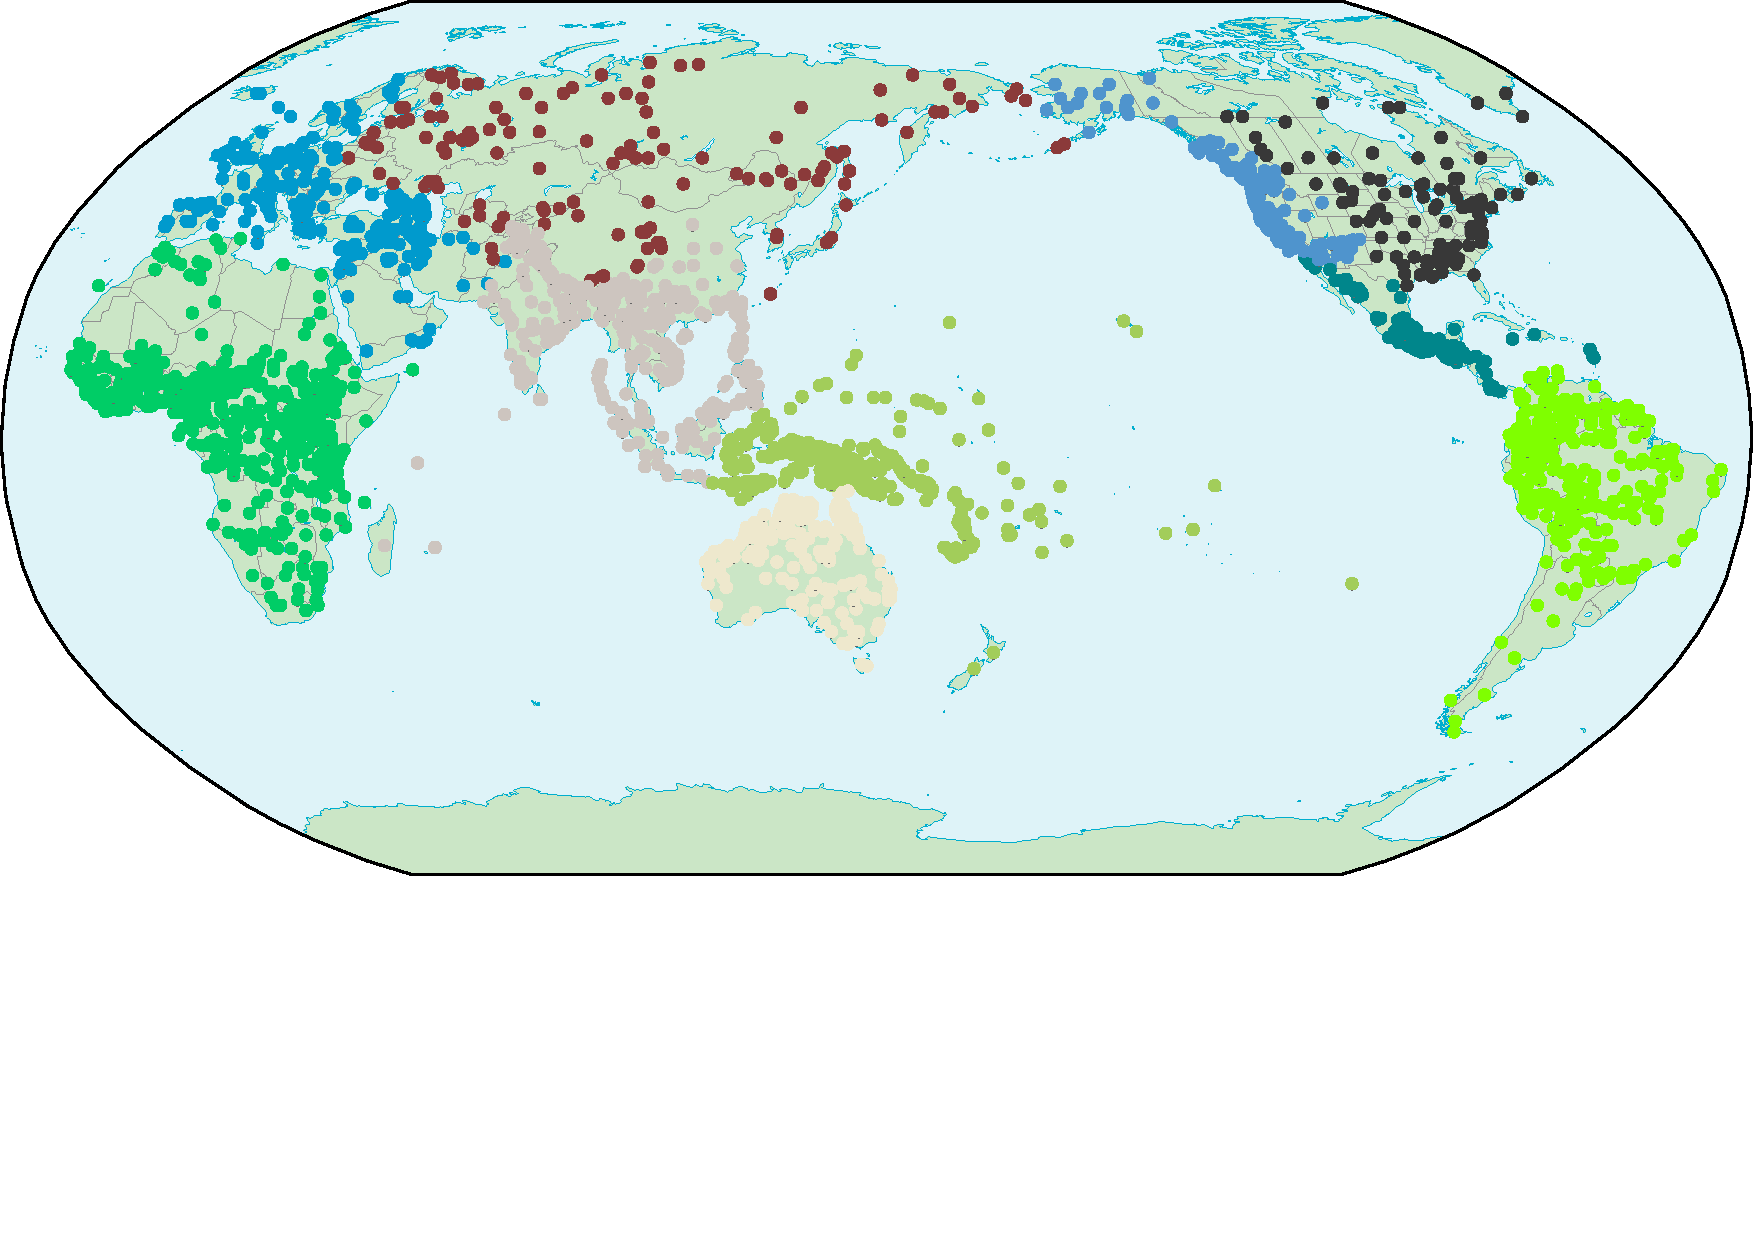
\includegraphics[width=\textwidth]{figures/13/Fig1_Map10continents_s}
\caption{The ten continents of the Autotyp on a world map \citep{Bickel2017}}
\label{fig:Sinne:1}
\end{figure}

For mixed models p-values can be derived by using maximum likelihood ratio tests. This was done by comparing the likelihood ratio of a model with the variable of interest to that of a simpler model without the variable of interest (e.g., \citealt{Baayen2008}; \citealt{Barr2013}).


\subsection{Sampling and data}
\label{sec:Sinne:3.3}


The main data sources were two chapters in the \textit{WALS}, \citet{Corbett2013} on ``Number of genders'' and \citet{Gil2013} on ``Numeral classifiers''. \citet{Corbett2013} has data on 257 languages and \citet{Gil2013} on 400 languages. The cross-section of their data, however, is ``only'' 133 languages (from 106 genera), which is a relatively small proportion of the two samples and not really adequate for modeling the effect of areal and genealogical factors statistically. Moreover, the languages of Eurasia are overrepresented in the cross-section of the samples: the coverage of genealogical diversity (the share of sampled genera from all genera in a macroarea) is 2--3 times greater in Eurasia than in the other five macroareas.

For these reasons, I analyzed more data based on the same principles as in the two main sources in an attempt to increase the sample sizes especially outside Eurasia. I also reanalyzed Corbett's (\citealt*{Corbett2013}) data, since he included pronominal gender in his data, whereas I focus solely on noun gender. By pronominal gender I mean pronouns that reflect gender, such as the English third person pronouns \textit{he} and \textit{she}, which as anaphoric pronouns are often analyzed as part of agreement \citep{Corbett2013}. In the minimal case, pronominal gender can provide the only evidence for a gender system in a language, as was done by \citet{Corbett2013}. In this paper pronominal gender is excluded in order to make gender and numeral classifiers more comparable to one another, because numeral classifiers co-occur with nouns but not usually (or possibly at all) with pronouns. The main data sources for my own data collection were grammar descriptions, scholarly articles (e.g., \citealt{Derbyshire1990}), Nichols' (\citealt*{Nichols1992}) database on gender and numeral classifiers, and general works on linguistic areas and language families (e.g., \citealt{Mithun2001}; \citealt{Janhunen2003}).

The sample contains 360 languages from 252 genera (see Appendix for more information), which is significantly larger compared to what the \textit{WALS} can offer with regard to these variables. I have also attempted to ensure that especially areas that are often less well sampled, such as South America and New Guinea would be sampled to a reasonable degree; in the current paper languages are sampled from roughly 40\% of all the genera in those areas. \tabref{tab:Sinne:2} provides more detailed information about the sample composition by macroarea. Note that the coverage of genealogical diversity of macroareas outside Eurasia is now much better than in the cross-section of the \textit{WALS} chapters: genealogical coverage of Eurasia is not more than 1.2--1.4 times greater than in the other areas.


%
\begin{table}[htb]
\small
\begin{tabular}{@{} l l l l l l l l @{}}
\lsptoprule
&  Afr. & Eur. & Papunes. & Austr. & N.~Am. & S.~Am. & {Total}\footnotemark{}\\
\midrule
Languages & 52 & 69 & 99 & 23 & 58 & 59 & 360 \\
\specialcell{Genera\\ (sample/total)} & 34/81 & 49/87 & 61/139 & 18/44 & 49/102 & 43/108 & 252/544 \\
\specialcell{Genealogical\\ coverage} & 42\% & 56\% & 44\% & 41\% & 48\% & 40\% & 46\% \\
\lspbottomrule
\end{tabular}
\caption{%
Number of sampled languages, number of genera, and the genealogical coverage (share of genera sampled) in each macroarea
}%
\label{tab:Sinne:2}
\end{table}
%
\footnotetext{In Table \ref{tab:Sinne:2} the total number of genera in the \textit{WALS} are not sums of the macroarea-wise counts, because languages from one genus can be spoken in multiple macroareas and thus be counted multiple times. The total is the total of all genera without macroareal partition.}


\section{Results}
\label{sec:Sinne:4}

\subsection{Preliminary results}
\label{sec:Sinne:4.1}

The data come from 360 languages (see Appendix 2). Based on the raw numbers there were 122 languages (34\%) that had only gender, 81 languages (23\%) that had only numeral classifiers, 22 languages (6\%) with both gender and numeral classifiers and 135 languages (38\%) with neither.%
\footnote{Note that the frequency of languages that had both gender and numeral classifiers (6.9\%; counting genera) is similar to the frequency of languages with dominant object-subject word order (6.0\%; counting genera; \citealt{Dryer2013}) which is usually considered to be typologically very rare.} %
All in all, 144 languages had gender (40\%) and 103 languages (29\%) had numeral classifiers. The geographical distribution of the sample languages on the world map is shown in \figref{fig:Sinne:2}. The three smaller maps in \figref{fig:Sinne:2} zoom into three areas where gender and/or numeral classifiers are particularly frequent: 1.~Central Africa, 2.~Southeast Asia, New Guinea, and North Australia, and 3.~South America (see also the discussion below on the areal distribution of gender and numeral classifiers). When counting distinct values in genera gender occurred in 38\% of genera and numeral classifiers in 28\% of genera. These shares suggest that gender is globally more common than numeral classifiers. In the \textit{WALS}-data, the shares for genera that had gender or numeral classifiers were 40\% and 29\%, respectively (\citealt{Corbett2013}; \citealt{Gil2013}). The differences to my data (38\% and 28\%, respectively) are very small, and the 2\% difference in terms of gender can be explained to some extent by the fact that I sampled only noun gender, whereas \citet{Corbett2013} included pronominal gender in his research.

\begin{figure}
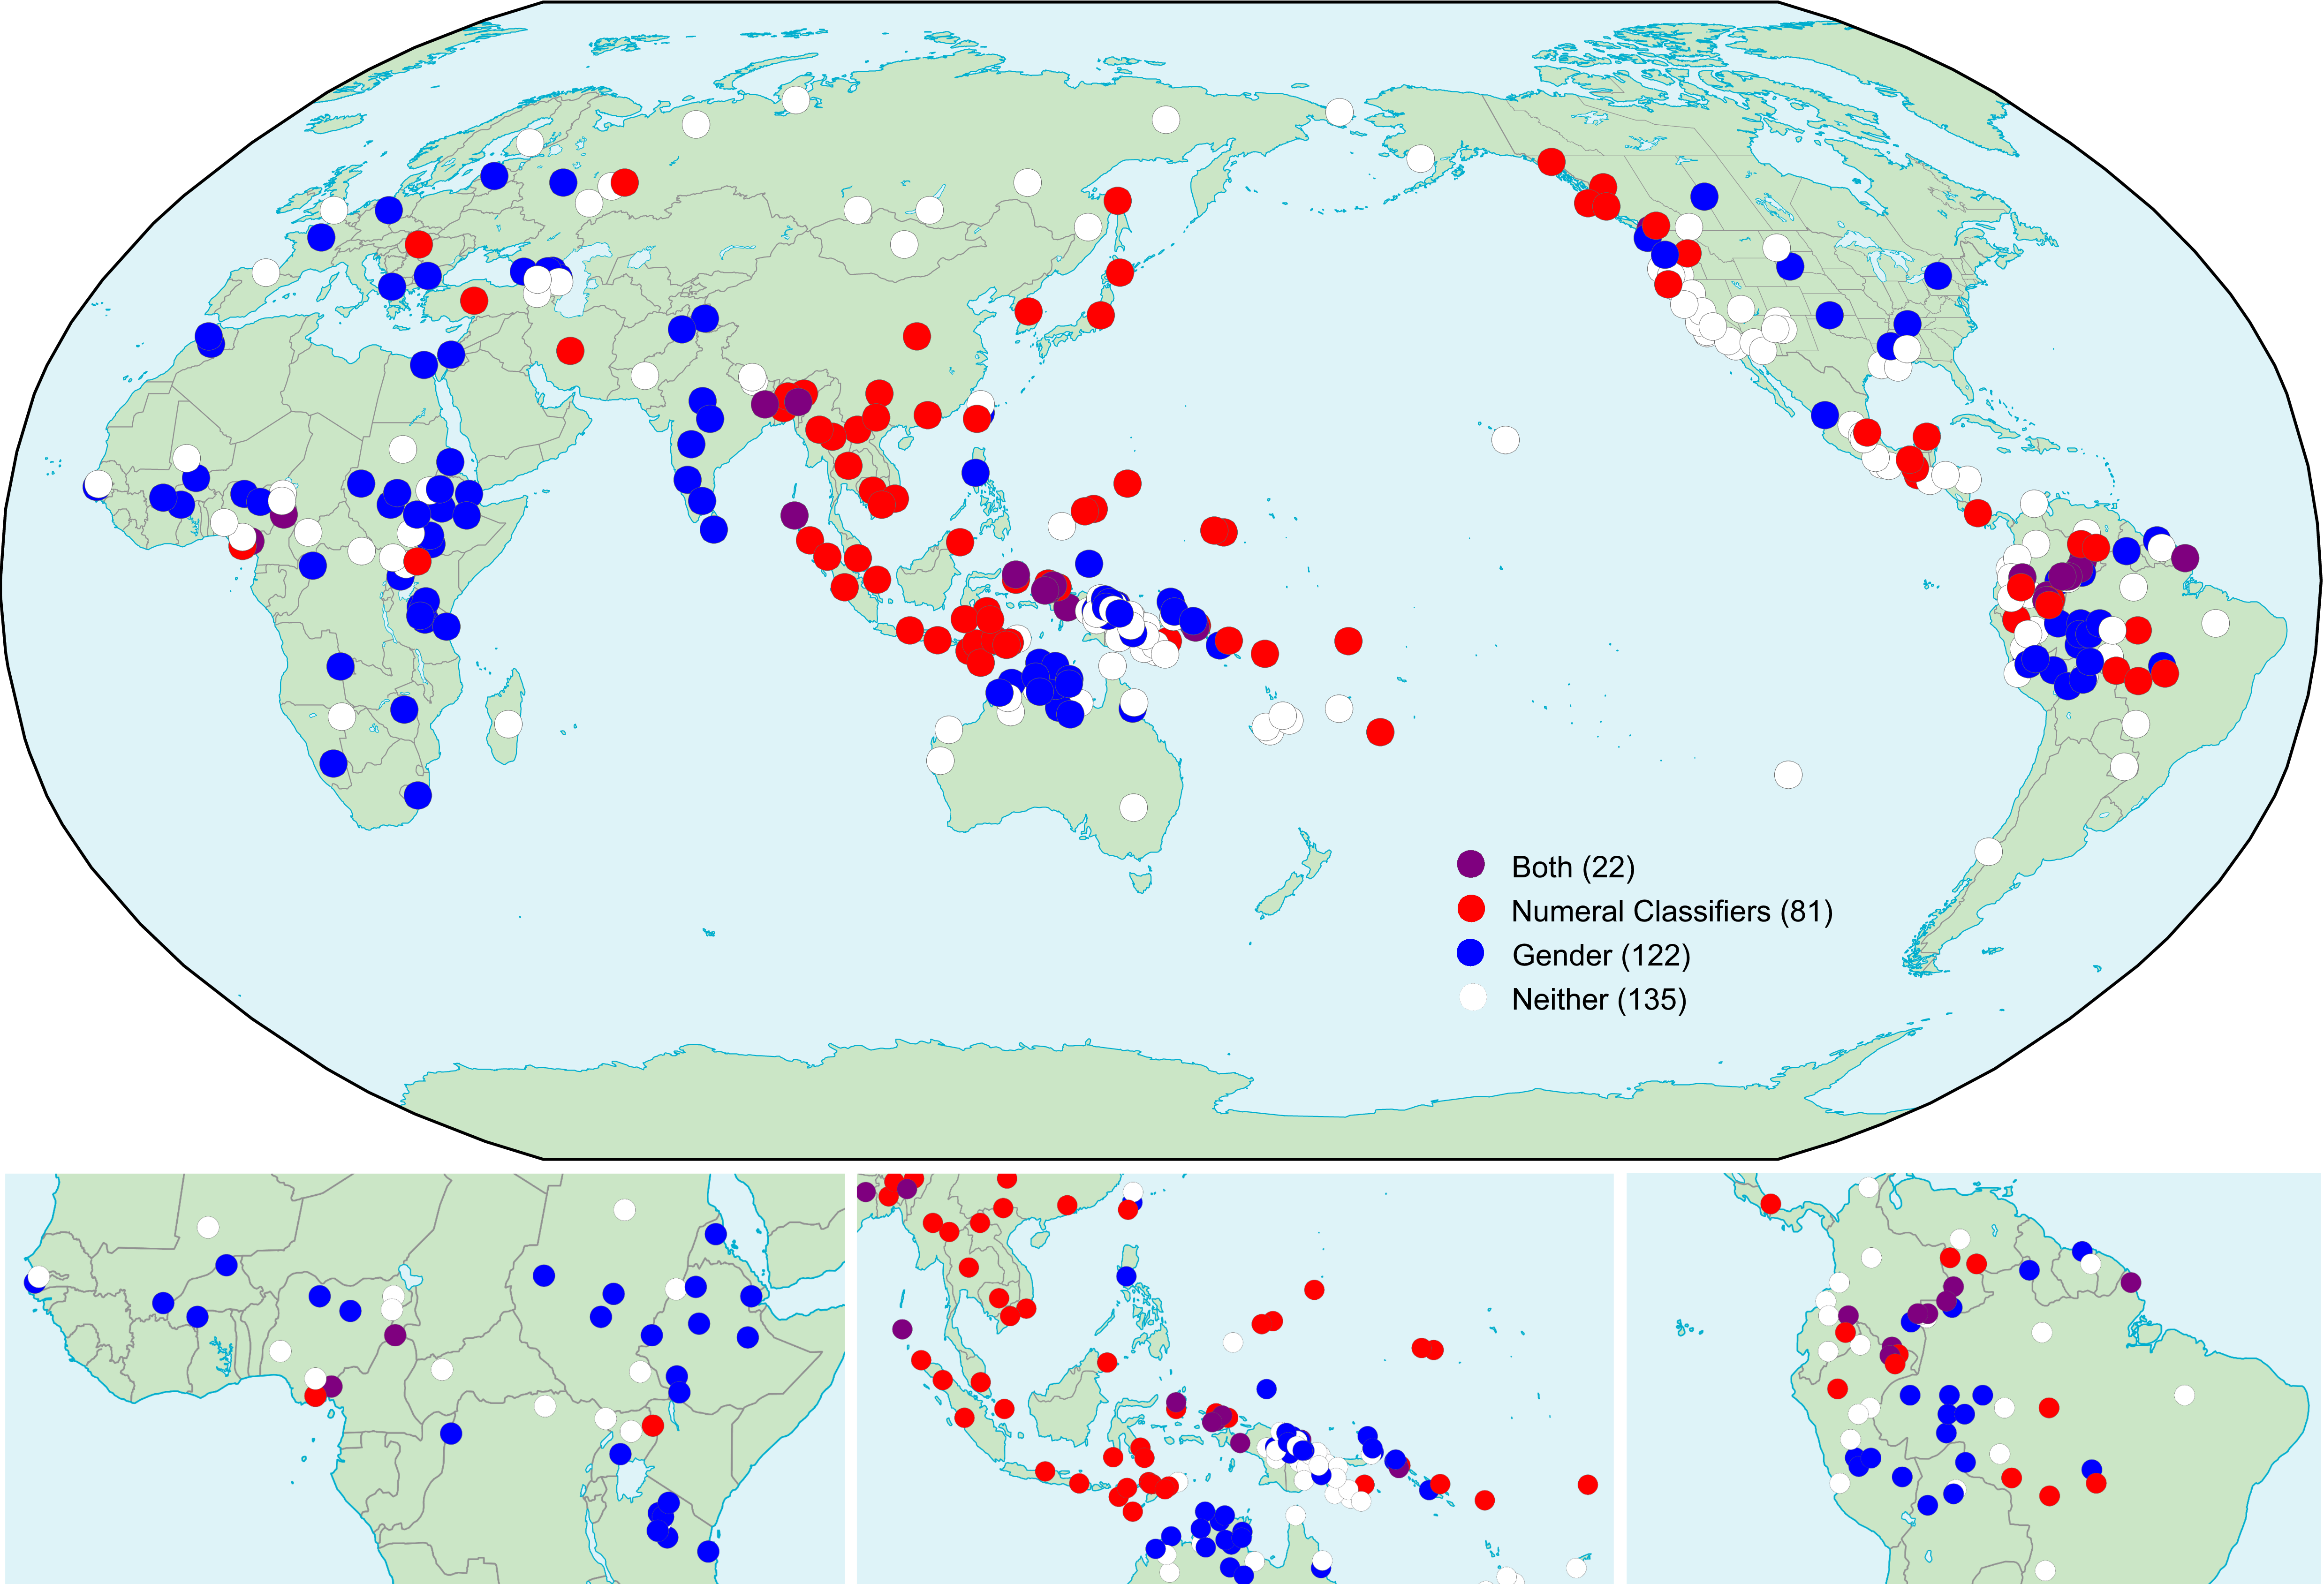
\includegraphics[width=\textwidth]{figures/13/Fig2_MapSample}
\caption{Sample languages on a world map. The three smaller maps at the bottom zoom into central Africa on the left, Southeast Asia and New Guinea in the middle, and the Northern half of South America on the right.}
\label{fig:Sinne:2}
\end{figure}

\citet[1]{Aikhenvald2000} estimates that ``[a]lmost all languages have some grammatical means for the linguistic categorization of nouns and nominals.'' While here my focus is not on all types of noun classification, it is worth noting that 63\% of the sample languages (n~=~225) had either gender or numeral classifiers or both and this may suggest an overall preference for languages to develop some type of noun classification (but since 38\% of my sample languages had neither gender nor numeral classifiers, the estimation that almost all languages have some type of noun classification is too strong). If we count how many genera had languages with either type of noun classification, roughly 58\% of genera (n = 152) had either gender or numeral classifiers or both, while 42\% of genera (n = 111) had neither gender nor numeral classifiers. According to exact binomial test, this distribution is statistically significant (one-tailed p = 0.0067). This result provides evidence that languages prefer to develop either gender or numeral classifiers or both rather than not to develop any type of noun classification. Since my counts do not include possessive classifiers and noun classifiers, it is plausible that if those other types of classifiers had been included, the preference would have been even stronger.

A heatmap of the distribution of gender and numeral classifiers is shown in \figref{fig:Sinne:3} (counts in genera). If we count distinct values in genera, and perform Fisher's Exact test to the data, then there is a statistically significant inverse dependence between gender and numeral classifiers (p = 0.005). According to this distribution, gender is 2.3 times less likely in genera that have languages with numeral classifiers than in those that lack numeral classifiers. However, counting genera is a crude way of controlling for genealogical inheritance (cf.\ \sectref{sec:Sinne:3.2}) and this test also does not take into account possible areal diffusion. Those issues will be more properly dealt with in the next section using generalized mixed logistic regression.

\begin{figure}
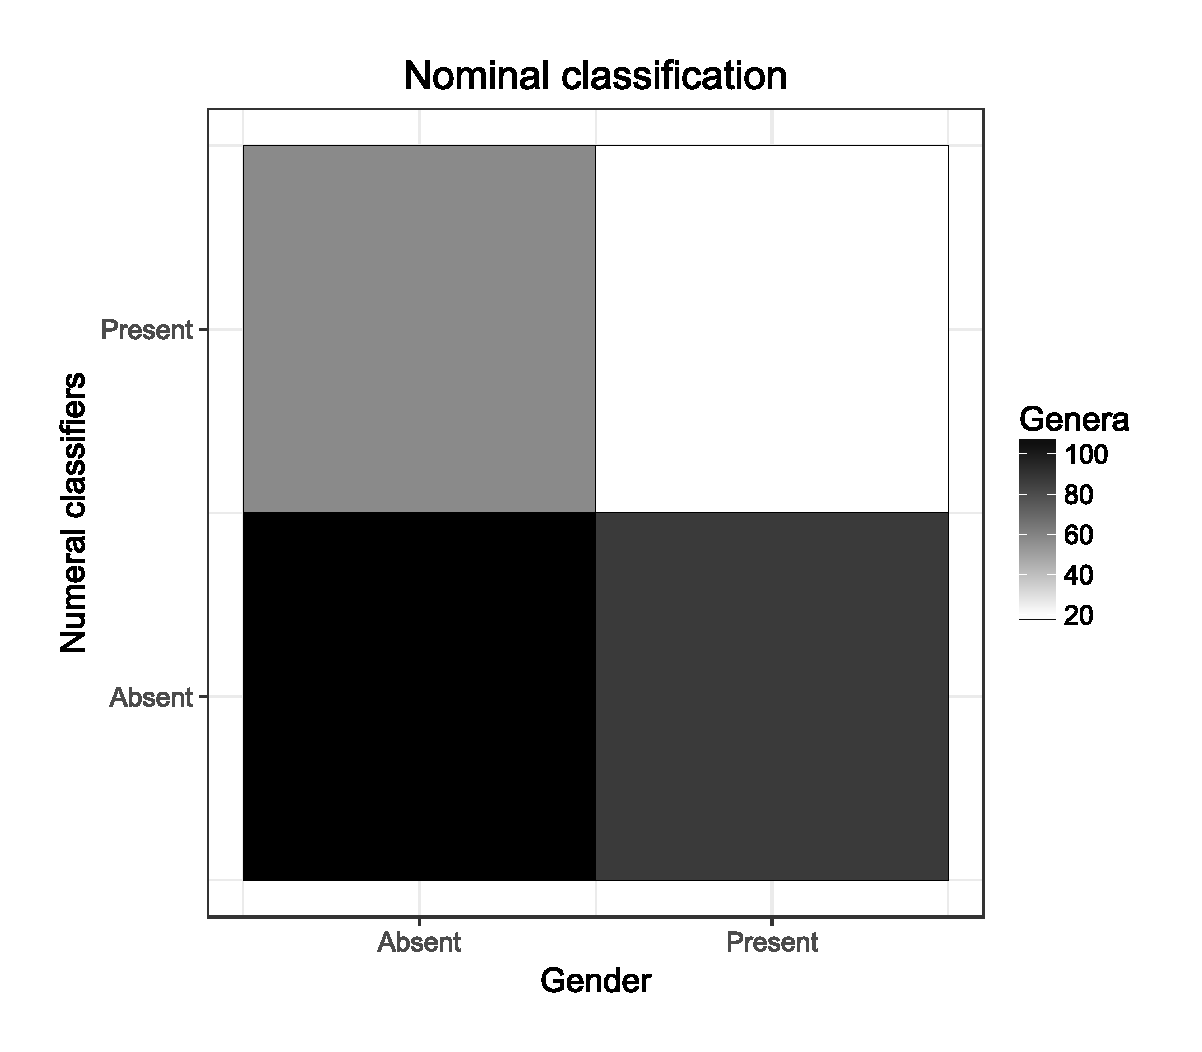
\includegraphics[width=.6\textwidth]{figures/13/Fig3_heatmap}
\caption{%
Heatmap of the distribution of gender and numeral classifiers (counts in genera).
}%
\label{fig:Sinne:3}
\end{figure}

The data also allows to estimate genus-internal diversity and stability of gender and numeral classifiers. There were altogether 56 genera with more than one sampled language and in 12 of these (21\%) there was diversity in terms of gender (that is, some languages with gender and some without gender). This means that 79\% of genera were uniform in either having gender or not having gender and this distribution is statistically significant (exact binomial test; two-tailed; p = 0.00002). As for numeral classifiers, there was diversity in 11 genera (20\%). This means that 80\% of genera were uniform in either having numeral classifiers or not having them and this distribution is statistically significant (exact binomial test; two-tailed; p = 0.000005). If we take these figures as a proxy for the stability of gender and numeral classifiers within genera, both features seem to be relatively stable (see \citealt[433--434]{Bickel2013b} for similar conclusions for pronominal gender; also \citealt[196--202]{Dahl2004}).

A few words can also be said concerning the areal distributions of gender and numeral classifiers. As for numeral classifiers, it has been noted by Johanna Nichols and colleagues that numeral classifiers cluster in languages spoken around the Pacific Ocean (e.g., \citealt[132--133]{Nichols1992}; \citealt[366--367]{Nichols1996}; \citealt[299]{Nichols2003}). On the basis of the distributions in \figref{fig:Sinne:2}, this claim seems largely true, although some languages in Africa, Europe and Central Asia also have numeral classifiers, while no language in Australia has them \citep[121--124]{Aikhenvald2000}.%
\footnote{The observation that there are no numeral classifiers in Australian languages may be related to their numeral systems in general. The existence of numeral classifiers presupposes that a language has a numeral system \citep[99]{Aikhenvald2000}. However, many Australian languages have numbers only for the low numerals (e.g., from one to three), but these do not necessarily form a separate part of speech (see \citealt[100]{Aikhenvald2000} and references there). The reason why there are no numeral classifiers in Australia may thus be related to the fact that in many languages in this area numerals either do not exist at all as a separate part of speech or numbers are expressed through other larger parts of speech. However, other types of classifiers, such as noun classifiers, are common in Australian languages (\citealt[82]{Aikhenvald2000}; see also \citealt{Plaster2007}).} %
Here I use GLMM to evaluate Nichols' claim whereby numeral classifiers are more likely to occur in languages spoken in the Circum-Pacific. Following \citet{Bickel2006} I define Circum-Pacific as encompassing the Americas, Oceania (including New Guinea and Australia), Southeast Asia, and the Northeastern Coast of Asia. Following \citet{Nichols2003}, I include mainland and island Southeast Asia in this area. I then compare the distribution of numeral classifiers in this large area against the rest of the world (that is, Africa and Eurasia except for Southeast Asia and Northeastern Coast of Asia). \figref{fig:Sinne:4} presents the sample languages inside and outside the Circum-Pacific area on a world map. An association plot of the distribution of numeral classifiers inside and outside the Circum-Pacific area is shown in the left panel of \figref{fig:Sinne:5}.

I modeled numeral classifiers as the dependent, area as a binomial predictor (whether a language is spoken inside or outside the Circum-Pacific area), and the \textit{WALS} families as a random intercept. According to the mixed logistic regression, languages spoken in the Circum-Pacific area were significantly more likely to have gender than languages spoken outside this area (logit estimates: 2.3 $\pm$ 1.2 (standard errors); $\chi^2$ (1) = 5.1; p = 0.024). As an alternative approach I used stocks (the highest level of genealogical classification in the \textit{Autotyp}) as a random intercept. According to this model design, languages spoken in the Circum-Pacific area were again significantly more likely to have numeral classifiers than languages spoken outside this area (logit estimates: 2.6 $\pm$ 1.3 (standard errors); $\chi^2$ (1) = 6.0; p = 0.014). When interpreting the coefficients as odds ratios in this model, languages spoken in the Circum-Pacific region were thirteen times more likely to have numeral classifiers than languages spoken outside this region.

\begin{figure}
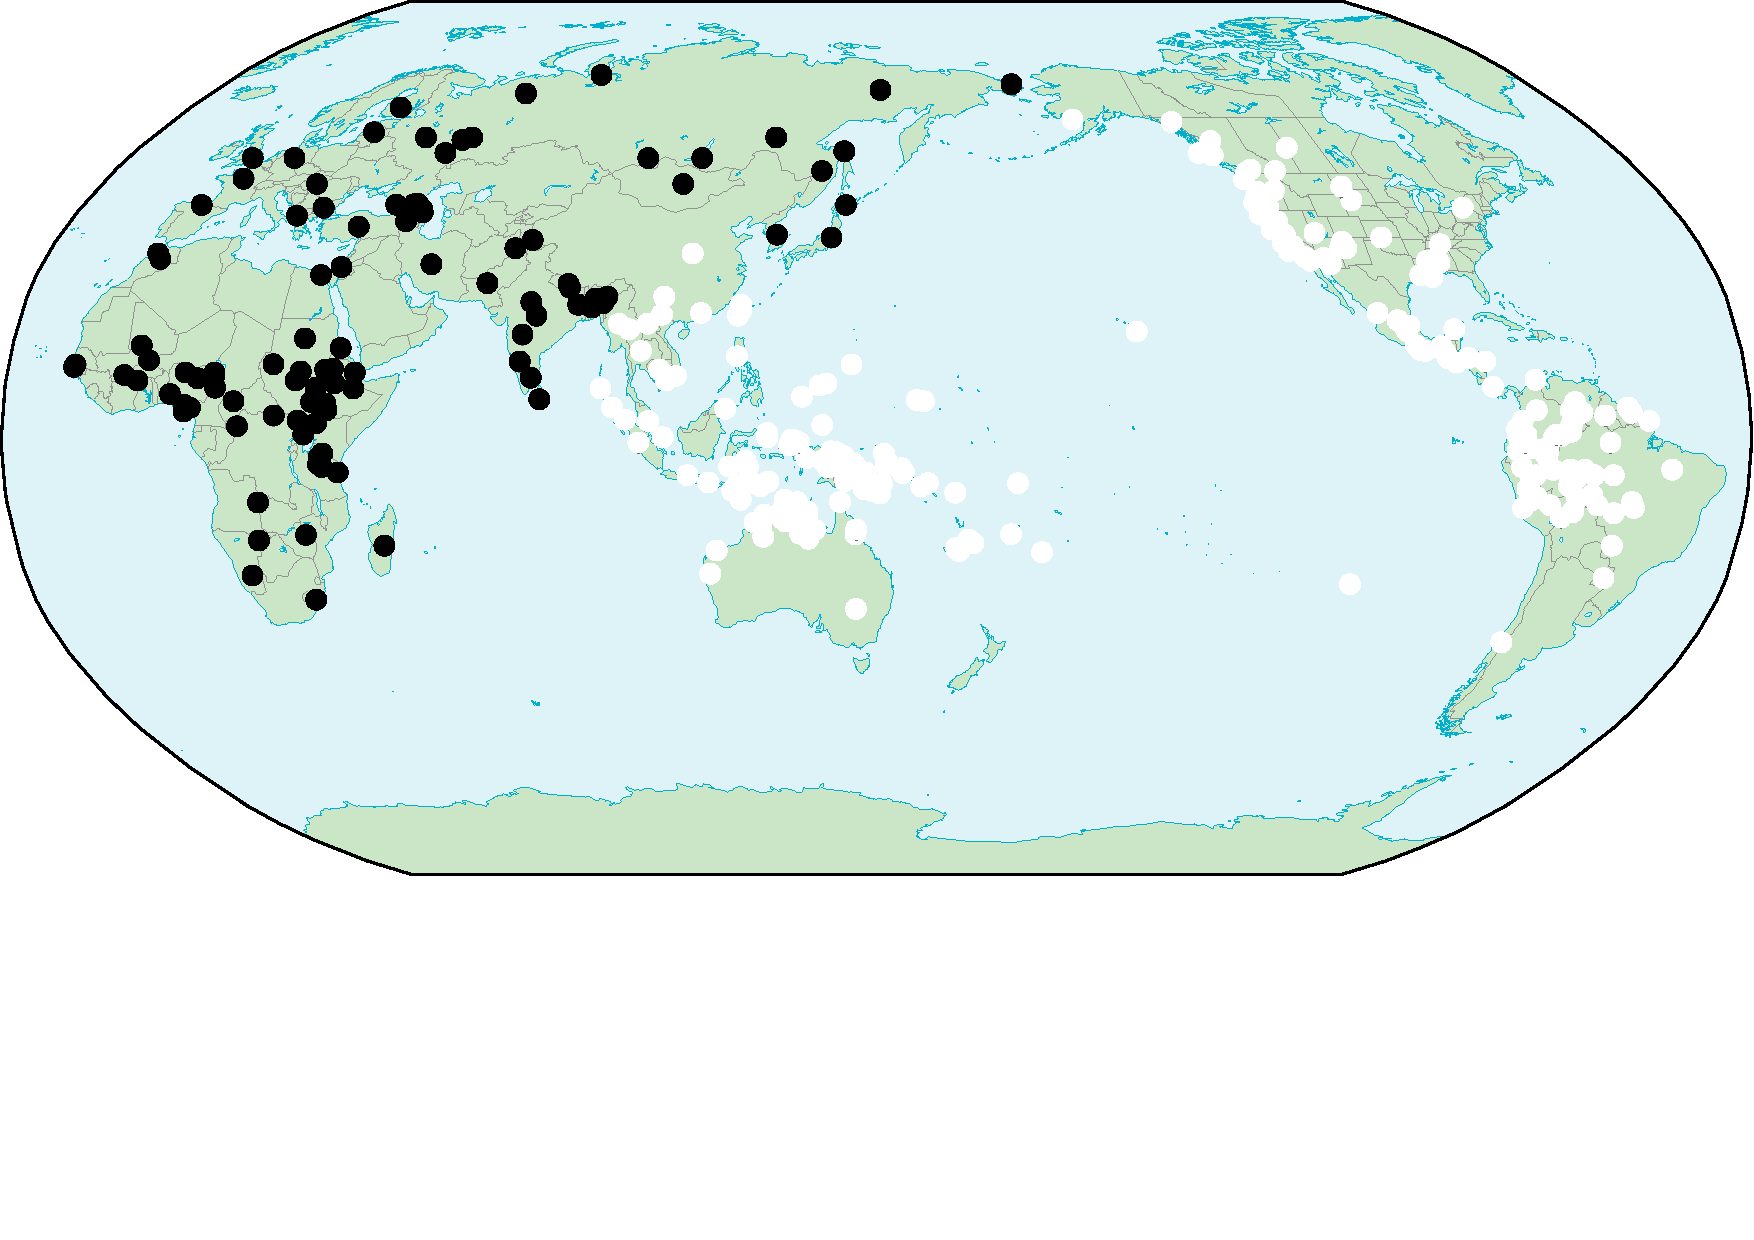
\includegraphics[width=\textwidth]{figures/13/Fig4_MapCircumPacific_s}
\caption{Sample languages on a world map according to area (white = Circum-Pacific area, black = the rest)}
\label{fig:Sinne:4}
\end{figure}

The areal distribution of gender has not been in focus very often, but what has been said about it in the literature (simplifying a little) is that gender is not too frequent in the Americas and in the Austronesian languages, whereas it tends to cluster especially in Africa, Europe, Caucasus and the Indian Peninsula as well as in Australia (\citealt[1--2]{Corbett1991}; \citealt[130--132]{Nichols1992}; \citealt{Corbett2013}).%
\footnote{\citet[130--132]{Nichols1992} proposes that most gender-languages occur in hotbeds, that is, areas in which gender occurs in most languages of the area, but they come from diverse families and occur in diverse forms. Because my focus is not on the formal aspects of gender marking, her proposal cannot be statistically tested in this paper.} %
This distribution sounds like the opposite to that of numeral classifiers. I therefore compared the distribution of gender in the Circum-Pacific area against the rest of the world as above in the case of numeral classifiers, first modeling \textit{WALS}{}-family as random intercept. An association plot of this distribution is shown in the right panel of \figref{fig:Sinne:5}.

\begin{figure}
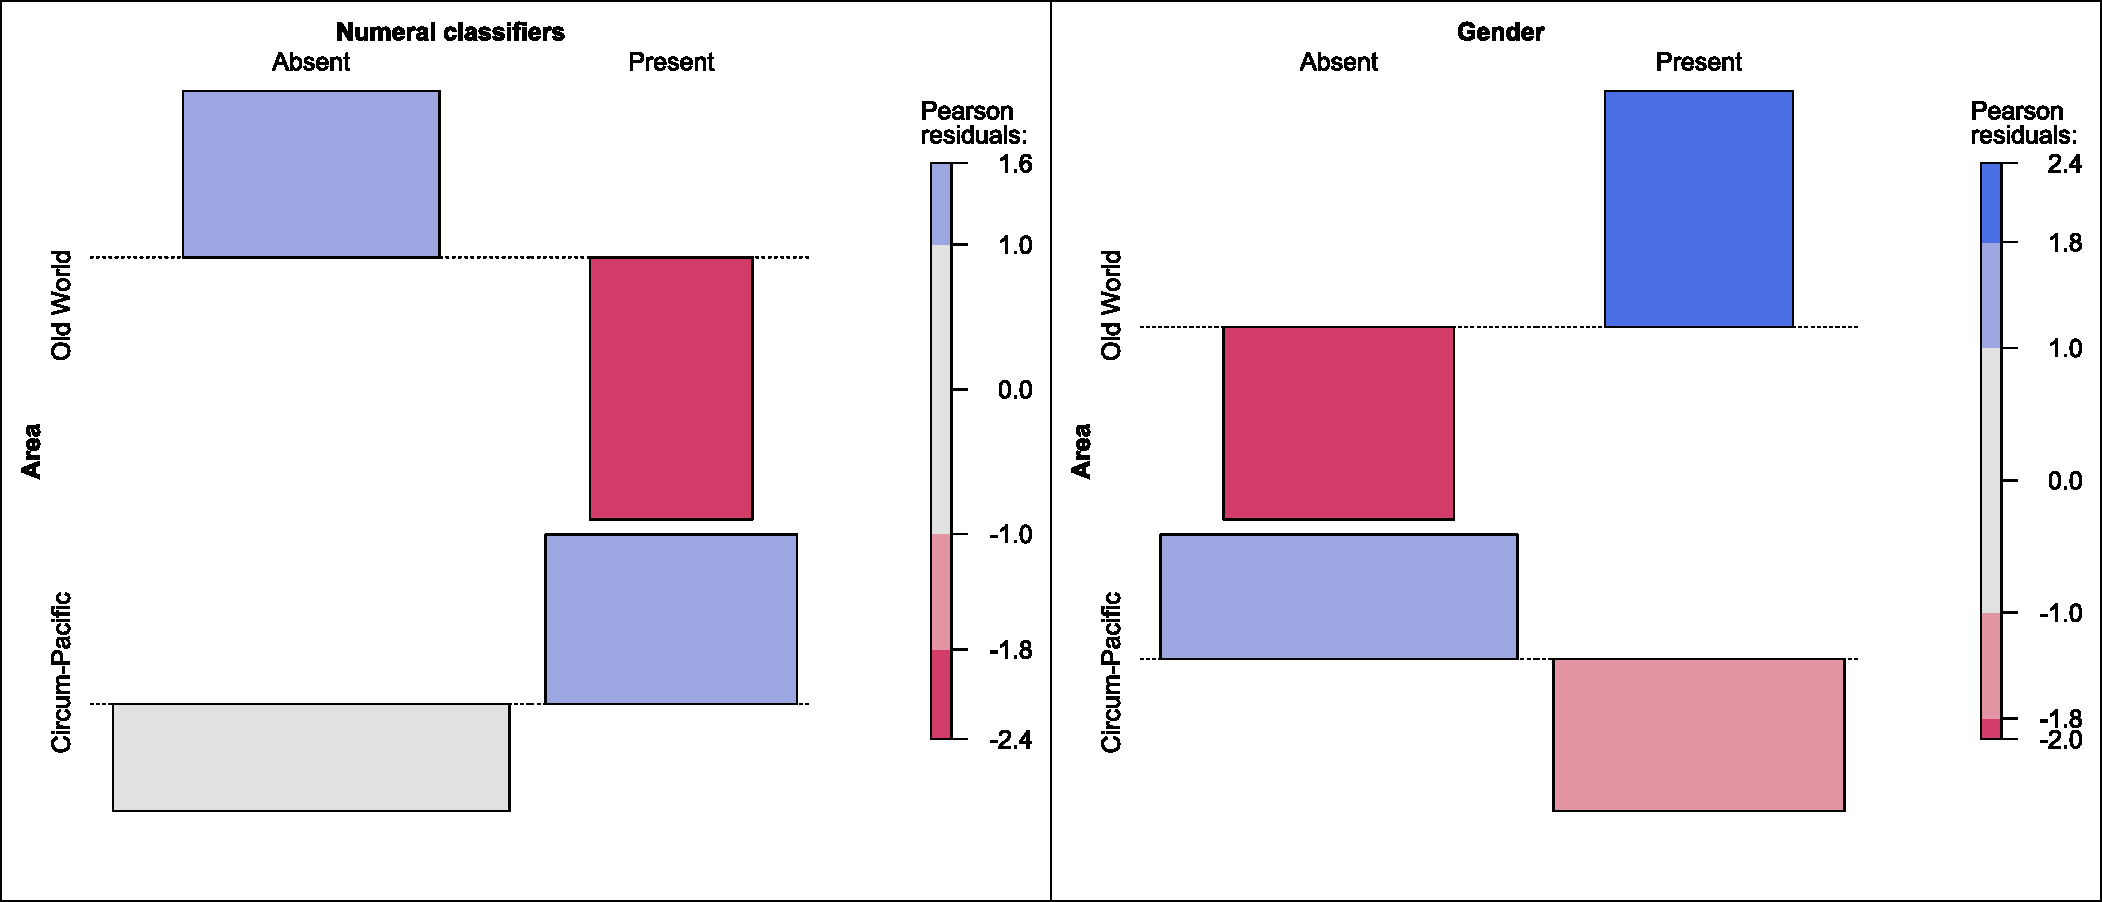
\includegraphics[width=\textwidth]{figures/13/Fig5_assocplot}
\caption{Association plots of the distribution of numeral classifiers (left panel) and gender (right panel) inside and outside the Circum-Pacific. Positive Pearson residuals (blue color) indicate that the cell values were greater than expected and negative Pearson residuals (red) indicate that the cell values were smaller than expected.}
\label{fig:Sinne:5}
\end{figure}

According to the mixed logistic regression, languages spoken in the Circum-Pacific area were less likely to have gender than languages spoken outside this area (logit estimates: $-0.7 \pm 0.5$ (standard errors)), but this relationship was not statistically significant ($\chi^2$ (1) = 1.8; p = 0.18). As an alternative approach I used stocks (the highest level of genealogical classification in the \textit{Autotyp}) as a random intercept. According to this model design, languages spoken in the Circum-Pacific area were significantly more likely to have numeral classifiers than languages spoken outside this area (logit estimates: $-1.1 \pm 0.5$ (standard errors); $\chi^2$ (1) = 4.2; p = 0.041). When interpreting the coefficients as odds ratios in this model, languages spoken in the Circum-Pacific were about three times less likely to have gender than languages spoken outside this region.

The conclusion from these distributions is that there is an inverse relationship between gender and numeral classifiers in the languages of the world. On the other hand, there is a roughly complementary areal distribution of gender and numeral classifiers so that numeral classifiers are more likely to occur in the Circum-Pacific region than outside it, whereas gender has the opposite distribution. One consequence of these results could be that the inverse relationship between gender and numeral classifiers is simply an outcome of their biased areal distributions. However, as will be shown in the following section, gender has this inverse relationship to numeral classifiers independently of geographical areas.


\subsection{Testing the main hypothesis}
\label{sec:Sinne:4.2}

The hypothesis that an inverse relationship exists between gender and numeral classifiers was tested with generalized mixed effects models. I constructed a model using the \textit{WALS} families as a grouping factor for genealogical affiliation and the ten continents from the \textit{Autotyp} as the grouping factor for areas. This is my main model and it is also a maximal model that has all the theoretically motivated random intercepts and slopes included. In recent research, it has been suggested that maximal models are preferred in mixed models and especially that models without random slopes may produce spurious results (\citealt{Schielzeth2009}; \citealt{Barr2013}).

According to the mixed logistic regression, languages with numeral classifiers were significantly less likely to have gender than those with no numeral classifiers (logit estimates: $-2.1 \pm 1.1$ (standard errors); $\chi^2$ (1) = 7.7; p = 0.0056). The negative coefficient and the highly significant p-value suggest that the hypothesis is confirmed. A closer inspection of the random effects in \tabref{tab:Sinne:3} confirms that the random structure is feasible: the correlation terms between the random intercept and the random slopes for both family and continent are not too large ($0.41$ and $-0.09$, respectively).

\begin{table}[htb]
\begin{tabularx}{\textwidth}{XXXXX}
\lsptoprule
\multicolumn{2}{l}{Random effects:} &  & \\
 Groups &  Name &  Variance &  Std.Dev. &  Corr\\
\midrule
family & (Intercept) & 2.35 & 1.53\\
& clfyes & 1.48 & 1.22 & 0.41\\
continent & (Intercept) & 0.63 & 0.80\\
& clfyes & 0.53 & 0.73 & $-0.09$\\
\lspbottomrule
\end{tabularx}
\caption{Random effects for the maximal model}
\label{tab:Sinne:3}
\end{table}

I further tested the validity of the result with a parametric bootstrap method (\citealt{Halekoh2014}). This method returns the fraction of those simulated likelihood ratio test values that are larger or equal to the observed likelihood ratio test value. Using 2 000 simulations the parametric bootstrap derived p-value was 0.0398. Although this p-value is larger than the one derived from the $\chi^2$-distribution (p = 0.0056), it still confirms that the inverse relationship between gender and numeral classifiers is significant and holds independent of geographical area and language families. When interpreting the coefficients as odds ratios, we can conclude that gender is about eight times less likely to occur in a language when that language already has a numeral classifier compared to languages without numeral classifiers. To put it in another way, there is a statistical implicational universal in languages that if a language has numeral classifiers, then it is likely not to have gender but if a language does not have numeral classifiers then it is likely to have gender. The results were then tested by using an alternative genealogical classification and three alternative areal configurations. These tests and their results are presented in Appendix 1. In all these additional models the result was the same as here: an inverse and significant relationship occurred between gender and numeral classifiers.

I then fitted a competing model choosing numeral classifiers as the dependent and gender as the predictor. I modeled the random structure as in the model above. \textit{WALS}{}-families were used to model genealogical affiliation and the ten \textit{Autotyp} continents were used to model geographical areas. According to the mixed logistic regression, languages with gender were \emph{more} likely to have numeral classifiers than languages with no gender (logit estimates: $1.0 \pm 2.2$ (standard errors), but this relationship was not statistically significant ($\chi^2$ (1) = 0.21; p = 0.64). But the random structure of this competing model suggests that the model may be too complex to fit to the data. The correlation between the random intercepts and slopes for both family and continent are $-1.0$ and the variances for family are extremely large (93 for the random intercept and 21 for the random slope). These problems with the random structure may explain why the relationship between numeral classifiers and gender was positive and not negative as expected (cf.\ Appendix 1). To further double-check this I refitted the competing model but using the six macroareas of the \textit{WALS} as the geographical area-factor (see Appendix 1 for the distribution of these macroareas on a map). According to this model, languages with gender were \textit{less} likely to have numeral classifiers than languages with no gender (logit estimates: $-1.8 \pm 2.5$ (standard errors), but this inverse relationship was not statistically significant ($\chi^2$ (1) = 0.0; p = 1.0). I then refitted the competing model using the 24 areas of the \textit{Autotyp} as the geographical area-factor (see Appendix 1 for the distribution of the 24 areas on a map). According to this model, languages with gender were again less likely to have numeral classifiers than languages with no gender (logit estimates: $-4.0 \pm 3.4$ (standard errors) and this inverse relationship was statistically significant ($\chi^2$ (1) = 4.8; p = 0.028).

All in all the results of the competing models were very variable and depended on the areal configuration used, whereas the results of the main model (and the additional models in Appendix 1) were consistent regardless of how genealogical affiliation and geographical areas were coded. I interpret these results to mean that numeral classifiers are more likely to have an effect on gender rather than the other way round, which is exactly what has been suggested in the literature (\sectref{sec:Sinne:3.2}).

The results of the mixed effects logistic models suggest that there is a statistically significant complexity trade-off between gender and numeral classifiers. This result was also independent of how geographical area and language family were coded. However, because the data contained many counterexamples against the trade-off the generalization is not an absolute universal. Many languages, for instance, had neither gender nor numeral classifiers, and therefore the generalization must be understood as a probabilistic universal.%
\footnote{For instance, all or almost all languages in Quechuan, Oto-Manguean, Uto-Aztecan, and Trans-New Guinea language families had neither gender nor numeral classifiers, whereas some languages in the Arawakan, Tucanoan, and West Papuan families had both gender and numeral classifiers (e.g.\ Palikur in (\ref{ex:Sinne:1})).}


\section{Discussion}
\label{sec:Sinne:5}

The distribution of gender and numeral classifiers and the complexity trade-off between them raise questions that require explanations. Three issues in particular require attention. Why is there a trade-off between gender and numeral classifiers? Why are their areal distributions so biased? Why are languages more likely to have some noun classification system rather than no noun classification at all? Within the limits of this paper I confine myself to providing some preliminary thoughts on possible explanations.

The central question here is why there is a complexity trade-off between gender and numeral classifiers? Two relevant issues are discussed here. First, from a functional point of view gender and numeral classifiers tread the same functional domain, that is, they encode semantically-pragmatically closely related functions across languages \citep[293]{Miestamo2007}. These functions have to do primarily with individuation and reference-identification (or `reference-tracking'), although other functions are also shared across gender and numeral classifier systems (\citealt[293--294]{Contini-Morava2013}). Because gender and numeral classifier systems share these similar functions, the inverse correlation between these variables can be explained functionally by economy and distinctness. The rationale for this explanation is the following. Economy and distinctness are functional motivations that relate to the amount of linguistic structure, economy for keeping it minimal, and distinctness for preserving distinctions in linguistic structure. Now, if a language has already developed a system of noun classification (e.g., gender), it is inefficient and redundant for that language to develop another type of nominal classification (e.g., numeral classifiers) to serve a similar set of functions (e.g., \citealt{Hawkins2004}; \citealt{Sinnemaeki2014}). The small likelihood of developing multiple systems of noun classification is, therefore, a matter of the Zipfian principle of least effort or economy and its interaction with distinctness: linguistic structures are kept minimal without losing distinctness.

The second issue is diachronic in nature. If a language loses its noun classification system, it may redevelop another type via reanalysis. For instance, gender markers have been lost in many Iranian and Indic languages, but many of these languages have developed numeral classifiers. In Bengali this resulted in reinterpreting the old feminine forms in terms of numeral classifiers. In Africa, Ogonoid (also called Kegboid) languages, such as Kana (Ogonoid; Niger-Congo), lost their noun class system and instead developed numeral classifiers, which are very rare in Africa. Overall, noun classification may thus be a rather stable feature in language although the particular classification system may be lost. (See \citealt[379--381]{Aikhenvald2000} and references.)

While multiple systems of noun classification are possible, they are rare (see \sectref{sec:Sinne:4.1}). One reason for languages to develop more than one system of noun classification is language contact. For instance, Santali (Munda; Austro-Asiatic) has two gender systems as well as numeral classifiers. One gender system is native to Santali and it distinguishes animate from inanimate, while the other system is borrowed from Indo-Aryan and it distinguishes male from non-male \citep[39]{Ghosh2008}. In (11), the noun \textit{Kali-idol} triggers object gender agreement on the verb, which is marked by the third person object clitic -\textit{e} that is reserved for animate beings, but it also requires the use of the a numeral classifier -\textit{taŋ}.

\ea
\label{ex:Sinne:11}
\langinfo{Santali}{Austro-Asiatic}{\citealt[39]{Ghosh2008}}\\
\gll uni mit'-taŋ kəli-boŋga benao-akad-e-a-e \\
\textsc{3sg.m} one-\textsc{clf} Kali-idol make-\textsc{prf.a-3sg.obj-fin-3sg.sbj}\\
\glt ``He has made a Kali idol.''\\
\z

Numeral classifier systems can also be borrowed, as seems to have happened in Malto (Dravidian). Malto presumably borrowed numeral classifiers from Magahi (Indic; Indo-European) and elaborated the system subsequently \citep[117--118]{Emeneau1980}. Besides the numeral classifier system Magahi also has a gender system \citep{Steever1998}. These are illustrated in (\ref{ex:Sinne:12}).

\protectedex{%
\ea
\label{ex:Sinne:12}
\langinfo{Malto}{Dravidian}{\citealt[363, 372]{Steever1998}}\\
\begin{xlist}
\ex
\gll t\=ini jen maler \\
three \textsc{clf} man.\textsc{pl} \\
\glt ``Three men.''\\
\ex
\gll r\=ajah awḍah.\\
king.\textsc{m.nom} say.\textsc{pst.3sg.m}\\
\glt ``The king said.''
\end{xlist}
\z
}%

Language contact is also one reason for why multiple systems of noun classification get reduced. For instance, Retuara (Tucanoan) has lost its classifier system and retained only a gender system because of language contact with Yucuna (Arawakan; see \citealt[386]{Aikhenvald2000} and references).

The kinds of ``compensating'' mechanisms discussed above, motivated by economy and distinctness and manifest in diachronic change, may be found in other areas of grammar as well (e.g., \citealt{Sinnemaeki2014}). Ultimately economy and distinctness are grounded in language processing and are like the two sides of the same coin. As a processing principle economy is a matter of `minimize all you can', which means that all unnecessary distinctions can be dispensed so that distinctness is not lost (\citealt{Bornkessel-Schlesewsky2009}). In terms of language change, complexity trade-offs may be seen as adaptive processes where linguistic structure adapts to preferences in language processing (\citealt{Sinnemaeki2014b}; \citealt{Bickel2015}). In noun classification this adaptation shows up in the fact that while the majority of the world's languages have a system of noun classification (\sectref{sec:Sinne:4.1}), there is a tendency in languages not to develop more than one such system.

This leads us to another important question raised by the results, namely, why the presence of noun classification is preferred over its absence across languages (\sectref{sec:Sinne:4.1}). One relevant issue in this regard is the discussion on language complexity that has taken place during the past 15 years. Many researchers have argued that gender is relatively devoid of meaning (not marking real-world categories), adds unnecessary complexity to language, and therefore tends to be lost in situations that involve heavy language contact by adult learners (e.g., \citealt[129]{McWhorter2001}; \citealt[25]{Kusters2003}; \citealt[155--166]{Trudgill2011}). It has also been claimed that classifier systems are at a corresponding level of complexity compared to gender systems (\citealt[136--141, 147--148]{Riddle2008}). Although numeral classifiers tend to mark real-world categories \textendash{} and in this sense are more semantically based \textendash{} they have been analyzed in the same way as gender, adding unnecessary complexity to language (e.g., \citealt[22]{McWhorter2007}). Some quantitative evidence for the loss of gender complexity comes from pidgins, which tend to lose especially agreement categories, such as gender (\citealt{Roberts2008}). Against this background it is surprising that there seems to be a preference for languages to develop this kind of grammatical marking, be it gender or numeral classifiers, if it really is unnecessary for human communication.

One possibility for this preference may be functional. The shared functions of gender and numeral classifiers deal primarily with individuation and reference-identification, but gender shares further functions with other types of classifiers as well, including the derivational expansion of the lexicon (\citealt{Contini-Morava2013}; see also \citealt[136--141]{Riddle2008}). These functions may be central enough in communication that there is a general preference in languages to develop some type of noun classification to serve these functions. On the contrary, especially gender marking may sometimes lead to tracking failure and ambiguity and there are also grounds to believe that the referential functions of gender (and possibly also those of classifiers) are important only in languages which have many classes in their noun classification system \citep[158--159]{Trudgill2011}. In this sense it is unclear whether the above functions of noun classification are important enough to attract and sustain noun classification in languages.

Another possible explanation is based on the simple fact that noun classification groups nouns into classes. Even languages that do not have noun classification may have some other forms of grouping nouns into subcategories. One such example is declensional type (or inflectional class), which is a way of classifying nouns into groups depending on how they inflect for grammatical categories such as number and case (e.g., \citealt[67--68]{Kramer2015}). \citet[583--584]{Dahl2000} makes the strong point that sometimes inflectional classes actually look like gender distinctions and some of them could be analyzed as gender. Thus, noun classification and inflectional classes share the fact that they group nouns into subcategories. This leads me to the following preliminary conclusion for why there is a preference to develop noun classification in the languages of the world: languages prefer to classify nouns into subcategories and languages reach this goal in different ways by using gender, classifiers, inflectional classes, or some other means.

The third question that the results raised is why the areal distributions of gender and numeral classifiers were so biased. Since the origin and/or distribution of gender and classifiers have been discussed in multiple publications (e.g., \citealt{Corbett1991}, \citealt{Corbett2013}; \citealt{Nichols1992}, \citealt{Nichols2003}; \citealt{Aikhenvald2000}; \citealt{Luraghi2011}; \citealt{Gil2013}; \citealt{Passer2016b}), I will only provide some observations here.

There is increasing evidence suggesting that classifiers spread through language contact more easily than gender does and therefore serve as strong areal markers \citep[730]{Seifart2010}. In addition, what tends to diffuse is often the pattern of classifiers and not the actual markers (in terms of \citealt[234--237]{Matras2009}); it is rather the native words that are employed for the purpose of an incipient classifier system. Gender systems do not spread so easily because agreement systems are less easily borrowed, although parts of the systems may be borrowed \citep[386--388]{Aikhenvald2000}. Since the pattern of numeral classifiers may be relatively easy to spread, whereas the pattern of gender tends not to spread easily, it is probably no coincidence that gender is considered more stable (that is, more likely to be genealogically inherited) than numeral classifiers (e.g., \citealt[299--303]{Nichols2003}). This observation is confirmed by \citet{Dediu2013} who compared eight stability metrics recently developed for estimating the stability of typological parameters. Based on their comparisons, gender (more specifically number of gender; data from the \textit{WALS}) appears to be more stable than numeral classifiers according to the metrics (p.~13, Table~7).

On the other hand, the greater diffusability and instability of numeral classifiers may be related to the way noun classification systems develop. Numeral classifiers tend to develop ultimately from lexical sources, from generic nouns, such as `man' and `woman', whereas gender tends to develop either from an earlier classifier system or from a morphosyntactic source, namely, case or number agreement \citep{Luraghi2011}. In other words, when a language begins to develop noun classification, it most commonly starts with a classifier system that may then, in some cases, further develop into a noun class or a gender system. The latter systems require longer time and more steps in their development and are, therefore, more `mature' in terms of \citet{Dahl2004}. The fact that gender does not spread so easily is probably related to its greater dependence on the language-specific agreement system, whereas the idea of classifiers can spread much more easily from one language to another, possibly regardless of the language-specific system.

This last point leads us to consider the macroareal distributions of gender and numeral classifiers. As was observed in \sectref{sec:Sinne:4.1}, numeral classifiers cluster in the Circum-Pacific, while gender clusters in the Old World.

However, if we focus on the frequency distribution of gender and numeral classifiers separately inside and outside the Circum-Pacific, a different picture emerges. The barplot in \figref{fig:Sinne:6} shows that the frequency distributions of these two types of noun classification are almost identical in the Circum-Pacific. In the Old World, on the contrary, gender is much more frequent than numeral classifiers. In other words, what stands out in the frequency distributions is the smaller than expected frequency of numeral classifiers in the Old World and the higher than expected frequency of gender in the Old World. Thus, if we focus on the distributions of noun classification overall, there is evidence that it is the distributions in the Old World that are biased rather than those in the Circum-Pacific.

Here I can only speculate possible reasons for these distributions. One possible explanation for the greater frequency of gender in the Old World is the following. As was discussed above, gender can develop from classifiers or from case or number agreement. If we assume that there has been a roughly equal probability of developing gender from classifiers in both the Circum-Pacific and in the Old World, then the higher frequency of gender must be explained by gender having developed in the Old World more probably from case or number agreement compared to the Circum-Pacific. However, this explanation cannot really account for why the frequency of numeral classifiers is so much lower than expected in the Old World. If gender would develop more likely from case or number agreement than from classifiers in the Old World, this may explain the higher frequency of gender in that area, but not the lower than expected frequency of numeral classifiers.

\begin{figure}
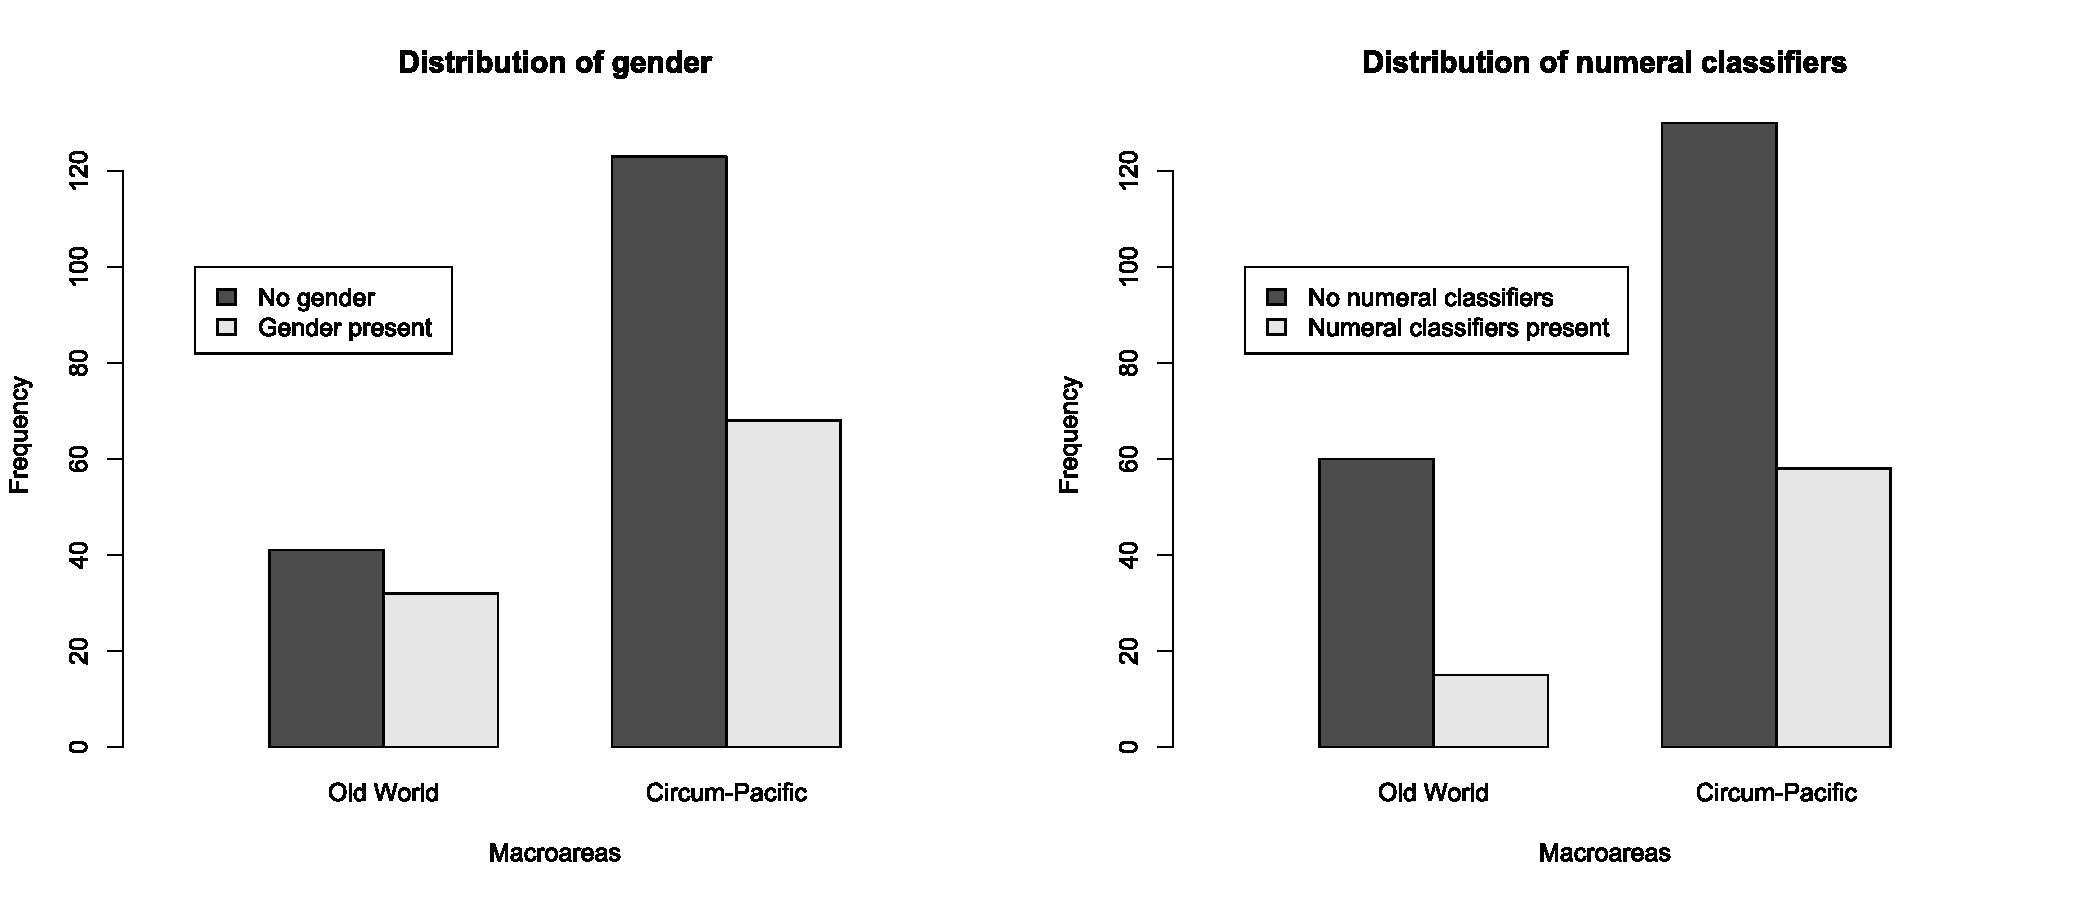
\includegraphics[width=\textwidth]{figures/13/Fig6_barplots}
\caption{Barplots of gender (on the left) and numeral classifiers (on the right) inside and outside the Circum-Pacific region (counts in genera)}
\label{fig:Sinne:6}
\end{figure}

Another possibility is to assume that the probability of developing gender from case or number agreement was roughly similar in the Circum-Pacific and in the Old World. The higher frequency of gender in the Old World could then only be explained by gender being developed more likely from classifiers in the Old World compared to the Circum-Pacific. This explanation could account for the higher than expected frequency of gender in the Old World and also the lower than expected frequency of numeral classifiers in the Old World \textendash{} provided that we assume that when a numeral classifiers system changes into gender that change is complete and the old system of numeral classifiers is practically lost.

This possibility crucially depends on the hypothesized grammaticalization path from classifiers to gender (see \sectref{sec:Sinne:3.2}). Although many researchers have suggested this path as one possibility for gender to develop, \citet[346]{Passer2016b} found no evidence for this process in his in-depth study. He suggests that the reason for the lack of evidence may be the following: when a classifier system turns into a gender system, this change requires large changes in the grammar of the language that go beyond noun classification, including the development of obligatory inflectional agreement. Such large changes in grammars would require that many languages change their morphological type in the process. Numeral classifiers tend to occur especially in analytic languages, but changing morphological type to synthetic is unlikely and rare in the languages of the world. The reasons for the biased areal distributions must, therefore, be sought from elsewhere. (\citealt{Passer2016b}.)

Another reason for the biased areal distributions of gender and numeral classifiers may be related to structural stability (cf.\ \sectref{sec:Sinne:4.1} and \citealt[196--202]{Dahl2004}). Gender and numeral classifiers may simply be stable over very long periods of time, numeral classifiers being further reinforced by neighboring languages in the Circum-Pacific area and gender being reinforced by neighboring languages outside this area. This may be part of the story, since these variables are not the only ones that mark off Circum-Pacific area from the rest of the world. \citet{Bickel2006} show that this area is typologically marked off from the rest of the world by about 40\% of the 86 linguistic variables they surveyed. In addition, \citet[13]{Dediu2013} observed that both gender and numeral classifiers are among the more stable features when compared to the other selected \textit{WALS} features. This stability may be related to language type, as was implied above: although the morphological type of languages may sometimes change, it is unlikely that so extensive changes would be mere epiphenomena of changes in noun classification. Languages are more likely to stick to their morphological type and change some aspects of their linguistic patterns or lose those patterns but not change those patterns completely from one type to another \citep[346]{Passer2016b}. It is more cautious but probably more to the points to say that the kind of noun classification attracted by analytic/isolating languages is (numeral) classifiers and those attracted by languages with inflection is gender (cf. \citealt[137]{Corbett1991}).


\section{Conclusion}
\label{sec:Sinne:6}

In this paper I have researched the interaction between gender and numeral classifiers in a representative sample of the world's languages. The data suggested that there is a strong inverse relationship between gender and numeral classifiers.

This interaction adds to our knowledge of statistical language universals and bespeaks for the existence of complexity trade-offs in well-circumscribed areas of grammar. Previous research has not revealed many instances of complexity trade-offs (e.g., \citealt{Shosted2006}; \citealt{Maddieson2006}; \citealt{Miestamo2009}). Those that have been found, such as the one between case marking and rigid word order (\citealt{Siewierska1998}; \citealt{Sinnemaeki2008}, \citealt{Sinnemaeki2011}, \citealt{Sinnemaeki2014}), have overwhelmingly occurred between functionally related variables that, for instance, tread the same functional domain (such as argument marking). It is possible that new complexity trade-offs will be found among typological variables, but my contention is that they will be found among variables that are functionally related and may therefore also be diachronically connected to one another.

Although the current data suggests a new complexity trade-off this result does not provide evidence for the claim that all languages are equally complex. As I have demonstrated elsewhere (\citealt{Sinnemaeki2014a}) correlational evidence based on typological feature-data cannot either validate or falsify this claim.

I have said very little about the typological distribution of noun classifiers and possessive classifiers. Numeral classifiers are just one subtype of classifiers, so to form a more precise picture of how gender interacts with classifiers in general it would be necessary to survey at least these two types of classifiers in the future as well.

\section*{Acknowledgments}

I would like to thank the audiences of the workshops \textit{Grammatical gender and linguistic complexity} held at the University of Stockholm 20--21 November 2015 and \textit{Gender and Classifiers: Diachronic and Synchronic Variation} at the University of Surrey 28--29 January 2016 for helpful comments. I especially thank Jenny Audring, Greville Corbett, Marcin Kilarski, Don Killian, Johanna Nichols, Maria Polinsky, Adam Schembri, and Marc Tang for their comments. I am grateful to Richard Futrell and Sean Roberts for advice with mixed effects modeling. For financial support I am grateful to the Helsinki Collegium for Advanced Studies and to the Academy of Finland (grant no.~296212).

\section*{Abbreviations}

The following is the list of abbreviations used in the interlinear glosses in this paper:
\medskip

\begin{tabular}{llllll}
\textsc{3}	&	third person	&	\textsc{hum}	&	human	&	\textsc{pl}	&	plural	\\
\textsc{a}	&	active	&	\textsc{icmp}	&	incompletive	&	\textsc{poss}	&	possessor marking	\\
\textsc{anim}	&	animate	&	\textsc{indf}	&	indefinite	&	\textsc{prep}	&	preposition	\\
\textsc{ben}	&	benefactive	&	\textsc{m}	&	masculine	&	\textsc{prf}	&	perfect	\\
\textsc{clf}	&	classifier	&	\textsc{loc}	&	locative	&	\textsc{prox}	&	proximal	\\
\textsc{clt}	&	clitic	&	\textsc{nhum}	&	non-human	&	\textsc{pst}	&	past	\\
\textsc{det}	&	determiner	&	\textsc{nom}	&	nominative	&	\textsc{ref}	&	referential	\\
\textsc{f}	&	feminine	&	\textsc{num}	&	numeral	&	\textsc{sbj}	&	subject	\\
\textsc{fin}	&	finite	&	\textsc{nvis}	&	non-visible	&	\textsc{sg}	&	singular	\\
\textsc{gen}	&	genitive	&	\textsc{obj}	&	object	&	\textsc{wk}	&	week	\\

\end{tabular}


\section*{Appendix 1: Supporting material about mixed effects modeling}

The results of the mixed effect modeling indicated that gender correlated inversely with numeral classifiers irrespective of variation related to language families and geographical areas. Here I discuss the model specifications in greater detail and present also a few additional tests that replicate the results.

One important issue that often surfaces in relation to generalized mixed effects modeling is the convergence of models. A common problem in fitting the models is that they do not always converge. In generalized linear mixed effects modeling an iterative algorithm is used to produce the model parameters. This iteration stops when the difference between successive iterations is smaller than a predetermined tolerance. If so, the model is said to converge, otherwise it is said not to converge. In R the tolerance is set to 1e${-8}$ by default, which means that in practice the model fit cannot be improved with further iterations. See (\citealt[2, 9, 10, 31]{Hardin2007}) and (\citealt[3--4]{Kimballsubmitted}) for more details and references to more technical papers.

When the model does not converge, there are three options available: simplify the models, increase the number of iterations, or use a different optimizer. Based on my experience with generalized linear mixed models using binomial response factors it is hardly ever the case that increasing the number of iterations leads to convergence. The most common alternative in linguistics has been to simplify the models and remove one or more of the random slopes (or the correlation parameters between the random intercept and random slope for some effect). However, there is ongoing debate among researchers whether it is justified to leave out any aspect of the random structure. The simulations of \citet{Barr2013} suggest that it is best to work with maximal models, whereas, for instance, \citet{Baayen2008a}, \citet[395]{Baayen2008}, \citet{Bates2015a}, and \citet{Gries2015} argue that it is fully justified to ask whether all of the random structure is necessary. The statistical literature, on the other hand, suggests that estimating random effects with likelihood ratio test (anova) is not a valid approach for building mixed effects models (see \citealt[8]{Kimballsubmitted} and references there). For this latter reason I did not use model simplification for the purpose of improving convergence. (\citealt{Kimballsubmitted}.)

However, there are situations that may be somewhat problematic if maximal random structure is used. Sometimes the correlation parameter between the random intercept and the random slope for a particular effect is close to or even equals $\pm1.0$. This circumstance means that there is not enough data to fit both a random intercept and a random slope for a particular effect (\citealt{Baayen2008}; \citealt{Bates2015a}). In these situations I followed the recommendations of \citet{Barr2013} and chose to keep the maximal model. There are two reasons for this. First, simplifying the models by removing the correlation between random effects or by removing a random slope usually only increases the likelihood ratio of the fixed term (here numeral classifiers) and makes its p-value smaller. In all the models below, the fixed effect was significant even with the maximal model, so simplifying the models would not have changed the situation. Second, since languages change at different rates across families and areas (cf.\ \citealt{Nichols2003}), it is crucial to include random slopes for both families and areas. Yet owing to the high number of families it may not be usually possible to include more than one random factor for genealogical affiliation especially in Generalized Linear Mixed Models. For instance, \citet{Atkinson2011} modeled both genera and families as random factors but only as random intercepts not as random slopes (or as nested factors, which could have been done). Thus mixed models may not be able to account for the internal structure of language families for which other approaches are called for, such as the Family Bias Theory of \citet{Bickel2013b} or phylogenetic regression (e.g., \citealt{Dunn2011}).

\begin{figure}
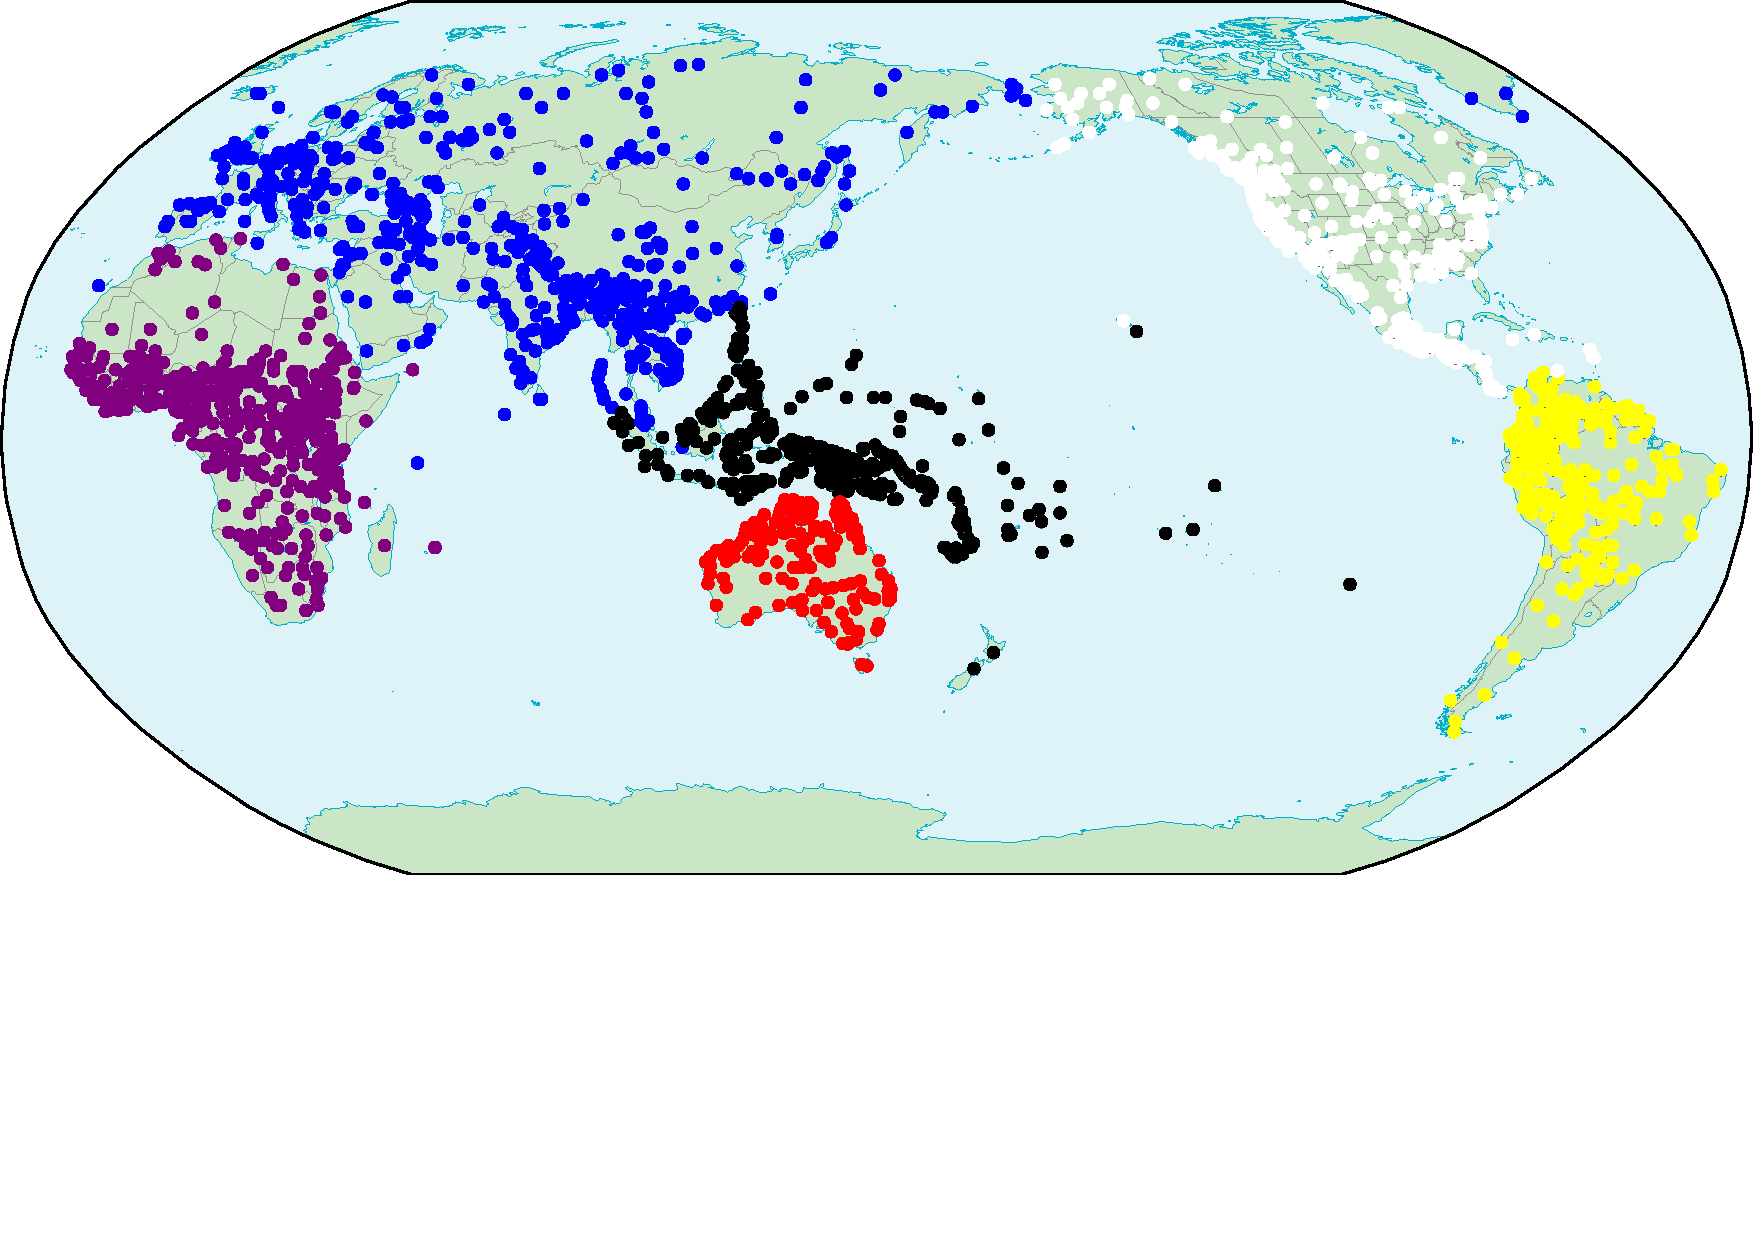
\includegraphics[width=\textwidth]{figures/13/Fig7_Map6areas_s}
\caption{Six macroareas of the \textit{WALS} on the world map}
\label{fig:Sinne:7}
\end{figure}

\begin{figure}
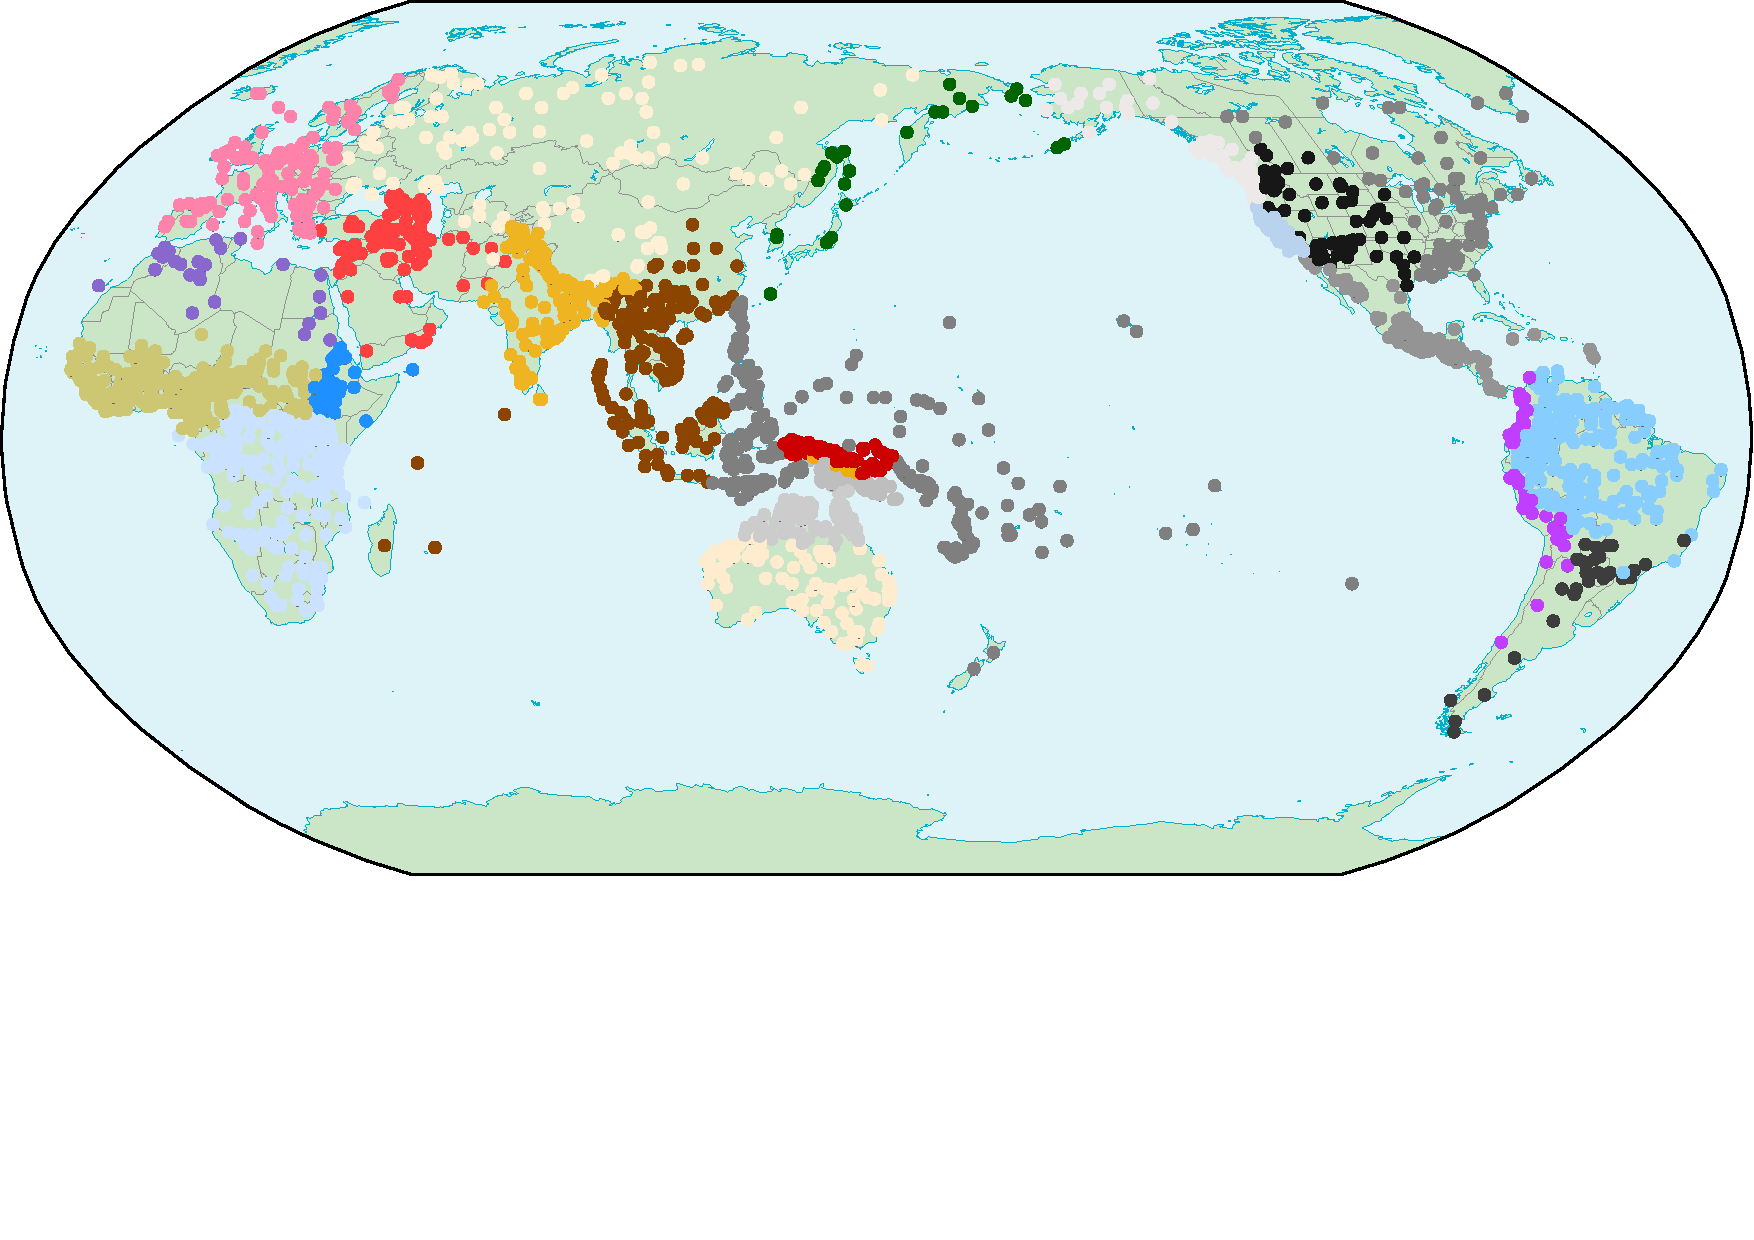
\includegraphics[width=\textwidth]{figures/13/Fig8_Map24areas_s}
\caption{The 24 areas of the \textit{Autotyp} on a world map}
\label{fig:Sinne:8}
\end{figure}

Convergence can be improved also by using a different optimizer. The R package \texttt{lme4} \citep{Bates2015} uses two optimizers, BOBYQA and Nelder-Mead, to estimate the random effects in generalized linear mixed effects modeling. My models did not always converge with the default settings, that is, when using both these optimizers. My solution was to use only one optimizer at a time. I used BOBYQA for most of the models (it is also faster in practice) and Nelder-Mead only when using BOBYQA did not work: these choices resulted in model convergence in all situations. A more general solution to the convergence error is offered by Bayesian mixed effects modeling (see e.g.\ \citealt{Kimballsubmitted}), but I chose to use the frequentist approach here because of its greater familiarity in linguistics.

In the mixed effects modeling I let the intercepts and the slopes vary between the \textit{WALS} families and between the continents as defined in the \textit{Autotyp}. But there are other genealogical classifications that could have been used and the world can also be divided into geographical areas based on different criteria. The classifications I chose capture variation at one particular level of configuration, so it is informative to try out alternative configurations as well. For instance, the ten continents used in the \textit{Autotyp} may conceal variation that occurs in finer-grained areas or in larger macro-areas. For this reason I retested the hypothesis by using an alternative genealogical classification as well as two alternative areal configurations. As an alternative genealogical classification I used stocks, the highest level of classification in the \textit{Autotyp} database \citep{Bickel2017}. As alternative areal configurations I used the six macroareas in the \textit{WALS}, the 24 areas in the \textit{Autotyp}, and the Circum-Pacific vs.\ the Old World as discussed in \sectref{sec:Sinne:4.1}. The six macroareas of the \textit{WALS} are illustrated on a world map in \figref{fig:Sinne:7} (using the 2679 languages of that database), the 24 areas of the \textit{Autotyp} are illustrated in \figref{fig:Sinne:8} (using 2949 languages of that database), and the Circum-Pacific vs.\ the Old World are illustrated in \figref{fig:Sinne:4} in \sectref{sec:Sinne:4.1} (using the languages of my sample).%
\footnote{See \citealt{Hammarstroem2014} for a macroareal definition that is different from those used in the \textit{WALS}. Most areal breakdowns in language typology are based on geography, but it would be possible to use also areal breakdowns based on other criteria, such as social structure \citep{Burton1996}. However, typological research has yet to discuss and employ such approaches.} These combinations of the genealogical and areal classifications produced seven additional models listed in \tabref{tab:Sinne:4}.

\begin{table}[htb]
\footnotesize
\begin{tabularx}{\textwidth}{lXXXrr}
\lsptoprule
\bfseries Model & {\bfseries Areal}

\bfseries configuration & {\bfseries Genealogical}

\bfseries classification & {\bfseries logit \linebreak estimates}

\bfseries + std error & \bfseries $\chi^2$ (1) & \bfseries p-value\\
\midrule
W24 & 24 areas & \textit{WALS}{}-families & $-2.1 \pm 1.1$ & 9.3 & 0.002\\
W6 & 6 macroareas & \textit{WALS}{}-families & $-1.9 \pm 0.9$ & 4.1 & 0.042\\
W2 & Circum-Pacific / Old World & \textit{WALS}{}-families & $-2.0 \pm 0.8$ & 6.3 & 0.012\\
A10 & 10 continents & \textit{Autotyp}{}-stocks & $-3.4 \pm 2.4$ & 8.3 & 0.004\\
A24 & 24 areas & \textit{Autotyp}{}-stocks & $-3.1 \pm 2.3$ & 9.2 & 0.002\\
A6 & 6 macroareas & \textit{Autotyp}{}-stocks & $-3.1 \pm 1.9$ & 4.7 & 0.030\\
A2 & Circum-Pacific / Old World & \textit{Autotyp}{}-stocks & $-5.1 \pm 2.8$ & 8.0 & 0.005\\
\lspbottomrule
\end{tabularx}
\caption{Seven additional models, the design of their random effect structure, and the results of the mixed effects modeling}
\label{tab:Sinne:4}
\end{table}

The results of these additional models are summarized in \tabref{tab:Sinne:4}. As the fourth column suggests, in all the additional models there was an inverse relationship between gender and numeral classifiers. As the rightmost column suggests, this relationship was significant in all the models. These results further replicate those reported in \sectref{sec:Sinne:4.2}.


\section*{Appendix 2: The sample and sources}

The table below provides information about the 360 sample languages, including genealogical classification, macroareal classification, the data on numeral classifiers and gender, and sources. A more detailed database on noun gender is in preparation to \textit{Journal of Cross-Linguistic Databases}.


\begin{landscape}
\tiny
\begin{longtable}{l>{\raggedright\arraybackslash}p{2.2cm}>{\raggedright}p{2.5cm}>{\raggedright\arraybackslash}p{2.5cm}cc>{\raggedright\arraybackslash}p{3.4cm}>{\raggedright\arraybackslash}p{3.4cm}}
\caption{}\\
\lsptoprule Macroarea &  Family &  Genus &  Language &  Cl &  Gd &  Sources (classifiers) &  Sources (gender)\\\midrule\endfirsthead
\midrule    Macroarea &  Family &  Genus &  Language &  Cl &  Gd &  Sources (classifiers) &  Sources (gender)\\\midrule\endhead
\endfoot\lspbottomrule\endlastfoot
Africa & \ili{Afro-Asiatic} & \ili{Berber} & \ili{Berber} (Middle Atlas) & $-$ & $+$ & \citealt[24--25]{Penchoen1973} & \citealt[12--13, 21--22, 25--27, 39--40, 54--55]{Penchoen1973}\\
Africa & \ili{Afro-Asiatic} & \ili{Biu-Mandara} & \ili{Margi} & $-$ & $-$ & \citealt{Gil2013} & \citealt[46, 72--75, 85--87]{Hoffman1963}\\
Africa & \ili{Afro-Asiatic} & Central \ili{Cushitic} & \ili{Kemant} & $-$ & $+$ & \citealt[329]{Appleyard1975}, passim & \citealt[319--322, 332--333]{Appleyard1975}\\
Africa & \ili{Afro-Asiatic} & Dizoid & \ili{Dizi} & $-$ & $+$ & \citealt{Gil2013} & \citealt{Corbett2013}; \citealt[295]{Nichols1992}\\
Africa & \ili{Afro-Asiatic} & E.~\ili{Cushitic} & \ili{Arbore} & $-$ & $+$ & \citealt{Gil2013} & \citealt{Corbett2013}; \citealt[131--132]{Hayward1984}\\
Africa & \ili{Afro-Asiatic} & E.~\ili{Cushitic} & \ili{Oromo (Harar)} & $-$ & $+$ & \citealt{Gil2013} & \citealt{Corbett2013}; \citealt[65]{Owens1985}\\
Africa & \ili{Afro-Asiatic} & E.~\ili{Cushitic} & \ili{Qafar} & $-$ & $+$ & \citealt[185--186]{Bliese1981} & \citealt[180--182, 186--188]{Bliese1981}\\
Africa & \ili{Afro-Asiatic} & S.~\ili{Cushitic} & \ili{Alagwa} & $-$ & $+$ & \citealt{Gil2013} & \citealt{Corbett2013}; \citealt[147--149]{Mous2008}\\
Africa & \ili{Afro-Asiatic} & S.~\ili{Cushitic} & \ili{Iraqw} & $-$ & $+$ & \citealt{Gil2013} & \citealt{Corbett2013}; \citealt[41]{Mous1992}\\
Africa & \ili{Afro-Asiatic} & \ili{Semitic} & \ili{Amharic} & $-$ & $+$ & \citealt{Gil2013} & \citealt{Corbett2013}; \citealt[33--34]{Leslau1995}\\
Africa & \ili{Afro-Asiatic} & \ili{Semitic} & \ili{Arabic (Egyptian)} & $-$ & $+$ & \citealt{Gil2013} & \citealt{Corbett2013}; \citealt[12--18]{Hanna1967}\\
Africa & \ili{Afro-Asiatic} & \ili{Semitic} & \ili{Arabic (Moroccan)} & $-$ & $+$ & \citealt{Gil2013} & \citealt[40, 45--46, 95--97]{Harrell1962}\\
Africa & \ili{Afro-Asiatic} & \ili{Semitic} & \ili{Tigr\'{e}} & $-$ & $+$ & \citealt[110--112]{Elias2005}& \citealt{Corbett2013}; \citealt[210--216]{Elias2005}\\
Africa & \ili{Afro-Asiatic} & W.~\ili{Chadic} & \ili{Hausa} & $-$ & $+$ & \citealt{Gil2013} & \citealt{Corbett2013}; \citealt[47]{Schuh1976}\\
Africa & \ili{Afro-Asiatic} & W.~\ili{Chadic} & \ili{Miya} & $-$ & $+$ & \citealt{Gil2013} & \citealt{Corbett2013}; \citealt[171--173]{Schuh1989}\\
Africa & \ili{Austronesian} & \ili{Barito} & \ili{Malagasy} & $-$ & $-$ & \citealt{Gil2013} & \citealt{Corbett2013}\\
Africa & Central \ili{Sudanic} & \ili{Moru-Ma'di} & \ili{Lugbara} & $-$ & $-$ & \citealt{Gil2013} & \citealt[295]{Nichols1992}\\
Africa & Eastern \ili{Sudanic} & \ili{Kuliak} & \ili{So} & $+$ & $-$ & \citealt{Gil2013} & \citealt[73]{Carlin1993}\\
Africa & Eastern \ili{Sudanic} & \ili{Nilotic} & \ili{Datooga} & $-$ & $-$ & \citealt{Gil2013} & \citealt[passim]{Kiessling2007}\\
Africa & Eastern \ili{Sudanic} & \ili{Nilotic} & \ili{Lango} & $-$ & $-$ & \citealt{Gil2013} & \citealt{Corbett2013}\\
Africa & Eastern \ili{Sudanic} & \ili{Nilotic} & \ili{Maasai} & $-$ & $+$ & \citealt{Gil2013} & \citealt[160]{Payne1998}\\
Africa & Eastern \ili{Sudanic} & \ili{Nubian} & \ili{Nubian (Dongolese)} & $-$ & $-$ & \citealt{Gil2013} & \citealt{Corbett2013}\\
Africa & Eastern \ili{Sudanic} & \ili{Surmic} & \ili{Murle} & $-$ & $-$ & \citealt[100]{Arensen1982}& \citealt{Corbett2013}\\
Africa & \ili{Fur} & \ili{Fur} & \ili{Fur} & $-$ & $+$ & \citealt{Gil2013} & \citealt[84, 99--115]{Jakobi1990}\\
Africa & \ili{Gumuz} & \ili{Gumuz} & \ili{Gumuz} & $-$ & $-$ & \citealt[131--135]{Ahland2012}& \citealt[95--96]{Ahland2012}\\
Africa & \ili{Hadza} & \ili{Hadza} & \ili{Hadza} & $-$ & $+$ & \citealt[passim]{Edenmyr2004} & \citealt[108--110]{Sands2013}\\
Africa & \ili{Kadu} & \ili{Kadugli} & \ili{Krongo} & $-$ & $+$ & \citealt[309--310]{Reh1985}& \citealt[126--127]{Reh1985}\\
Africa & \ili{Khoe-Kwadi} & \ili{Khoe-Kwadi} & \ili{Khoekhoe} & $-$ & $+$ & \citealt{Gil2013} & \citealt{Corbett2013}; \citealt[81--88]{Hagman1973}\\
Africa & \ili{Koman} & \ili{Koman} & \ili{Uduk} & $-$ & $+$ & \citealt[129--132]{Killian2015}& \citealt[67--68]{Killian2015}\\
Africa & \ili{Kordofanian} & \ili{Rashad} & \ili{Orig} & $-$ & $+$ & \citealt{Gil2013} & \citealt[295]{Nichols1992}\\
Africa & \ili{Kx'a} & \ili{Ju Kung} & \ili{Juǀ’hoan} & $-$ & $-$ & \citealt{Gil2013} & \citealt{Corbett2013}; \citealt[12--16]{Dickens1992}\\
Africa & \ili{Mande} & W.~Mande & \ili{Mandinka} (Gambian) & $-$ & $-$ & \citealt[295]{Nichols1992}& \citealt[295]{Nichols1992}\\
Africa & \ili{Niger-Congo} & \ili{Bantoid} & \ili{Ejagham} & $+$ & $+$ & \citealt[309--313]{Watters1981}& \citealt[291--293, 318--321, 328--331, 434--440]{Watters1981}\\
Africa & \ili{Niger-Congo} & \ili{Bantoid} & \ili{Lingala} & $-$ & $+$ & \citealt[23--24]{Meeuwis1998}& \citealt{Corbett2013}; \citealt[110--111]{Kamwangamalu1989}\\
Africa & \ili{Niger-Congo} & \ili{Bantoid} & \ili{Luganda} & $-$ & $+$ & \citealt{Gil2013} & \citealt[295]{Nichols1992}\\
Africa & \ili{Niger-Congo} & \ili{Bantoid} & \ili{Luvale} & $-$ & $+$ & \citealt[36--37, 166--167]{Horton1949} & \citealt[36--37, 166--167]{Horton1949}\\
Africa & \ili{Niger-Congo} & \ili{Bantoid} & \ili{Shona} & $-$ & $+$ & \citealt[108--109, 127]{Fortune1985} & \citealt{Corbett2013}; \citealt[107--126]{Fortune1985}\\
Africa & \ili{Niger-Congo} & \ili{Bantoid} & \ili{Swahili} & $-$ & $+$ & \citealt{Gil2013} & \citealt{Corbett2013}; own knowledge\\
Africa & \ili{Niger-Congo} & \ili{Bantoid} & \ili{Zulu} & $-$ & $+$ & \citealt{Gil2013} & \citealt{Corbett2013}; \citealt[21]{Canonici1995}\\
Africa & \ili{Niger-Congo} & \ili{Cross River} & \ili{Kana} & $+$ & $-$ & \citealt{Gil2013} & \citealt[110--111]{Aikhenvald2000}\\
Africa & \ili{Niger-Congo} & \ili{Defoid} & \ili{Yoruba} & $-$ & $-$ & \citealt{Gil2013} & \citealt{Corbett2013}\\
Africa & \ili{Niger-Congo} & \ili{Gbaya-Manza-Ngbaka} & \ili{Gbeya Bossangoa} & $-$ & $-$ & \citealt{Gil2013} & \citealt[98]{Samarin1966}\\
Africa & \ili{Niger-Congo} & \ili{Gur} & \ili{Dagaare} & $-$ & $+$ & \citealt{Gil2013} & \citealt[45--48]{Grimm2012}\\
Africa & \ili{Niger-Congo} & \ili{Gur} & \ili{Koromfe} & $-$ & $+$ & \citealt{Gil2013} & \citealt{Corbett2013}; \citealt[206--233]{Rennison1997}\\
Africa & \ili{Niger-Congo} & \ili{Gur} & \ili{Supyire} & $-$ & $+$ & \citealt{Gil2013} & \citealt{Corbett2013}; \citealt[75]{Carlson1994}\\
Africa & \ili{Niger-Congo} & Igboid & \ili{Igbo} & $-$ & $-$ & \citealt{Gil2013} & \citealt{Corbett2013}\\
Africa & \ili{Niger-Congo} & N.~\ili{Atlantic} & \ili{Diola-Fogny} & $-$ & $+$ & \citealt[74]{Sapir1965}& \citealt[24--25, 61--62]{Sapir1965}\\
Africa & \ili{Niger-Congo} & N.~\ili{Atlantic} & \ili{Fula} (Cameroonian) & $+$ & $+$ & \citealt[295]{Nichols1992}& \citealt[295]{Nichols1992}\\
Africa & \ili{Niger-Congo} & \ili{Ubangi} & \ili{Zande} & $-$ & $-$ & \citealt[42--45]{Gore1926}& \citealt{Corbett2013}; \citealt[20--23]{Gore1926}\\
Africa & \ili{Saharan} & W.~Saharan & \ili{Kanuri} & $-$ & $-$ & \citealt{Gil2013} & \citealt{Corbett2013}\\
Africa & \ili{Sandawe} & \ili{Sandawe} & \ili{Sandawe} & $-$ & $+$ & \citealt{Gil2013} & \citealt[295]{Nichols1992}; \citealt[14--17]{Eaton2010}\\
Africa & \ili{Songhay} & Songhay & \ili{Koyra Chiini} & $-$ & $-$ & \citealt{Gil2013} & \citealt[55]{Heath1999}\\
Australia & \ili{Bunuban} & Bunuban & \ili{Gooniyandi} & $-$ & $-$ & \citealt{Gil2013} & \citealt{Corbett2013}\\
Australia & \ili{Gaagudju} & \ili{Gaagudju} & \ili{Gaagudju} & $-$ & $+$ & \citealt{Gil2013} & \citealt[144--157]{Harvey2002}\\
Australia & Garrwan & Garrwan & \ili{Garrwa} & $-$ & $-$ & \citealt{Gil2013} & \citealt[38, 190]{Mushin2012}\\
Australia & \ili{Gunwinyguan} & \ili{Nunggubuyu} & \ili{Nunggubuyu} & $-$ & $+$ & \citealt{Gil2013} & \citealt{Corbett2013}; \citealt[131--132]{Heath1983}\\
Australia & \ili{Iwaidjan} & Iwaidjan & \ili{Mawng} & $-$ & $+$ & \citealt{Gil2013} & \citealt{Corbett2013}; \citealt[73--77]{Capell1970}\\
Australia & \ili{Mangarrayi-Maran} & \ili{Alawa} & \ili{Alawa} & $-$ & $+$ & \citealt[passim]{Sharpe1972} & \citealt[66, 79--80]{Sharpe1972}\\
Australia & \ili{Mangarrayi-Maran} & \ili{Mangarrayi} & \ili{Mangarrayi} & $-$ & $+$ & \citealt{Gil2013} & \citealt{Corbett2013}; \citealt[297]{Nichols1992}\\
Australia & \ili{Mangarrayi-Maran} & \ili{Warndarang} & \ili{Warndarang} & $-$ & $+$ & \citealt{Gil2013} & \citealt[299]{Nichols1992}; \citealt[22--23]{Heath1980}\\
Australia & \ili{Mirndi} & \ili{Djingili} & \ili{Djingili} & $-$ & $+$ & \citealt{Gil2013} & \citealt[247--248, 253--259]{Pensalfini1997}\\
Australia & Mirndi & Jaminjungan & \ili{Jaminjung} & $-$ & $-$ & \citealt{Gil2013} & \citealt[passim]{Schultze-Berndt2000}\\
Australia & Mirndi & Wambayan & \ili{Wambaya} & $-$ & $+$ & \citealt[72--80]{Nordlinger1998}& \citealt[59--70]{Nordlinger1998}\\
Australia & N.~Daly\il{Northern Daly} & N.~Daly & \ili{Malakmalak} & $-$ & $+$ & \citealt{Gil2013} & \citealt[30--31]{Birk1976}\\
Australia & \ili{Pama-Nyungan} & N.~\ili{Pama-Nyungan} & \ili{Dyirbal} & $-$ & $+$ & \citealt{Gil2013} & \citealt{Corbett2013}; \citealt[44]{Dixon1972}\\
Australia & \ili{Pama-Nyungan} & N.~\ili{Pama-Nyungan} & \ili{Uradhi} & $-$ & $-$ & \citealt{Gil2013} & \citealt{Corbett2013}\\
Australia & \ili{Pama-Nyungan} & N.~\ili{Pama-Nyungan} & Yidiny\il{Yidiñ} & $-$ & $-$ & \citealt{Gil2013} & \citealt{Corbett2013}\\
Australia & \ili{Pama-Nyungan} & S.-E.~\ili{Pama-Nyungan} & \ili{Ngiyambaa} & $-$ & $-$ & \citealt{Gil2013} & \citealt{Corbett2013}\\
Australia & \ili{Pama-Nyungan} & W.~\ili{Pama-Nyungan} & \ili{Martuthunira} & $-$ & $-$ & \citealt{Gil2013} & \citealt{Corbett2013}\\
Australia & \ili{Pama-Nyungan} & W.~\ili{Pama-Nyungan} & \ili{Yingkarta} & $-$ & $-$ & \citealt{Gil2013} & \citealt[20]{Dench1998}\\
Australia & Tiwian & Tiwian & \ili{Tiwi} & $-$ & $+$ & \citealt{Gil2013} & \citealt{Corbett2013}; \citealt[51--52]{Osborne1974}\\
Australia & \ili{Worrorran} & Worrorran & \ili{Gunin} & $-$ & $+$ & \citealt{Gil2013} & \citealt[146--149]{McGregor2004}\\
Australia & Worrorran & Worrorran & \ili{Ungarinjin} & $-$ & $-$ & \citealt{Gil2013} & \citealt[299]{Nichols1992}\\
Australia & Worrorran & Worrorran & \ili{Worora} & $-$ & $+$ & \citealt{Gil2013} & \citealt[95]{Clendon2000}\\
Australia & \ili{Yangmanic} & Yangmanic & \ili{Wardaman} & $-$ & $+$ & \citealt[120]{Merlan1994}& \citealt{Corbett2013}; \citealt[61--63, 241--242]{Merlan1994}\\
Eurasia & \ili{Afro-Asiatic} & \ili{Semitic} & \ili{Hebrew} (Modern) & $-$ & $+$ & \citealt{Gil2013} & \citealt{Corbett2013}; \citealt[51--52, 91, 104, 117--120, 185--198]{Glinert1989}\\
Eurasia & \ili{Ainu} & \ili{Ainu} & \ili{Ainu} & $+$ & $-$ & \citealt{Gil2013} & \citealt{Corbett2013}\\
Eurasia & \ili{Altaic} & \ili{Mongolic} & \ili{Buriat} & $-$ & $-$ & \citealt{Gil2013} & \citealt[110--111, 117--120]{Skribnik2003}\\
Eurasia & \ili{Altaic} & Mongolic & \ili{Khalkha} & $-$ & $-$ & \citealt{Gil2013} & \citealt{Corbett2013}\\
Eurasia & \ili{Altaic} & \ili{Tungusic} & \ili{Evenki} & $-$ & $-$ & \citealt{Gil2013} & \citealt{Corbett2013}\\
Eurasia & \ili{Altaic} & Tungusic & \ili{Nanai} & $-$ & $-$ & \citealt{Gil2013} & \citealt[297]{Nichols1992}\\
Eurasia & \ili{Altaic} & \ili{Turkic} & \ili{Chuvash} & $-$ & $-$ & \citealt{Gil2013} & \citealt{Corbett2013}\\
Eurasia & \ili{Altaic} & \ili{Turkic} & \ili{Tatar} & $+$ & $-$ & \citealt{Gil2013} & \citealt[29--57]{Poppe1968}\\
Eurasia & \ili{Altaic} & \ili{Turkic} & \ili{Turkish} & $+$ & $-$ & \citealt{Gil2013} & \citealt{Corbett2013}\\
Eurasia & \ili{Altaic} & \ili{Turkic} & \ili{Tuvan} & $-$ & $-$ & \citealt{Gil2013} & \citealt[297]{Nichols1992}\\
Eurasia & \ili{Austroasiatic} & \ili{Aslian} & \ili{Semelai} & $+$ & $-$ & \citealt{Gil2013} & \citealt{Corbett2013}\\
Eurasia & \ili{Austroasiatic} & \ili{Khasian} & \ili{Pnar} & $+$ & $+$ & \citealt[124--125, 357--369]{Ring2015} & \citealt[101, 107--108]{Ring2015}\\
Eurasia & \ili{Austroasiatic} & \ili{Khmer} & \ili{Khmer} & $+$ & $-$ & \citealt{Gil2013} & \citealt{Corbett2013}\\
Eurasia & \ili{Austroasiatic} & \ili{Munda} & \ili{Korku} & $-$ & $+$ & \citealt{Gil2013} & \citealt[passim]{Bhattacharya1976}\\
Eurasia & \ili{Austroasiatic} & Munda & \ili{Santali} & $+$ & $+$ & \citealt{Gil2013} & \citealt[11--12, 32--33, 39--40, 44--45]{Ghosh2008}\\
Eurasia & \ili{Austroasiatic} & \ili{Nicobarese} & \ili{Nicobarese} (Car) & $+$ & $+$ & \citealt{Gil2013} & \citealt{Corbett2013}; \citealt[103--108]{Braine1970}\\
Eurasia & \ili{Austroasiatic} & \ili{Palaung-Khmuic} & \ili{Khmu'} & $+$ & $-$ & \citealt{Gil2013} & \citealt{Corbett2013}; \citealt[30, 32--33]{Premsrirat1987}\\
Eurasia & \ili{Austroasiatic} & \ili{Viet-Muong} & \ili{Vietnamese} & $+$ & $-$ & \citealt{Gil2013} & \citealt{Corbett2013}\\
Eurasia & \ili{Austronesian} & \ili{Malayo-Sumbawan} & \ili{Acehnese} & $+$ & $-$ & \citealt[137--139]{Durie1985}& \citealt[29]{Durie1985}\\
Eurasia & \ili{Austronesian} & Malayo-Sumbawan & \ili{Cham} (E.) & $+$ & $-$ & \citealt{Gil2013} & \citealt[passim]{Thurgood2005}\\
Eurasia & \ili{Basque} & \ili{Basque} & \ili{Basque} & $-$ & $-$ & \citealt{Gil2013} & \citealt{Corbett2013}\\
Eurasia & \ili{Burushaski} & \ili{Burushaski} & \ili{Burushaski} & $-$ & $+$ & \citealt{Gil2013} & \citealt{Corbett2013}; \citealt[161--167]{Munshi2006}\\
Eurasia & \ili{Chukotko-Kamchatkan} & N.~Chukotko-Kamchatkan & \ili{Chukchi} & $-$ & $-$ & \citealt{Gil2013} & \citealt{Corbett2013}\\
Eurasia & \ili{Dravidian} & N.~\ili{Dravidian} & \ili{Brahui} & $-$ & $-$ & \citealt{Gil2013} & \citealt{Corbett2013}\\
Eurasia & \ili{Dravidian} & S.~\ili{Dravidian} & \ili{Kannada} & $-$ & $+$ & \citealt{Gil2013} & \citealt{Corbett2013}; \citealt[221--222]{Sridhar1990}\\
Eurasia & \ili{Dravidian} & S.~\ili{Dravidian} & \ili{Tamil} & $-$ & $+$ & \citealt[48--50]{Schiffman1999}& \citealt{Corbett2013}; \citealt[57--58]{Schiffman1999}\\
Eurasia & Hmong-Mien & \ili{Hmong-Mien} & \ili{Hmong Daw} & $+$ & $-$ & \citealt{Gil2013} & \citealt[297]{Nichols1992}\\
Eurasia & \ili{Indo-European} & \ili{Albanian} & \ili{Albanian} & $-$ & $+$ & \citealt{Gil2013} & \citealt[17, 18, 29]{Matasovic2012a}\\
Eurasia & \ili{Indo-European} & \ili{Armenian} & Armenian (E.) & $-$ & $-$ & \citealt{Gil2013} & \citealt{Corbett2013}\\
Eurasia & \ili{Indo-European} & \ili{Baltic} & \ili{Latvian} & $-$ & $+$ & \citealt{Gil2013} & \citealt{Corbett2013}; \citealt[66--73]{Kalnaca2014}\\
Eurasia & \ili{Indo-European} & \ili{Germanic} & \ili{English} & $-$ & $-$ & \citealt{Gil2013} & \citealt{Corbett2013}; own knowledge\\
Eurasia & \ili{Indo-European} & \ili{Germanic} & \ili{German} & $-$ & $+$ & \citealt{Gil2013} & \citealt{Corbett2013}; own knowledge\\
Eurasia & \ili{Indo-European} & \ili{Indic} & \ili{Assamese} & $+$ & $-$ & \citealt{Gil2013} &  \citealt[415]{Goswami2003}\\
Eurasia & \ili{Indo-European} & \ili{Indic} & \ili{Bengali} & $+$ & $-$ & \citealt{Gil2013} & \citealt[425]{Klaiman2009}\\
Eurasia & \ili{Indo-European} & \ili{Indic} & \ili{Hindi} & $-$ & $+$ & \citealt{Gil2013} & \citealt{Corbett2013}; \citealt[1--22]{McGregor1986}\\
Eurasia & \ili{Indo-European} & \ili{Indic} & \ili{Marathi} & $-$ & $+$ & \citealt{Gil2013} & \citealt{Corbett2013}; \citealt[702--707]{Pandharipande2003}\\
Eurasia & \ili{Indo-European} & \ili{Indic} & \ili{Sinhala} & $-$ & $+$ & \citealt{Gil2013} & \citealt[passim]{Henadeerage2002}; \citealt[79--82, 228--229]{Chandralai2010}\\
Eurasia & \ili{Indo-European} & \ili{Indic} & \ili{Waigali} & $-$ & $+$ & \citealt{Gil2013} & \citealt[297]{Nichols1992}\\
Eurasia & \ili{Indo-European} & \ili{Iranian} & \ili{Persian} & $+$ & $-$ & \citealt{Gil2013} & \citealt{Corbett2013}\\
Eurasia & \ili{Indo-European} & \ili{Romance} & \ili{French} & $-$ & $+$ & \citealt{Gil2013} & \citealt{Corbett2013}; own knowledge\\
Eurasia & \ili{Indo-European} & \ili{Slavic} & \ili{Bulgarian} & $-$ & $+$ & \citealt{Gil2013} & \citealt[86--89]{Nicolova2017}\\
Eurasia & \ili{Indo-European} & \ili{Slavic} & \ili{Russian} & $-$ & $+$ & \citealt{Gil2013} & \citealt{Corbett2013}; \citealt[54]{Wade2011}\\
Eurasia & \ili{Japanese} & \ili{Japanese} & \ili{Japanese} & $+$ & $-$ & \citealt{Gil2013} & \citealt[passim]{Kaiser2001}\\
Eurasia & \ili{Kartvelian} & Kartvelian & \ili{Georgian} & $-$ & $-$ & \citealt{Gil2013} & \citealt{Corbett2013}\\
Eurasia & \ili{Korean} & \ili{Korean} & \ili{Korean} & $+$ & $-$ & \citealt{Gil2013} & \citealt[297]{Nichols1992}\\
Eurasia & \ili{Nakh-Daghestanian} & \ili{Avar-Andic-Tsezic} & \ili{Avar} & $-$ & $+$ & \citealt{Gil2013} & \citealt[29--30]{Charachidze1981}; \citealt[155--156]{Berg2005}\\
Eurasia & \ili{Nakh-Daghestanian} & \ili{Avar-Andic-Tsezic} & \ili{Bagvalal} & $-$ & $+$ & \citealt{Gil2013} & \citealt[749--750]{Corbett2006}\\
Eurasia & \ili{Nakh-Daghestanian} & \ili{Avar-Andic-Tsezic} & \ili{Hunzib} & $-$ & $+$ & \citealt{Gil2013} & \citealt{Corbett2013}; \citealt[1367]{Berg2004}\\
Eurasia & \ili{Nakh-Daghestanian} & \ili{Lak-Dargwa} & \ili{Dargwa} & $-$ & $+$ & \citealt{Gil2013} & \citealt[156--158]{Berg2005}\\
Eurasia & \ili{Nakh-Daghestanian} & \ili{Lezgic} & \ili{Lezgian} & $-$ & $-$ & \citealt{Gil2013} & \citealt{Corbett2013}\\
Eurasia & \ili{Nakh-Daghestanian} & \ili{Nakh} & \ili{Chechen} & $-$ & $+$ & \citealt{Gil2013} & \citealt[37]{Nichols1994}\\
Eurasia & \ili{Nakh-Daghestanian} & \ili{Nakh} & \ili{Ingush} & $-$ & $+$ & \citealt{Gil2013} & \citealt{Corbett2013}; \citealt[141--142]{Nichols2011}\\
Eurasia & \ili{Nivkh} & \ili{Nivkh} & \ili{Nivkh} & $+$ & $-$ & \citealt{Gil2013} & \citealt{Corbett2013}\\
Eurasia & NW Caucasian & NW Caucasian & \ili{Abkhaz} & $-$ & $+$ & \citealt{Gil2013} & \citealt{Corbett2013}; \citealt[108]{Spruit1986}\\
Eurasia & \ili{Sino-Tibetan} & \ili{Bodic} & \ili{Gurung} & $-$ & $-$ & \citealt[297]{Nichols1992}& \citealt[297]{Nichols1992}\\
Eurasia & \ili{Sino-Tibetan} & \ili{Bodo-Garo} & \ili{Garo} & $+$ & $-$ & \citealt{Gil2013} & \citealt[passim]{Burling1961}\\
Eurasia & \ili{Sino-Tibetan} & \ili{Burmese-Lolo} & \ili{Burmese} & $+$ & $-$ & \citealt{Gil2013} & \citealt{Corbett2013}\\
Eurasia & \ili{Sino-Tibetan} & \ili{Burmese-Lolo} & \ili{Lahu} & $+$ & $-$ & \citealt{Gil2013} & \citealt{Corbett2013}\\
Eurasia & \ili{Sino-Tibetan} & \ili{Chinese} & \ili{Cantonese} & $+$ & $-$ & \citealt{Gil2013} & \citealt{Corbett2013}\\
Eurasia & \ili{Sino-Tibetan} & \ili{Chinese} & \ili{Mandarin} & $+$ & $-$ & \citealt{Gil2013} & \citealt{Corbett2013}\\
Eurasia & \ili{Sino-Tibetan} & \ili{Mahakiranti} & \ili{Chepang} & $-$ & $-$ & \citealt{Gil2013} & \citealt[42, 50, 51, 55]{Caughley1982}\\
Eurasia & \ili{Tai-Kadai} & \ili{Kadai} & \ili{Lachi} & $+$ & $-$ & \citealt{Gil2013} & \citealt[68--77]{Kosaka2000}\\
Eurasia & Tai-Kadai & \ili{Kam-Tai} & \ili{Thai} & $+$ & $-$ & \citealt{Gil2013} & \citealt{Corbett2013}\\
Eurasia & \ili{Uralic} & \ili{Finnic} & \ili{Finnish} & $-$ & $-$ & \citealt{Gil2013} & \citealt{Corbett2013}\\
Eurasia & \ili{Uralic} & \ili{Mordvin} & \ili{Mordvin} (Erzya) & $-$ & $-$ & \citealt{Gil2013} & \citealt[191--197]{Zaicz1998}\\
Eurasia & \ili{Uralic} & \ili{Permic} & \ili{Komi-Zyrian} & $-$ & $-$ & \citealt{Gil2013} & \citealt[295]{Nichols1992}\\
Eurasia & \ili{Uralic} & \ili{Samoyedic} & \ili{Nenets} & $-$ & $-$ & \citealt{Gil2013} & \citealt{Corbett2013}\\
Eurasia & \ili{Uralic} & \ili{Ugric} & \ili{Hungarian} & $+$ & $-$ & \citealt{Gil2013} & \citealt{Corbett2013}\\
Eurasia & \ili{Yukaghir} & \ili{Yukaghir} & Yukaghir (Kolyma)\il{Yukaghir, Kolyma} & $-$ & $-$ & \citealt{Gil2013} & \citealt{Corbett2013}\\
N.~America & \ili{Algic} & \ili{Algonquian} & \ili{Cree (Plains)} & $-$ & $+$ & \citealt{Gil2013} & \citealt{Corbett2013}; \citealt[20--24, 33--38]{Wolfart1973}\\
N.~America & \ili{Algic} & \ili{Yurok} & \ili{Yurok} & $+$ & $-$ & \citealt[299]{Nichols1992}& \citealt{Corbett2013}\\
N.~America & \ili{Atakapa} & \ili{Atakapa} & \ili{Atakapa} & $-$ & $-$ & \citealt{Gil2013} & \citealt[125, 136--140]{Swanton1929}\\
N.~America & \ili{Chibchan} & \ili{Talamanca} & \ili{Teribe} & $+$ & $-$ & \citealt{Gil2013} & \citealt[passim]{Quesada2010}\\
N.~America & Chimakuan & \ili{Chimakuan} & \ili{Quileute} & $-$ & $+$ & \citealt{Gil2013} & \citealt[299]{Nichols1992}\\
N.~America & \ili{Chitimacha} & \ili{Chitimacha} & \ili{Chitimacha} & $-$ & $-$ & \citealt{Gil2013} & \citealt[52--53, 78--85]{Granberry2004}\\
N.~America & \ili{Chumash} & \ili{Chumash} & \ili{Chumash} (\ili{Barbareño}) & $-$ & $-$ & \citealt{Gil2013} & \citealt[passim]{Wash2001}\\
N.~America & \ili{Chumash} & \ili{Chumash} & \ili{Chumash} (\ili{Ineseño}) & $-$ & $-$ & \citealt{Gil2013} & \citealt[passim]{Applegate1972}\\
N.~America & \ili{Eskimo-Aleut} & Eskimo & \ili{Yup'ik} (C.) & $-$ & $-$ & \citealt[201--207]{Reed1977}& \citealt{Corbett2013}\\
N.~America & \ili{Haida} & \ili{Haida} & \ili{Haida} & $+$ & $-$ & \citealt{Gil2013} & \citealt{Corbett2013}\\
N.~America & \ili{Hokan} & \ili{Chimariko} & \ili{Chimariko} & $-$ & $-$ & \citealt{Gil2013} & \citealt{Corbett2013}\\
N.~America & Hokan & \ili{Yuman} & \ili{Diegueño (Mesa Grande)} & $-$ & $-$ & \citealt[299]{Nichols1992} & \citealt[299]{Nichols1992}\\
N.~America & Hokan & Yuman & \ili{Maricopa} & $-$ & $-$ & \citealt{Gil2013} & \citealt{Corbett2013}\\
N.~America & \ili{Iroquoian} & N.~\ili{Iroquoian} & \ili{Seneca} & $-$ & $+$ & \citealt{Gil2013} & \citealt{Corbett2013}; \citealt[13--22]{Chafe1967}\\
N.~America & \ili{Karok} & \ili{Karok} & \ili{Karok} & $-$ & $-$ & \citealt{Gil2013} & \citealt{Corbett2013}\\
N.~America & Keresan & \ili{Keresan} & \ili{Acoma} & $-$ & $-$ & \citealt{Gil2013} & \citealt{Corbett2013}\\
N.~America & \ili{Kiowa-Tanoan} & \ili{Kiowa}-Tanoan & \ili{Kiowa} & $-$ & $+$ & \citealt{Gil2013} & \citealt[59--67]{Sutton2010}\\
N.~America & \ili{Kutenai} & \ili{Kutenai} & \ili{Kutenai} & $-$ & $-$ & \citealt{Gil2013} & \citealt{Corbett2013}\\
N.~America & \ili{Mayan} & \ili{Mayan} & \ili{Jacaltec} & $+$ & $-$ & \citealt{Gil2013}; \citealt[244]{Craig1986} & \citealt[passim]{Day1973}\\
N.~America & \ili{Mayan} & \ili{Mayan} & \ili{Tzeltal} & $+$ & $-$ & \citealt{Gil2013} & \citealt[171--172]{Kaufman1963}\\
N.~America & \ili{Mayan} & \ili{Mayan} & \ili{Tzutujil} & $+$ & $-$ & \citealt[301]{Nichols1992} & \citealt[301]{Nichols1992}\\
N.~America & \ili{Mayan} & \ili{Mayan} & \ili{Yucatec} & $+$ & $-$ & \citealt{Gil2013} & \citealt[66, 69]{Brody2004}\\
N.~America & \ili{Misumalpan} & Misumalpan & \ili{Miskito} & $-$ & $-$ & \citealt{Gil2013} & \citealt[56]{Heath1913}\\
N.~America & \ili{Muskogean} & Muskogean & \ili{Choctaw} & $-$ & $-$ & \citealt{Gil2013} & \citealt[passim]{Davies1986}\\
N.~America & \ili{Na-Dene} & \ili{Athapaskan} & \ili{Navajo} & $-$ & $-$ & \citealt{Gil2013} & \citealt[299]{Nichols1992}\\
N.~America & Na-Dene & \ili{Tlingit} & \ili{Tlingit} & $+$ & $-$ & \citealt{Gil2013} & \citealt[passim]{Boas1917}\\
N.~America & \ili{Oregon Coast} & \ili{Coosan} & \ili{Coos (Hanis)} & $-$ & $-$ & \citealt{Gil2013} & \citealt{Corbett2013}\\
N.~America & \ili{Otomanguean} & \ili{Chichimec} & \ili{Chichimeca-Jonaz} & $-$ & $-$ & \citealt{Gil2013} & \citealt[23--30]{Suarez1984}\\
N.~America & \ili{Otomanguean} & \ili{Mixtecan} & Mixtec (Chalcatongo)\il{Mixtec, Chalcatongo} & $-$ & $-$ & \citealt{Gil2013} & \citealt{Corbett2013}; \citealt[81--85]{Macaulay1996}\\
N.~America & \ili{Otomanguean} & \ili{Otomian} & \ili{Otom\'{i}\ (Mezquital)} & $-$ & $-$ & \citealt[passim]{Hess1968} & \citealt[passim]{Hess1968}\\
N.~America & \ili{Otomanguean} & \ili{Zapotecan} & \ili{Zapotec (Coatlán)} & $-$ & $-$ & \citealt[passim]{BeamdeAzcona2004} & \citealt[passim]{BeamdeAzcona2004}\\
N.~America & \ili{Penutian} & Chinookan & \ili{Chinook (Upper)} & $-$ & $+$ & \citealt{Gil2013} & \citealt[72--75, 214]{Hymes1955}\\
N.~America & Penutian & \ili{Klamath-Modoc} & \ili{Klamath} & $-$ & $-$ & \citealt{Gil2013} & \citealt[448--451]{Mithun2001}\\
N.~America & Penutian & Maiduan & \ili{Maidu} (NE) & $-$ & $-$ & \citealt{Gil2013} & \citealt[299]{Nichols1992}\\
N.~America & Penutian & \ili{Miwok} & \ili{Miwok} (S.~Sierra) & $-$ & $-$ & \citealt{Gil2013} & \citealt{Corbett2013}\\
N.~America & Penutian & Sahaptian & \ili{Sahaptin (Umatilla)} & $+$ & $-$ & \citealt[299]{Nichols1992} & \citealt[299]{Nichols1992}\\
N.~America & Penutian & Tsimshianic & \ili{Gitksan} & $+$ & $-$ & \citealt[299]{Nichols1992} & \citealt[passim]{Hunt1993}\\
N.~America & Penutian & Tsimshianic & \ili{Tsimshian} (Coast) & $+$ & $-$ & \citealt{Gil2013} & \citealt{Corbett2013}\\
N.~America & \ili{Penutian} & \ili{Yokuts} & \ili{Yawelmani} & $-$ & $-$ & \citealt{Gil2013} & \citealt[299]{Nichols1992}\\
N.~America & \ili{Salinan} & \ili{Salinan} & \ili{Salinan} & $-$ & $-$ & \citealt{Gil2013} & \citealt[299]{Nichols1992}\\
N.~America & Salishan & Central \ili{Salish} & \ili{Halkomelem} (Island) & $+$ & $+$ & \citealt[254--266]{Gerdts2004} & \citealt[417--418]{Gerdts2013}; \citealt[176--177]{Gerdts2010}\\
N.~America & Salishan & Interior \ili{Salish} & \ili{Thompson} & $+$ & $-$ & \citealt{Gil2013} & \citealt{Corbett2013}\\
N.~America & \ili{Siouan} & Core \ili{Siouan} & \ili{Lakhota} & $-$ & $+$ & \citealt{Gil2013} & \citealt[36--37]{Valin1977}\\
N.~America & \ili{Siouan} & Core \ili{Siouan} & \ili{Mandan} & $-$ & $-$ & \citealt{Gil2013} & \citealt[passim]{Kennard1936}\\
N.~America & \ili{Takelma} & \ili{Takelma} & \ili{Takelma} & $-$ & $-$ & \citealt{Gil2013} & \citealt[299]{Nichols1992}\\
N.~America & Tequistlatecan & \ili{Tequistlatecan} & \ili{Chontal (Huamelultec Oaxaca)} & $-$ & $-$ & \citealt[301]{Nichols1992} & \citealt[356--358]{Waterhouse1967}\\
N.~America & \ili{Tol} & \ili{Tol} & \ili{Tol} & $-$ & $-$ & \citealt{Gil2013} & \citealt{Corbett2013}\\
N.~America & \ili{Totonacan} & \ili{Totonacan} & \ili{Tepehua (Tlachichilco)} & $+$ & $-$ & \citealt[301]{Nichols1992} & \citealt[301]{Nichols1992}\\
N.~America & \ili{Tunica} & \ili{Tunica} & \ili{Tunica} & $-$ & $+$ & \citealt{Gil2013} & \citealt{Corbett2013}; \citealt[36--38, 62, 64--65, 102--110]{Haas1940}\\
N.~America & \ili{Uto-Aztecan} & \ili{Aztecan} & \ili{Nahuatl (Tetelcingo)} & $-$ & $-$ & \citealt{Gil2013} & \citealt{Corbett2013}\\
N.~America & \ili{Uto-Aztecan} & Aztecan & \ili{Pipil} & $-$ & $-$ & \citealt{Gil2013} & \citealt{Corbett2013}\\
N.~America & \ili{Uto-Aztecan} & California \ili{Uto-Aztecan} & \ili{Luiseño} & $-$ & $-$ & \citealt{Gil2013} & \citealt[23--28]{Elliott1999}\\
N.~America & \ili{Uto-Aztecan} & \ili{Numic} & \ili{Paiute} (S.) & $-$ & $-$ & \citealt{Gil2013} & \citealt[299]{Nichols1992}\\
N.~America & \ili{Uto-Aztecan} & \ili{Tepiman} & \ili{O'odham} & $-$ & $-$ & \citealt{Gil2013} & \citealt[299]{Nichols1992}\\
N.~America & \ili{Uto-Aztecan} & Tepiman & \ili{Tepehuan} (SE) & $-$ & $+$ & \citealt{Gil2013} & \citealt[83--84]{Willett1991}\\
N.~America & \ili{Wappo-Yukian} & \ili{Wappo} & \ili{Wappo} & $-$ & $-$ & \citealt{Gil2013} & \citealt[299]{Nichols1992}\\
N.~America & \ili{Yuchi} & \ili{Yuchi} & \ili{Yuchi} & $-$ & $+$ & \citealt{Gil2013} & \citealt[301]{Nichols1992}\\
N.~America & \ili{Zuni} & \ili{Zuni} & \ili{Zuni} & $-$ & $-$ & \citealt{Gil2013} & \citealt{Corbett2013}\\
Papunesia & \ili{Austronesian} & \ili{Atayalic} & \ili{Atayal} & $-$ & $-$ & \citealt{Gil2013} & \citealt[passim]{Rau1992}\\
Papunesia & \ili{Austronesian} & C. \ili{Malayo-Polynesian} & \ili{Kambera} & $+$ & $-$ & \citealt{Gil2013} & \citealt{Corbett2013}\\
Papunesia & \ili{Austronesian} & C. \ili{Malayo-Polynesian} & \ili{Ke'o} & $+$ & $-$ & \citealt{Gil2013} & \citealt[passim]{Baird2002}\\
Papunesia & \ili{Austronesian} & C. \ili{Malayo-Polynesian} & \ili{Leti} & $-$ & $-$ & \citealt{Gil2013} & \citealt[passim]{Engelenhoven2005}\\
Papunesia & \ili{Austronesian} & C. \ili{Malayo-Polynesian} & \ili{Sawu} & $+$ & $-$ & \citealt{Gil2013} & \citealt{Corbett2013}\\
Papunesia & \ili{Austronesian} & C. \ili{Malayo-Polynesian} & \ili{Tetun} & $+$ & $-$ & \citealt{Gil2013} & \citealt{Morris1984}:xiv\\
Papunesia & \ili{Austronesian} & \ili{Celebic} & \ili{Tukang Besi} & $+$ & $-$ & \citealt{Gil2013} & \citealt{Corbett2013}\\
Papunesia & \ili{Austronesian} & \ili{Chamorro} & \ili{Chamorro} & $+$ & $-$ & \citealt[137, 299]{Nichols1992}; \citealt[164--166]{Topping1973} & \citealt[passim]{Topping1973}; \citealt[299]{Nichols1992}\\
Papunesia & \ili{Austronesian} & E.~\ili{Formosan} & \ili{Amis} & $-$ & $+$ & \citealt{Gil2013} & \citealt[79]{Wu2006}\\
Papunesia & \ili{Austronesian} & Greater C. Philippine & \ili{Tagalog} & $-$ & $+$ & \citealt{Gil2013} & \citealt{Corbett2013}; \citealt[197--198]{Schachter1972}\\
Papunesia & \ili{Austronesian} & \ili{Javanese} & \ili{Javanese} & $+$ & $-$ & \citealt{Gil2013} & \citealt[passim]{Oakes2009}\\
Papunesia & \ili{Austronesian} & \ili{Malayo-Sumbawan} & \ili{Balinese} & $+$ & $-$ & \citealt{Gil2013} & \citealt[passim]{Artawa2013}\\
Papunesia & \ili{Austronesian} & Malayo-Sumbawan & \ili{Indonesian} & $+$ & $-$ & \citealt{Gil2013} & \citealt{Corbett2013}\\
Papunesia & \ili{Austronesian} & Malayo-Sumbawan & \ili{Minangkabau} & $+$ & $-$ & \citealt{Gil2013} & \citealt[60--63]{Crouch2009}\\
Papunesia & \ili{Austronesian} & N.~Borneo & \ili{Begak-Ida'an} & $+$ & $-$ & \citealt{Gil2013} & \citealt[88, 101--102]{Goudswaard2005}\\
Papunesia & \ili{Austronesian} & NW Sumatra-Barrier Islands & \ili{Batak (Karo)} & $+$ & $-$ & \citealt{Gil2013} & \citealt{Corbett2013}\\
Papunesia & \ili{Austronesian} & \ili{Oceanic} & \ili{Drehu} & $-$ & $-$ & \citealt{Gil2013} & \citealt[299]{Nichols1992}\\
Papunesia & \ili{Austronesian} & \ili{Oceanic} & \ili{Erromangan} & $-$ & $-$ & \citealt{Gil2013} & \citealt{Corbett2013}\\
Papunesia & \ili{Austronesian} & \ili{Oceanic} & \ili{Fijian} & $-$ & $-$ & \citealt{Gil2013} & \citealt{Corbett2013}\\
Papunesia & \ili{Austronesian} & \ili{Oceanic} & \ili{Futuna-Aniwa} & $-$ & $-$ & \citealt{Gil2013} & \citealt[passim]{Dougherty1983}\\
Papunesia & \ili{Austronesian} & \ili{Oceanic} & \ili{Hawaiian} & $-$ & $-$ & \citealt{Gil2013} & \citealt{Corbett2013}\\
Papunesia & \ili{Austronesian} & \ili{Oceanic} & \ili{Iaai} & $-$ & $-$ & \citealt{Gil2013} & \citealt{Corbett2013}\\
Papunesia & \ili{Austronesian} & \ili{Oceanic} & \ili{Kilivila} & $+$ & $-$ & \citealt{Gil2013} & \citealt{Corbett2013}\\
Papunesia & \ili{Austronesian} & \ili{Oceanic} & \ili{Mokilese} & $+$ & $-$ & \citealt{Gil2013} & \citealt{Corbett2013}\\
Papunesia & \ili{Austronesian} & \ili{Oceanic} & \ili{Pileni} & $+$ & $-$ & \citealt{Gil2013} & \citealt{Corbett2013}\\
Papunesia & \ili{Austronesian} & \ili{Oceanic} & \ili{Pohnpeian} & $+$ & $-$ & \citealt{Gil2013} & \citealt[passim]{Rehg1981}; \citealt[299]{Nichols1992}\\
Papunesia & \ili{Austronesian} & \ili{Oceanic} & \ili{Rapanui} & $-$ & $-$ & \citealt{Gil2013} & \citealt{Corbett2013}\\
Papunesia & \ili{Austronesian} & \ili{Oceanic} & \ili{Tawala} & $-$ & $-$ & \citealt{Gil2013} & \citealt[297]{Nichols1992}\\
Papunesia & \ili{Austronesian} & \ili{Oceanic} & \ili{Teop} & $-$ & $+$ & \citealt[328--329]{Mosel2000} & \citetvo{chapters/09}\\
Papunesia & \ili{Austronesian} & \ili{Oceanic} & \ili{Tongan} & $+$ & $-$ & \citealt{Gil2013} & \citealt[49]{Otsuka2000}\\
Papunesia & \ili{Austronesian} & \ili{Oceanic} & \ili{Toqabaqita} & $+$ & $-$ & \citealt{Gil2013} & \citealt[passim]{Lichtenberk2008}\\
Papunesia & \ili{Austronesian} & \ili{Oceanic} & \ili{Tuvaluan} & $+$ & $-$ & \citealt{Gil2013} & \citealt{Corbett2013}\\
Papunesia & \ili{Austronesian} & \ili{Oceanic} & \ili{Ulithian} & $+$ & $-$ & \citealt[passim]{Lynch2002} & \citealt[passim]{Lynch2002}\\
Papunesia & \ili{Austronesian} & \ili{Paiwan} & \ili{Paiwan} & $+$ & $-$ & \citealt[380--382]{Tang2004} & \citealt{Corbett2013}\\
Papunesia & \ili{Austronesian} & \ili{Palauan} & \ili{Palauan} & $-$ & $-$ & \citealt[passim]{Georgopoulos1985} & \citealt[passim]{Georgopoulos1985}\\
Papunesia & \ili{Austronesian} & S.~Halmahera - W.~New Guinea & \ili{Taba} & $+$ & $-$ & \citealt{Gil2013} & \citealt{Corbett2013}\\
Papunesia & \ili{Austronesian} & S.~Sulawesi & \ili{Makassar} & $+$ & $-$ & \citealt{Gil2013}; \citealt[205]{Jukes2006} & \citealt[passim]{Jukes2006}\\
Papunesia & \ili{Austronesian} & \ili{Sama-Bajaw} & \ili{Bajau (Sama)} & $+$ & $-$ & \citealt[387]{Jun2005} & \citealt[387]{Jun2005}\\
Papunesia & \ili{Austronesian} & \ili{Yapese} & \ili{Yapese} & $+$ & $-$ & \citealt{Gil2013} & \citealt[passim]{Jensen1977}\\
Papunesia & Baining-\ili{Taulil} & \ili{Baining} & \ili{Mali} & $-$ & $+$ & \citealt{Gil2013} & \citealt[12--15]{Stebbins2012}\\
Papunesia & Baining-\ili{Taulil} & \ili{Taulil} & \ili{Taulil} & $-$ & $+$ & \citealt{Gil2013} & \citealt[69--70]{Terrill2002}\\
Papunesia & Border & \ili{Border} & \ili{Imonda} & $-$ & $-$ & \citealt{Gil2013} & \citealt{Corbett2013}\\
Papunesia & Dagan & Dagan & \ili{Daga} & $-$ & $-$ & \citealt[75--81, 91]{Murane1974} & \citealt{Corbett2013}\\
Papunesia & E.~Bougainville\il{Bougainville, East} & E.~Bougainville & \ili{Motuna} & $+$ & $+$ & \citealt[74--75]{Terrill2002} & \citealt[74--75]{Terrill2002}\\
Papunesia & E.~Bougainville & E.~Bougainville & \ili{Nasioi} & $+$ & $-$ & \citealt[299]{Nichols1992}; \citealt[83--85]{Foley1986} & \citealt[299]{Nichols1992}; \citealt[75--76]{Terrill2002};  \citealt[passim]{Hurd1966}\\
Papunesia & Kiwaian & Kiwaian & \ili{Kiwai} & $-$ & $-$ & \citealt{Gil2013} & \citealt[14]{Brown2009}\\
Papunesia & \ili{Kuot} & \ili{Kuot} & \ili{Kuot} & $-$ & $+$ & \citealt[132, 200]{Lindstroem2002} & \citealt[130, 176--177]{Lindstroem2002}\\
Papunesia & \ili{Left May} & \ili{Left May} & \ili{Ama} & $-$ & $+$ & \citealt[79]{Arsjoe1999} & \citetvo{chapters/09}\\
Papunesia & \ili{Lower Sepik-Ramu} & \ili{Lower Sepik} & \ili{Yimas} & $-$ & $+$ & \citealt{Gil2013} & \citealt{Corbett2013}; \citealt[175--178]{Phillips1993}\\
Papunesia & \ili{Sentani} & \ili{Sentani} & \ili{Sentani} & $-$ & $-$ & \citealt{Gil2013} & \citealt{Corbett2013}\\
Papunesia & \ili{Sepik} & Middle \ili{Sepik} & \ili{Ambulas} & $-$ & $+$ & \citealt{Gil2013} & \citealt[53, 63, 67]{Wilson1980}\\
Papunesia & \ili{Sepik} & Middle \ili{Sepik} & \ili{Iatmul} & $-$ & $+$ & \citealt[137--140]{Jendraschek2012} & \citealt[124--128]{Jendraschek2012}\\
Papunesia & \ili{Sepik} & \ili{Ram} & \ili{Awtuw} & $-$ & $+$ & \citealt{Gil2013} & \citealt[41, 45, 108--109]{Feldman1986}\\
Papunesia & \ili{Sepik} & \ili{Sepik Hill} & \ili{Alamblak} & $-$ & $+$ & \citealt{Gil2013} & \citealt{Corbett2013}; \citealt[74--75, 81, 96--98, 149]{Bruce1984}\\
Papunesia & \ili{Sepik} & \ili{Tama Sepik} & \ili{Yessan-Mayo} & $-$ & $-$ & \citealt{Gil2013} & \citealt[27--28, 34--42, 56]{Foreman1974}\\
Papunesia & \ili{Sepik} & Upper \ili{Sepik} & \ili{Abau} & $+$ & $+$ & \citealt[56--59]{Lock2011} & \citealt[85--89]{Lock2011}\\
Papunesia & \ili{Sepik} & Upper \ili{Sepik} & \ili{Iwam} & $-$ & $+$ & \citealt[742--743]{Laycock1975} & \citealt[742--743]{Laycock1975}\\
Papunesia & \ili{Skou} & W.~\ili{Skou} & \ili{Dumo} & $-$ & $+$ & \citealt{Gil2013} & \citealt[83--86, 94]{Ross1980}\\
Papunesia & \ili{Skou} & \ili{Warapu} & \ili{Barupu} & $-$ & $+$ & \citealt[115--116]{Corris2005} & \citetvo{chapters/09}\\
Papunesia & Solomons E.~Papuan & \ili{Lavukaleve} & \ili{Lavukaleve} & $-$ & $+$ & \citealt[passim]{Terrill2003} & \citealt{Corbett2013}; \citealt[53--56, 243]{Terrill2003}\\
Papunesia & \ili{Sulka} & \ili{Sulka} & \ili{Sulka} & $-$ & $-$ & \citealt{Gil2013} & \citealt[79, 85, 90]{Tharp1996}\\
Papunesia & \ili{Timor-Alor-Pantar} & Greater Alor & \ili{Adang} & $+$ & $-$ & \citealt[292--304]{Haan2001} & \citealt[passim]{Haan2001}\\
Papunesia & Timor-Alor-Pantar & Greater Alor & \ili{Klon} & $+$ & $-$ & \citealt[62--64]{Baird2008} & \citealt[62--64]{Baird2008}\\
Papunesia & Timor-Alor-Pantar & Greater Alor & \ili{Teiwa} & $+$ & $-$ & \citealt[36]{Klamer2017} & \citealt[33]{Klamer2017}\\
Papunesia & Timor-Alor-Pantar & \ili{Makasae}-Fataluku-Oirata & \ili{Makasae} & $+$ & $-$ & \citealt[13, 23--24]{Huber2008} & \citealt[13, 23--24]{Huber2008}\\
Papunesia & \ili{Tor-Orya} & Tor & \ili{Berik} & $-$ & $+$ & \citealt[139, 155--156, passim]{Westrum1988} & \citealt[150, 153]{Westrum1988}\\
Papunesia & \ili{Torricelli} & \ili{Kombio-Arapesh} & \ili{Arapesh (Mountain)} & $+$ & $-$ & \citealt[297]{Nichols1992} & \citealt[297]{Nichols1992}\\
Papunesia & \ili{Torricelli} & Kombio-\ili{Arapesh} & \ili{Mufian} & $-$ & $+$ & \citealt[104]{Alungum1978} & \citealt[92--93]{Alungum1978}\\
Papunesia & \ili{Torricelli} & \ili{Urim} & \ili{Urim} & $-$ & $-$ & \citealt[82--84, 139--140]{Hemmilae1987} & \citealt[passim]{Hemmilae1987}\\
Papunesia & \ili{Torricelli} & \ili{Wapei-Palei} & \ili{Olo} & $-$ & $+$ & \citealt[17, 19]{Staley2007} & \citealt[9--10, 17--18]{Staley2007}\\
Papunesia & \ili{Torricelli} & Wapei-Palei & \ili{Au} & $-$ & $+$ & \citealt[231--232, 238--239, 259]{Scorza1985} & \citetvo{chapters/09}\\
Papunesia & \ili{Trans-New Guinea} & \ili{Angan} & \ili{Tainae} & $-$ & $+$ & \citealt[7, 116--118]{Carlson1991} & \citealt[7, 23--34]{Carlson1991}\\
Papunesia & \ili{Trans-New Guinea} & \ili{Awju-Dumut} & \ili{Kombai} & $-$ & $-$ & \citealt{Gil2013} & \citealt[21, 34--42]{Vries1993}\\
Papunesia & \ili{Trans-New Guinea} & \ili{Binanderean} & \ili{Korafe} & $-$ & $-$ & \citealt{Gil2013} & \citealt[passim]{Farr1993}\\
Papunesia & \ili{Trans-New Guinea} & Binanderean & \ili{Suena} & $-$ & $-$ & \citealt{Gil2013} & \citealt{Corbett2013}\\
Papunesia & \ili{Trans-New Guinea} & \ili{Dani} & \ili{Dani (Lower Grand Valley)} & $-$ & $-$ & \citealt[passim]{Bromley1981} & \citealt[passim]{Bromley1981}\\
Papunesia & \ili{Trans-New Guinea} & E.~Highlands & \ili{Hua} & $-$ & $-$ & \citealt{Gil2013} & \citealt[47, 219]{Haiman1980}\\
Papunesia & \ili{Trans-New Guinea} & \ili{Engan} & \ili{Huli} & $-$ & $-$ & \citealt[196--197]{Lomas1988} & \citealt[184--185]{Lomas1988}\\
Papunesia & \ili{Trans-New Guinea} & \ili{Engan} & \ili{Kewa} & $-$ & $-$ & \citealt{Gil2013} & \citealt{Corbett2013}\\
Papunesia & \ili{Trans-New Guinea} & \ili{Finisterre-Huon} & \ili{Awara} & $-$ & $-$ & \citealt[16--19]{Quigley2016}; \citealt[124]{Aikhenvald2000} & \citealt[passim]{Quigley2016}\\
Papunesia & \ili{Trans-New Guinea} & Finisterre-Huon & \ili{K\^{a}te} & $-$ & $-$ & \citealt{Gil2013} & \citealt[297]{Nichols1992}\\
Papunesia & \ili{Trans-New Guinea} & Koiarian & \ili{Koiari} & $-$ & $-$ & \citealt{Gil2013} & \citealt[39--41]{Dutton1996}\\
Papunesia & \ili{Trans-New Guinea} & \ili{Madang} & \ili{Amele} & $-$ & $-$ & \citealt{Gil2013} & \citealt{Corbett2013}\\
Papunesia & \ili{Trans-New Guinea} & Madang & \ili{Kobon} & $-$ & $-$ & \citealt{Gil2013} & \citealt{Corbett2013}\\
Papunesia & \ili{Trans-New Guinea} & Madang & \ili{Usan} & $-$ & $-$ & \citealt[passim]{Reesink1987} & \citealt[passim]{Reesink1987}\\
Papunesia & \ili{Trans-New Guinea} & \ili{Mek} & \ili{Nalca} & $-$ & $+$ & \citealt[31--33]{Svaerd2013} & \citetvo{chapters/09}\\
Papunesia & \ili{Trans-New Guinea} & \ili{Mek} & \ili{Una} & $-$ & $-$ & \citealt[77--78]{Louwerse1988} & \citealt{Corbett2013}\\
Papunesia & \ili{Trans-New Guinea} & \ili{Ok} & \ili{Mian} & $-$ & $+$ & \citealt[144--148]{Fedden2011} & \citealt[169--171]{Fedden2011}\\
Papunesia & \ili{Trans-New Guinea} & \ili{Ok} & \ili{Telefol} & $-$ & $+$ & \citealt{Gil2013} & \citealt[299]{Nichols1992}\\
Papunesia & \ili{Trans-New Guinea} & \ili{Wissel~Lakes-Kemandoga} & \ili{Ekari} & $+$ & $+$ & \citealt[75]{Doble1987} & \citealt[89, 94]{Doble1987}\\
Papunesia & W.~Bougainville & W.~Bougainville & \ili{Konua} & $-$ & $+$ & \citealt{Gil2013} & \citealt[14, 21--25]{Mueller1954}\\
Papunesia & W.~Bougainville & W.~Bougainville & \ili{Rotokas} & $-$ & $+$ & \citealt[125--127]{Robinson2011} & \citetvo{chapters/09}\\
Papunesia & W.~Papuan & \ili{Hatam} & \ili{Hatam} & $+$ & $-$ & \citealt{Gil2013} & \citealt{Corbett2013}\\
Papunesia & W.~Papuan & \ili{Kebar} & \ili{Mpur} & $+$ & $+$ & \citealt[109--110]{Klamer2014}; \citealt[10]{Reesink1996} & \citealt[2--3]{Reesink1996}\\
Papunesia & W.~Papuan & N.~\ili{Halmaheran} & \ili{Tidore} & $+$ & $+$ & \citealt{Gil2013} & \citealt{Corbett2013}; van \citealt[passim]{Staden2006}\\
Papunesia & W.~Papuan & N-C.~\ili{Bird's Head} & \ili{Abun} & $+$ & $-$ & \citealt{Gil2013} &  \citealt[passim]{Berry2000}\\
Papunesia & W.~Papuan & N-C.~Bird's Head & \ili{Maybrat} & $+$ & $+$ & \citealt{Gil2013} & \citealt{Corbett2013}; \citealt[68, 98]{Dol1999}\\
Papunesia & W.~Papuan & W.~Bird's Head & \ili{Tehit} & $+$ & $+$ & \citealt{Gil2013} & \citealt[25--26]{Hesse2000}\\
Papunesia & \ili{Yale} & \ili{Yale} & \ili{Nagatman} & $-$ & $+$ & \citealt[14]{Campbell1987} &  \citealt[18--22, 44--49]{Campbell1987}\\
S.~America & \ili{Arauan} & \ili{Arauan} & \ili{Culina} & $-$ & $+$ & \citealt{Gil2013} & \citealt[249--251]{Derbyshire1990}\\
S.~America & \ili{Arauan} & \ili{Arauan} & \ili{Den\'{i}} & $-$ & $+$ & \citealt{Gil2013}; \citealt[249--252]{Derbyshire1990} & \citealt[40--41]{Moran1977}\\
S.~America & \ili{Arauan} & \ili{Arauan} & \ili{Jamamadi} & $-$ & $+$ & \citealt{Gil2013}; \citealt[249--250]{Derbyshire1990} & \citealt[1]{Campbell1985}\\
S.~America & \ili{Arauan} & \ili{Arauan} & \ili{Jarawara} & $-$ & $+$ & \citealt[passim]{Aikhenvald2000} & \citealt[264--265]{Dixon1995}\\
S.~America & \ili{Arauan} & \ili{Arauan} & \ili{Paumari} & $-$ & $+$ & \citealt{Gil2013} & \citealt{Corbett2013}; \citealt[237]{Aikhenvald2010}\\
S.~America & \ili{Araucanian} & \ili{Araucanian} & \ili{Mapudungun} & $-$ & $-$ & \citealt{Gil2013} & \citealt{Corbett2013}\\
S.~America & \ili{Arawakan} & \ili{Alto-Orinoco} & \ili{Baniwa} & $+$ & $+$ & \citealt[479--487]{Aikhenvald2007} & \citealt[476--479]{Aikhenvald2007}\\
S.~America & \ili{Arawakan} & Bolivia-Parana & \ili{Terêna} & $-$ & $-$ & \citealt{Gil2013} & \citealt[252]{Derbyshire1990}\\
S.~America & \ili{Arawakan} & C. \ili{Arawakan} & \ili{Parecis} & $+$ & $-$ & \citealt{Gil2013} & \citealt[4]{Brandao2014}\\
S.~America & \ili{Arawakan} & C. \ili{Arawakan} & \ili{Waur\'{a}} & $+$ & $-$ & \citealt{Gil2013} & \citealt[377]{Payne1991}\\
S.~America & \ili{Arawakan} & \ili{Caribbean} \ili{Arawakan} & \ili{Arawak} & $-$ & $+$ & \citealt{Gil2013} & \citealt[23, 28--29]{Pet1987}\\
S.~America & \ili{Arawakan} & E.~\ili{Arawakan} & \ili{Palikur} & $+$ & $+$ & \citealt{Gil2013}; \citealt[192--198]{Aikhenvald2000} & \citealt[262--263]{Derbyshire1990}; \citealt[192--198]{Aikhenvald2000}\\
S.~America & \ili{Arawakan} & Inland Northern \ili{Arawakan} & \ili{Bar\'{e}} & $-$ & $+$ & \citealt{Gil2013} & \citealt[850--852]{Aikhenvald2007}\\
S.~America & \ili{Arawakan} & Inland Northern \ili{Arawakan} & \ili{Warekena} & $+$ & $+$ & \citealt{Gil2013} & \citealt[298--299]{Aikhenvald1998}\\
S.~America & \ili{Arawakan} & Pre-Andine \ili{Arawakan} & \ili{Ash\'{e}ninka Perené} & $-$ & $+$ & \citealt[184--185]{Mihas2010} & \citealt[121--122]{Mihas2010}\\
S.~America & \ili{Arawakan} & Pre-Andine \ili{Arawakan} & \ili{Nomatsiguenga} & $-$ & $+$ & \citealt[262]{Derbyshire1990} & \citealt[262]{Derbyshire1990}\\
S.~America & \ili{Arawakan} & \ili{Purus} & \ili{Apurinã} & $-$ & $+$ & \citealt{Gil2013} & \citealt{Corbett2013}; \citealt[145--148, 222--232, 348--349]{SilvaFacundes2000}\\
S.~America & \ili{Arawakan} & Purus & \ili{Piro} & $-$ & $+$ & \citealt{Gil2013} & \citealt[248]{Derbyshire1990}\\
S.~America & \ili{Aymaran} & \ili{Aymaran} & \ili{Jaqaru} & $-$ & $-$ & \citealt{Gil2013} & \citealt{Corbett2013}\\
S.~America & \ili{Barbacoan} & \ili{Barbacoan} & \ili{Awa Pit} & $-$ & $-$ & \citealt[86, 93--94]{Curnow1997} & \citealt{Corbett2013}\\
S.~America & \ili{Cahuapanan} & \ili{Cahuapanan} & \ili{Chayahuita} & $+$ & $-$ & \citealt{Gil2013} & \citealt[258--272]{Hart1988}\\
S.~America & Cariban & Cariban & \ili{Hixkaryana} & $-$ & $-$ & \citealt{Gil2013} & \citealt{Corbett2013}; \citealt[6--7]{Derbyshire1985}\\
S.~America & Cariban & Cariban & \ili{Macushi} & $-$ & $+$ & \citealt[89]{Abbott1991} & \citealt[105]{Abbott1991}\\
S.~America & Cariban & Cariban & \ili{Panare} & $-$ & $-$ & \citealt{Gil2013} & \citealt[263--264]{Derbyshire1990}\\
S.~America & \ili{Cayuvava} & \ili{Cayuvava} & \ili{Cayuvava} & $-$ & $-$ & \citealt{Gil2013} & \citealt{Corbett2013}\\
S.~America & \ili{Chapacura-Wanham} & Chapacura-Wanham & \ili{Wari'} & $-$ & $+$ & \citealt{Gil2013} & \citealt{Corbett2013}; \citealt[2--3]{Everett1997}\\
S.~America & \ili{Chibchan} & \ili{Arhuacic} & \ili{Ika} & $-$ & $-$ & \citealt{Gil2013} & \citealt{Corbett2013}\\
S.~America & \ili{Chibchan} & \ili{Chibcha-Duit} & \ili{Muisca} & $-$ & $-$ & \citealt{Gil2013} & \citealt[81--108]{Adelaar2004}\\
S.~America & \ili{Choco} & \ili{Choco} & \ili{Epena Pedee} & $-$ & $-$ & \citealt{Gil2013} & \citealt{Corbett2013}\\
S.~America & \ili{Harakmbet} & \ili{Harakmbet} & \ili{Amarakaeri} & $-$ & $+$ & \citealt{Gil2013} & \citealt[213]{Tripp1995}\\
S.~America & \ili{Huitotoan} & \ili{Boran} & \ili{Bora} & $+$ & $+$ & \citealt{Gil2013} & \citealt[27, 33, 36--37, 46--47]{Thiesen1996}\\
S.~America & \ili{Huitotoan} & \ili{Huitoto} & \ili{Ocaina} & $+$ & $-$ & \citealt{Gil2013} & \citealt[257]{Derbyshire1990}\\
S.~America & \ili{Jivaroan} & \ili{Jivaroan} & \ili{Jivaro} & $-$ & $-$ & \citealt{Gil2013} & \citealt[32]{Saad2014}\\
S.~America & Kwaza & Kwaza & \ili{Kwaz\'{a}} & $+$ & $-$ & \citealt{Gil2013} & \citealt[24, 105]{Voort2004}\\
S.~America & \ili{Macro-Ge} & \ili{Ge-Kaingang} & \ili{Canela-Krahô} & $-$ & $-$ & \citealt{Gil2013} & \citealt{Corbett2013}\\
S.~America & \ili{M\'{a}ku} & \ili{M\'{a}ku} & \ili{M\'{a}ku} & $-$ & $-$ & \citealt{Gil2013} & \citealt[362]{Aikhenvald1999}\\
S.~America & Mosetenan & Mosetenan & \ili{Moset\'{e}n} & $-$ & $+$ & \citealt{Gil2013} & \citealt{Corbett2013}; \citealt[288--302]{Sakel2002}\\
S.~America & \ili{Movima} & \ili{Movima} & \ili{Movima} & $-$ & $+$ & \citealt[10, 113--114]{Haude2006} & \citealt[148--149]{Haude2006}\\
S.~America & \ili{Mura} & Mura & \ili{Pirahã} & $-$ & $-$ & \citealt{Gil2013} & \citealt{Corbett2013}; \citealt[281]{Everett1986}\\
S.~America & \ili{Nadahup} & Nadahup & \ili{Hup} & $-$ & $-$ & \citealt{Gil2013} & \citealt[191--195, 241--244]{Epps2008}\\
S.~America & other & Creoles \& Pidgins & \ili{Ndyuka} & $-$ & $-$ & \citealt{Gil2013} & \citealt{Corbett2013}\\
S.~America & \ili{Panoan} & \ili{Panoan} & \ili{Capanahua} & $-$ & $-$ & \citealt{Gil2013} & \citealt[passim]{Loos1969}\\
S.~America & \ili{Panoan} & \ili{Panoan} & \ili{Shipibo-Konibo} & $-$ & $-$ & \citealt{Gil2013} & \citealt{Corbett2013}\\
S.~America & \ili{Peba-Yaguan} & Peba-Yaguan & \ili{Yagua} & $+$ & $-$ & \citealt{Gil2013} & \citealt[457, 460--462]{Payne2007}\\
S.~America & \ili{Quechuan} & \ili{Quechuan} & \ili{Quechua (Huallaga)} & $-$ & $-$ & \citealt{Gil2013} & \citealt[passim]{Weber1989}\\
S.~America & \ili{Quechuan} & \ili{Quechuan} & \ili{Quechua (Imbabura)} & $-$ & $-$ & \citealt{Gil2013} & \citealt{Corbett2013}\\
S.~America & \ili{S\'{a}liban} & \ili{Piaroa} & \ili{Piaroa} & $+$ & $-$ & \citealt{Gil2013} & \citealt[passim]{Krute1989}\\
S.~America & \ili{Trumai} & \ili{Trumai} & \ili{Trumai} & $-$ & $+$ & \citealt[68--75]{Guirardello1999} & \citealt[48--55]{Guirardello1999}\\
S.~America & \ili{Tucanoan} & \ili{Tucanoan} & \ili{Barasano} & $-$ & $+$ & \citealt[49--50, 59--60]{Jones1991} & \citealt[31, 73--75]{Jones1991}\\
S.~America & \ili{Tucanoan} & \ili{Tucanoan} & \ili{Orej\'{o}n} & $+$ & $+$ & \citealt{Gil2013} & \citealt[24--27]{Velie1975}\\
S.~America & \ili{Tucanoan} & \ili{Tucanoan} & \ili{Siona} & $+$ & $+$ & \citealt{Gil2013}; \citealt[256]{Derbyshire1990} & \citealt[2, 91--95, 140--141]{Wheeler1970}; \citealt[256]{Derbyshire1990}\\
S.~America & \ili{Tucanoan} & \ili{Tucanoan} & \ili{Tucano} & $+$ & $+$ & \citealt{Gil2013} & \citealt[255--256]{Derbyshire1990}; \citealt[207--208]{Ramirez1997}\\
S.~America & \ili{Tucanoan} & \ili{Tucanoan} & \ili{Tuyuca} & $+$ & $+$ & \citealt{Gil2013}; \citealt[354]{Derbyshire1990} & \citealt[19, 21--22]{Bowles2008}\\
S.~America & \ili{Tupian} & \ili{Monde} & \ili{Gavião} & $-$ & $-$ & \citealt{Gil2013}; \citealt[246, 248]{Derbyshire1990} & \citealt[passim]{Moore1984}\\
S.~America & \ili{Tupian} & Munduruku & \ili{Mundurukú} & $+$ & $-$ & \citealt[passim]{Passer2016a}; \citealt{Gil2013} & \citealt[passim]{Passer2016a}; \citealt[261]{Derbyshire1990}\\
S.~America & \ili{Tupian} & \ili{Tupi-Guaraní} & \ili{Guaran\'{i}} & $-$ & $-$ & \citealt{Gil2013} & \citealt{Corbett2013}\\
S.~America & \ili{Waorani} & \ili{Waorani} & \ili{Waorani} & $+$ & $-$ & \citealt{Gil2013} & \citealt[259]{Derbyshire1990}; \citealt[125--128]{Peeke1973}\\
S.~America & \ili{Yanomam} & \ili{Yanomam} & \ili{Sanuma} & $+$ & $-$ & \citealt{Gil2013}; \citealt[246--248]{Derbyshire1990} & \citealt[144--149, 197--198]{Borgman1990}\\
S.~America & \ili{Zaparoan} & \ili{Zaparoan} & \ili{Arabela} & $-$ & $-$ & \citealt{Gil2013}; \citealt[256--257]{Derbyshire1990} & \citealt[22--23, 35--36]{Rich1999}\\
\end{longtable}
\end{landscape}



\printbibliography[heading=subbibliography,notkeyword=this]

\label{lastpage:Sinne}
\end{document}
